\documentclass[uplatex, a4paper, 12pt, openany, oneside]{jsbook}

\usepackage[dvipdfmx]{graphicx}
\usepackage[dvipdfmx]{color}
\usepackage[dvipdfmx, bookmarks=true, setpagesize=false, hidelinks]{hyperref}
\usepackage{subcaption} 
\usepackage{pxjahyper}
\usepackage{thesis}
\usepackage{here}
\usepackage{url}


\thesis{卒 業 論 文}
\title{
  \centering
    \scalebox{0.8}{視覚と行動のend-to-end学習により}\\
    \vspace{-0.3zh}
    \scalebox{0.8}{経路追従行動を模倣する手法の提案}\\ 
    \vspace{-0.3zh}
    \scalebox{0.7}{-経路選択の成功率向上を意図したネットワークの変更と実験的評価-}\\ 
    % \vspace{-1.0zh}
    \scalebox{0.6}{A proposal for an imitation method of path-tracking behavior}\\ 
    \vspace{-0.6zh}
    \scalebox{0.6}{by end-to-end learning of vision and action}\\ 
    \vspace{-0.6zh}
    \scalebox{0.5}{- Modification of network aimed at improving route selection success rate and}\\
    \vspace{-0.6zh}
    \scalebox{0.5}{its experimental evaluation -}\\ 
    \vspace{-10zh}
}
\setlength{\textwidth}{\fullwidth}
\setlength{\evensidemargin}{\oddsidemargin}

\date{\today}
\vspace{-15.0zh}
\teacher{林原 靖男 教授}
\vspace{-15.0zh}
\organization{千葉工業大学 先進工学部 未来ロボティクス学科}
\author{21C1011 石黒 巧}
\vspace{-15zh}

\renewcommand{\baselinestretch}{1.2}
\begin{document}

%% Front Matter
\frontmatter{}
%
\chapter{新たなシナリオが走行できるか検証}
\label{chap:experiment}
\section{実験装置}
実験には \figref{fig:gamma} に示す icart-mini\cite{icart} をベースに開発したロボットを用いる.
ロボットには以下に示すセンサを搭載している.
% センサとして,単眼のウェブカメラ (サンワサプライ株式会社 CMS-V43BK) を 3 つ, を 1 つ,左右のモータにそれぞれパルス付きエンコーダを搭載している.
% 制御,学習用の PC には GALLERIA GCR2070RGF-QC-G を使用している.
\begin{enumerate}
    \item [1)] ウェブカメラ (サンワサプライ株式会社 CMS-V43BK) 
    \item [2)] 2D-LiDAR (北陽電機 UTM-30LX)
    \item [3)] PC (GALLERIA GCR2070RGF-QC-G)
    \item [4)] エンコーダ
\end{enumerate}
メトリックマップに基づくルールベース制御器には,本学で ROS Navigation stack をもとに開発したorne navigation\cite{orne_nav}を使用する.

\begin{figure}[htbp]
    \centering
     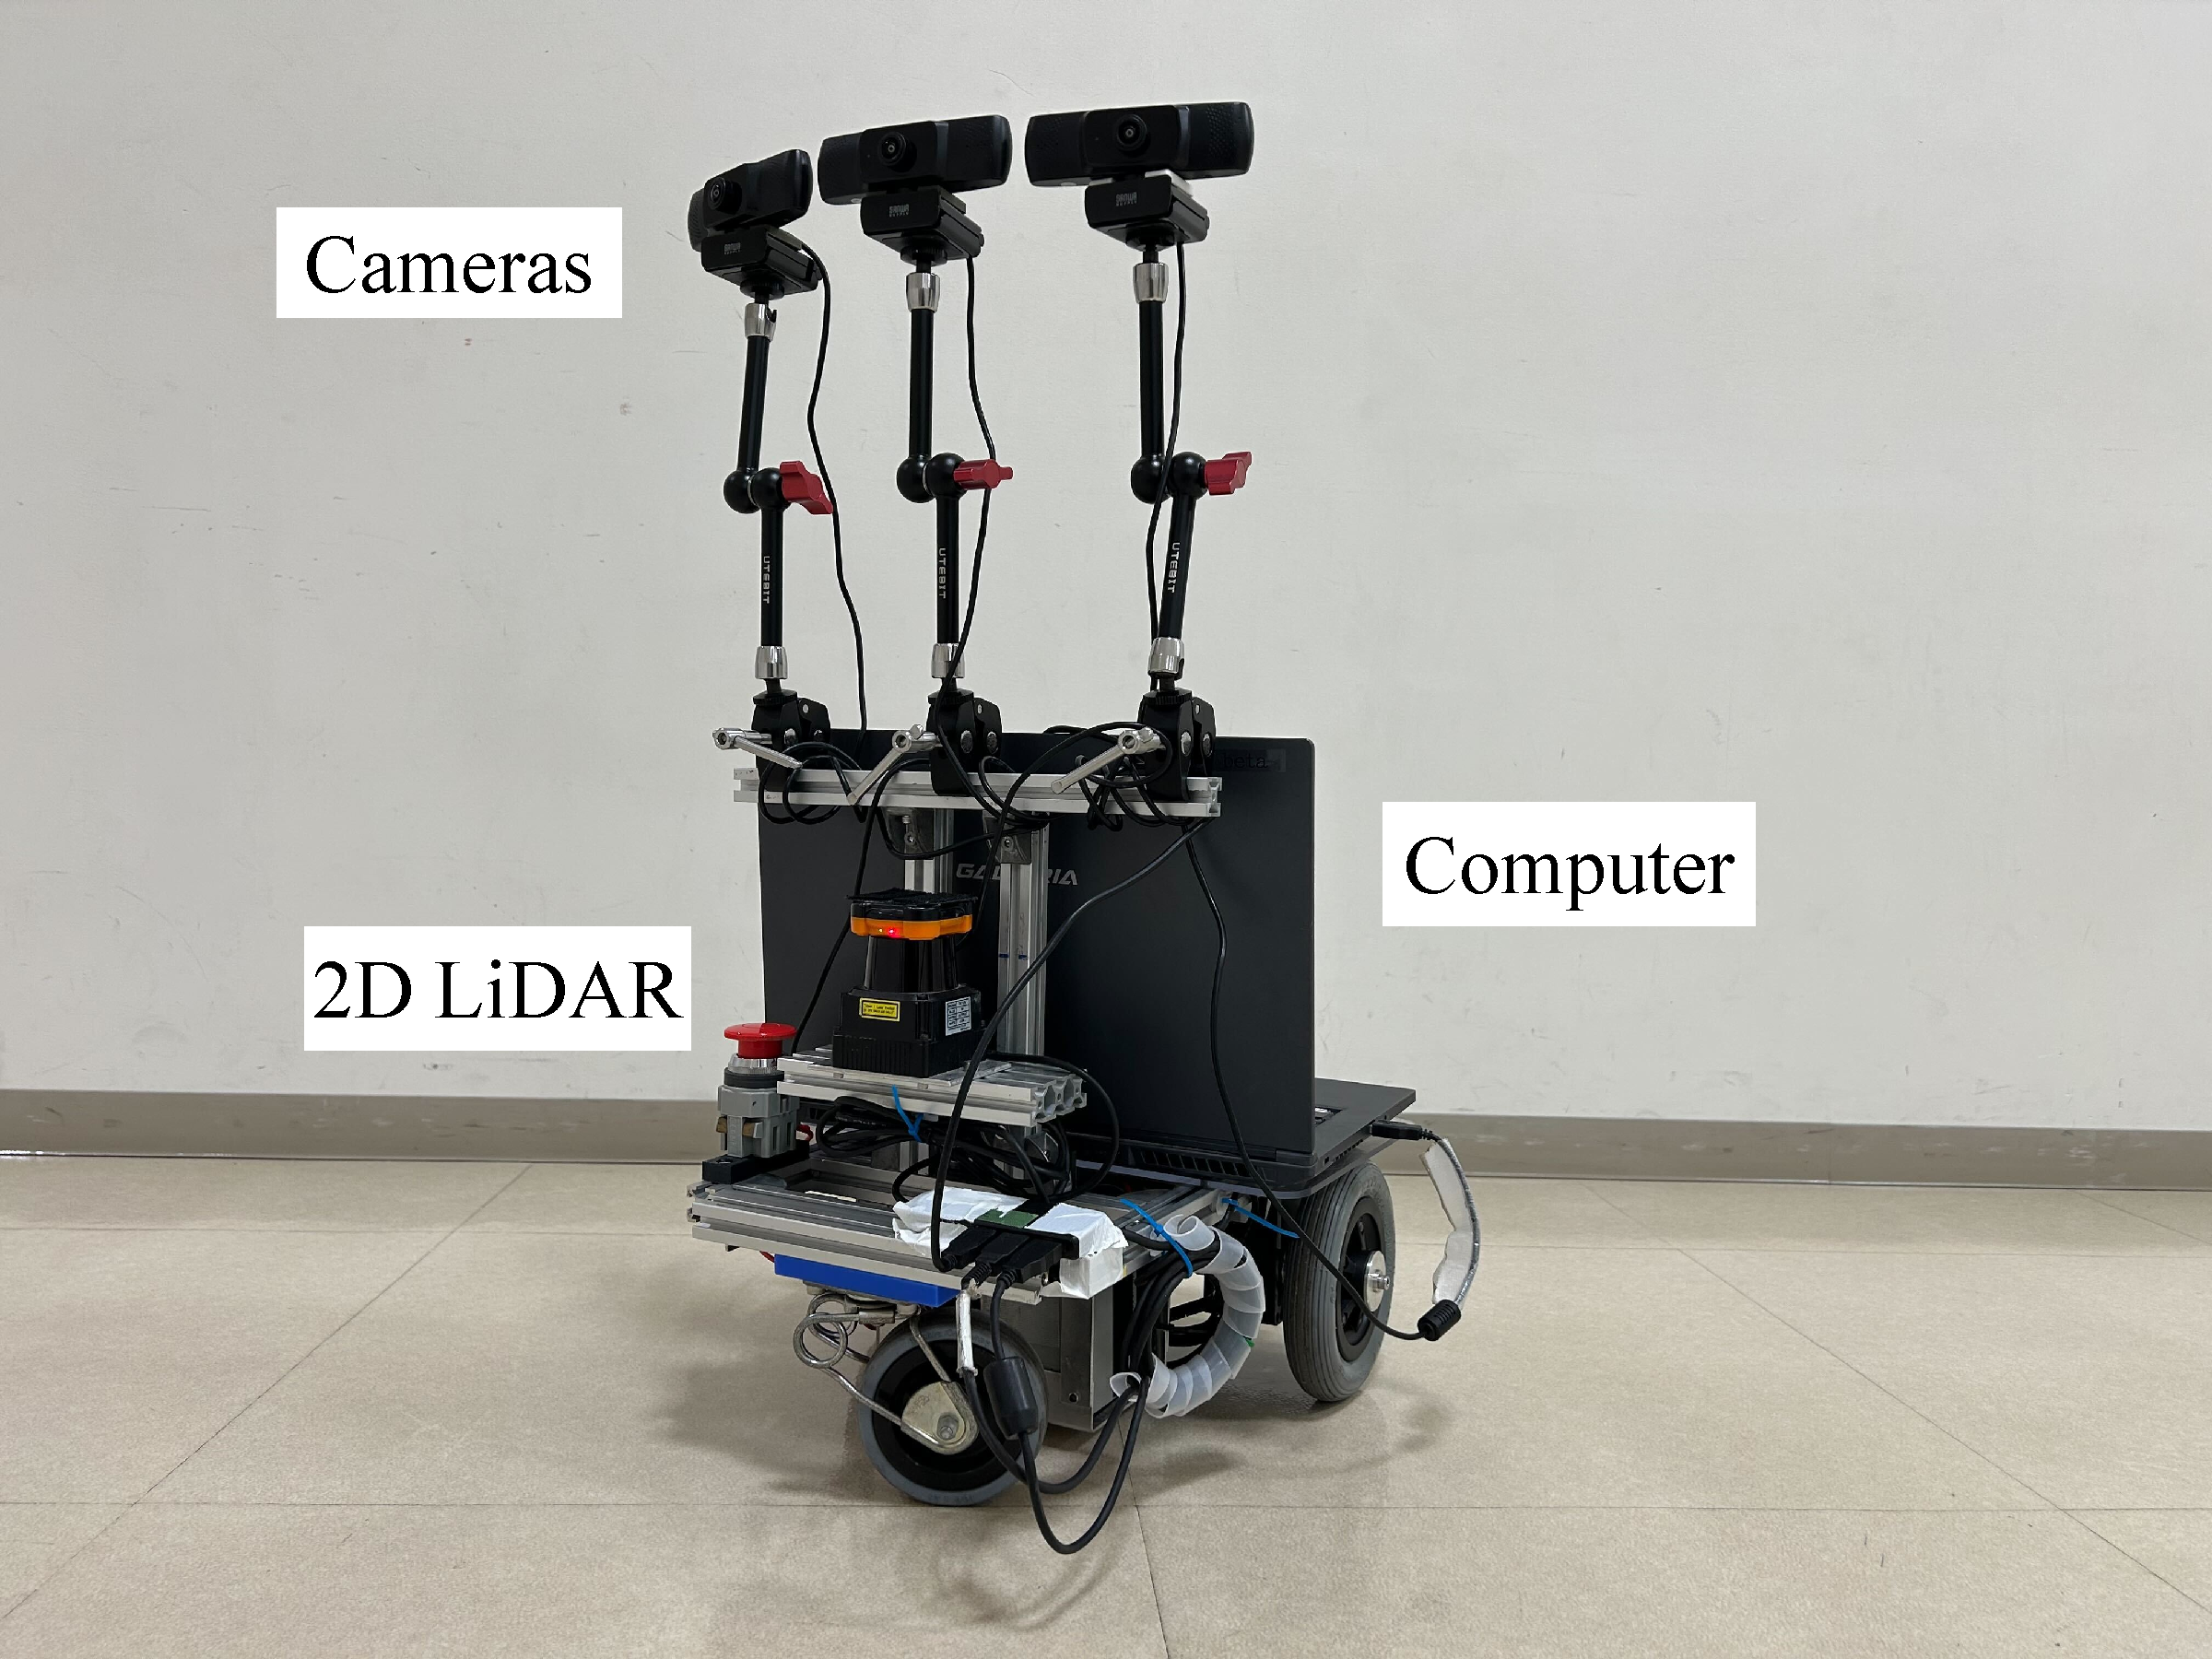
\includegraphics[width=60mm]{images/pdf/ishiguro/gamma.pdf}
     \caption{Experimental setup}
     \label{fig:gamma}
\end{figure}
\newpage
\section{実験方法}
\subsection{実験環境}
実験環境として\figref{fig:topo}に示す千葉工業大学 2 号館 3 階を用いる.
環境中には,三叉路が 6 つ,角が 3 つ,突き当りが 4 つ含まれている.
また,経路追従モジュールと通路分類モジュールの学習データを収集するために,\figref{fig:route}に示すルートを走行する.

\begin{figure}[htbp]
  \centering
  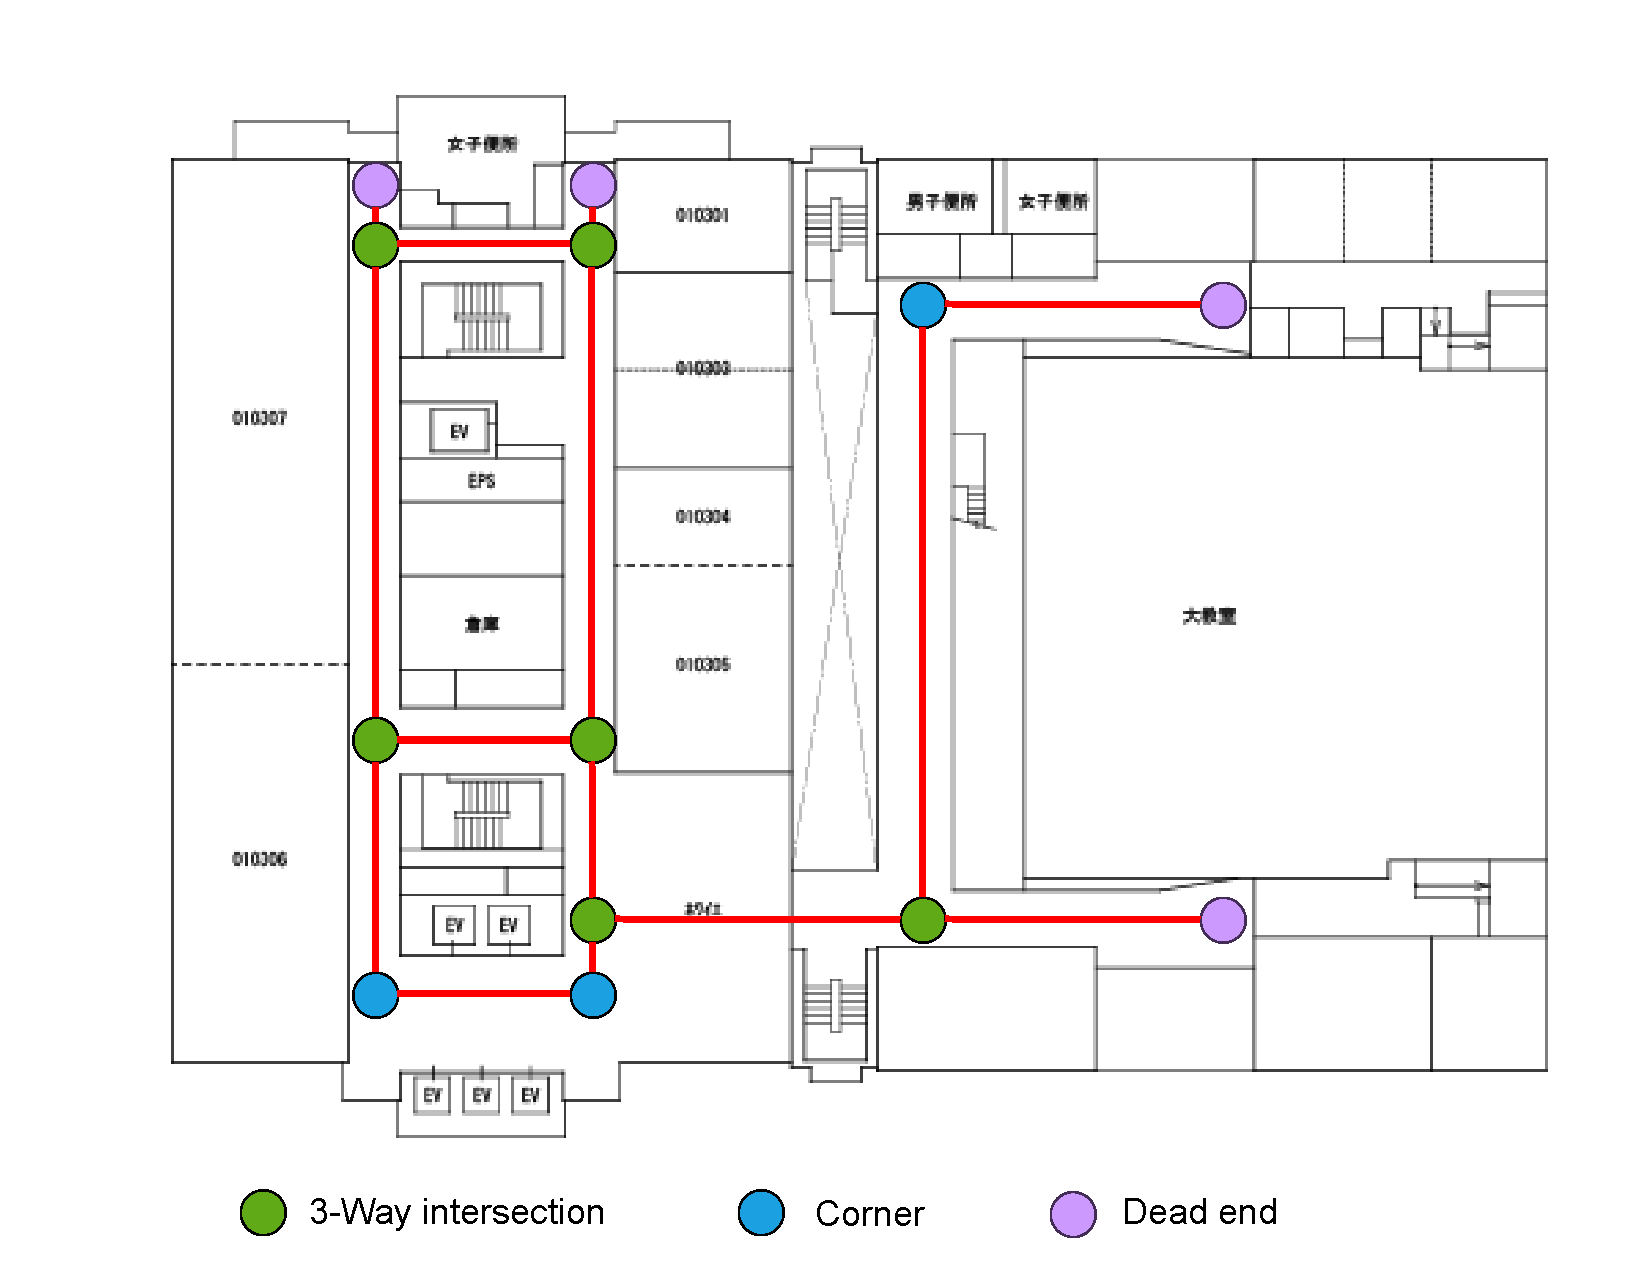
\includegraphics[width=130mm]{images/pdf/ishiguro/topo.pdf}
  \caption{Experimental environment}
  \label{fig:topo}
\end{figure}

\begin{figure}[h]
  \centering
  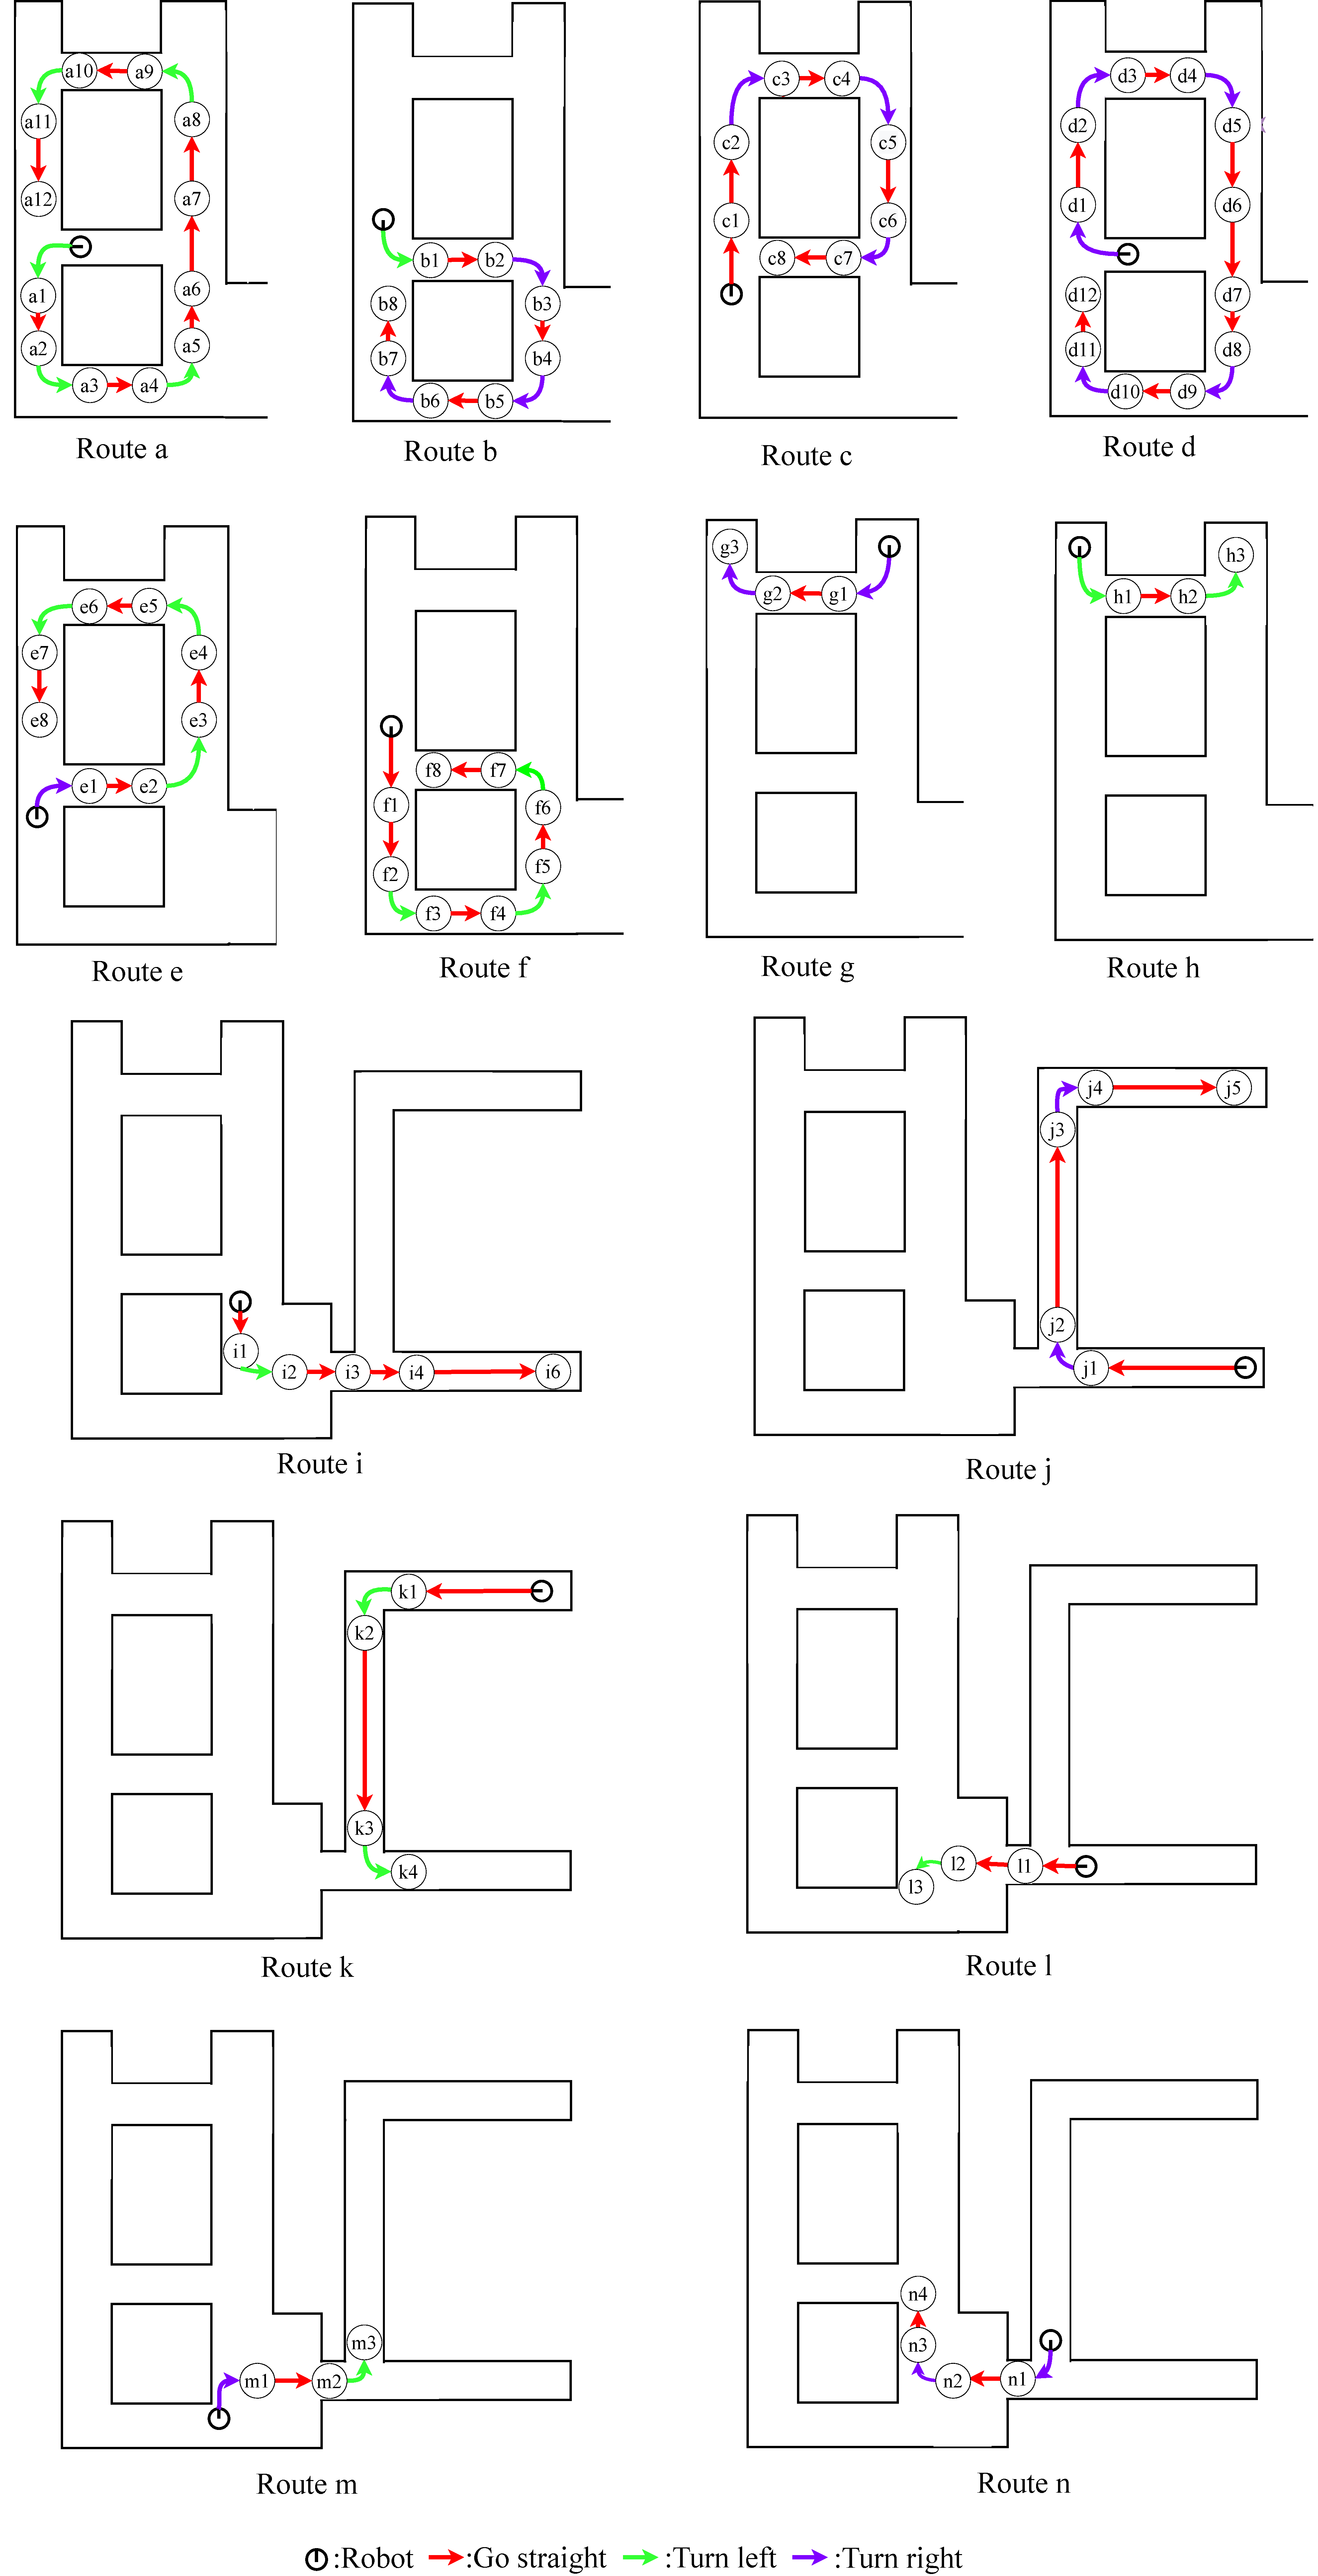
\includegraphics[width=100mm]{images/pdf/ishiguro/route.pdf}
  \caption{Route used for learning}
  \label{fig:route}
\end{figure}

\newpage
\subsection{シナリオの選定}
実験に使用するシナリオを,島田らが作成した 50 例から選定した.
選定するにあたって,以下の条件を設定した.

\begin{enumerate}
  \item [1)] ロボットが移動するには通路が狭すぎて,衝突せずに走行するのが困難な,\figref{fig:keepout}上部に示す部分を走行ルートに含まれないこと.
  \item [2)] 現時点の経路追従モジュールでは対応していない,「後ろを向く」などその場での旋回が含まれていないこと.
  % \item [3)] ロボットが移動しても,カメラ画像の特徴の変化が小さいため,通路の種類の分類が困難な\figref{fig:keepout}下部に示す部分がスタート地点では無いこと.
  \item [3)] スタート地点が\figref{fig:keepout}に示す箇所でないこと.この箇所がスタート地点のシナリオは,「左手に通路が見えるまで直進」か「右手に通路が見えるまで直進」である.現時点の路分類モジュールの入力である正面のカメラ画像からでは,ロボットが移動してもカメラ画像の特徴の変化が小さく,シナリオの条件を満たす通路分類結果が得られない可能性がある.
\end{enumerate}

条件ごとの除外したシナリオ数を\tabref{tab:remove}に示す.
また,条件 2 と 3 の両方を満たしたシナリオが 2 つある. 
これにより,選定されたシナリオ数は 28 例となる.
\begin{table}[htbp]
  \centering
  \caption{Number of scenarios excluded}\label{tab:remove}
  \begin{tabular}{c|c}
  \hline
  reason & number of secnario\\
  \hline
  1  & 4\\
  2  & 7\\
  3  & 13\\
  \hline
  \end{tabular}
\end{table}

\begin{figure}
  \centering
  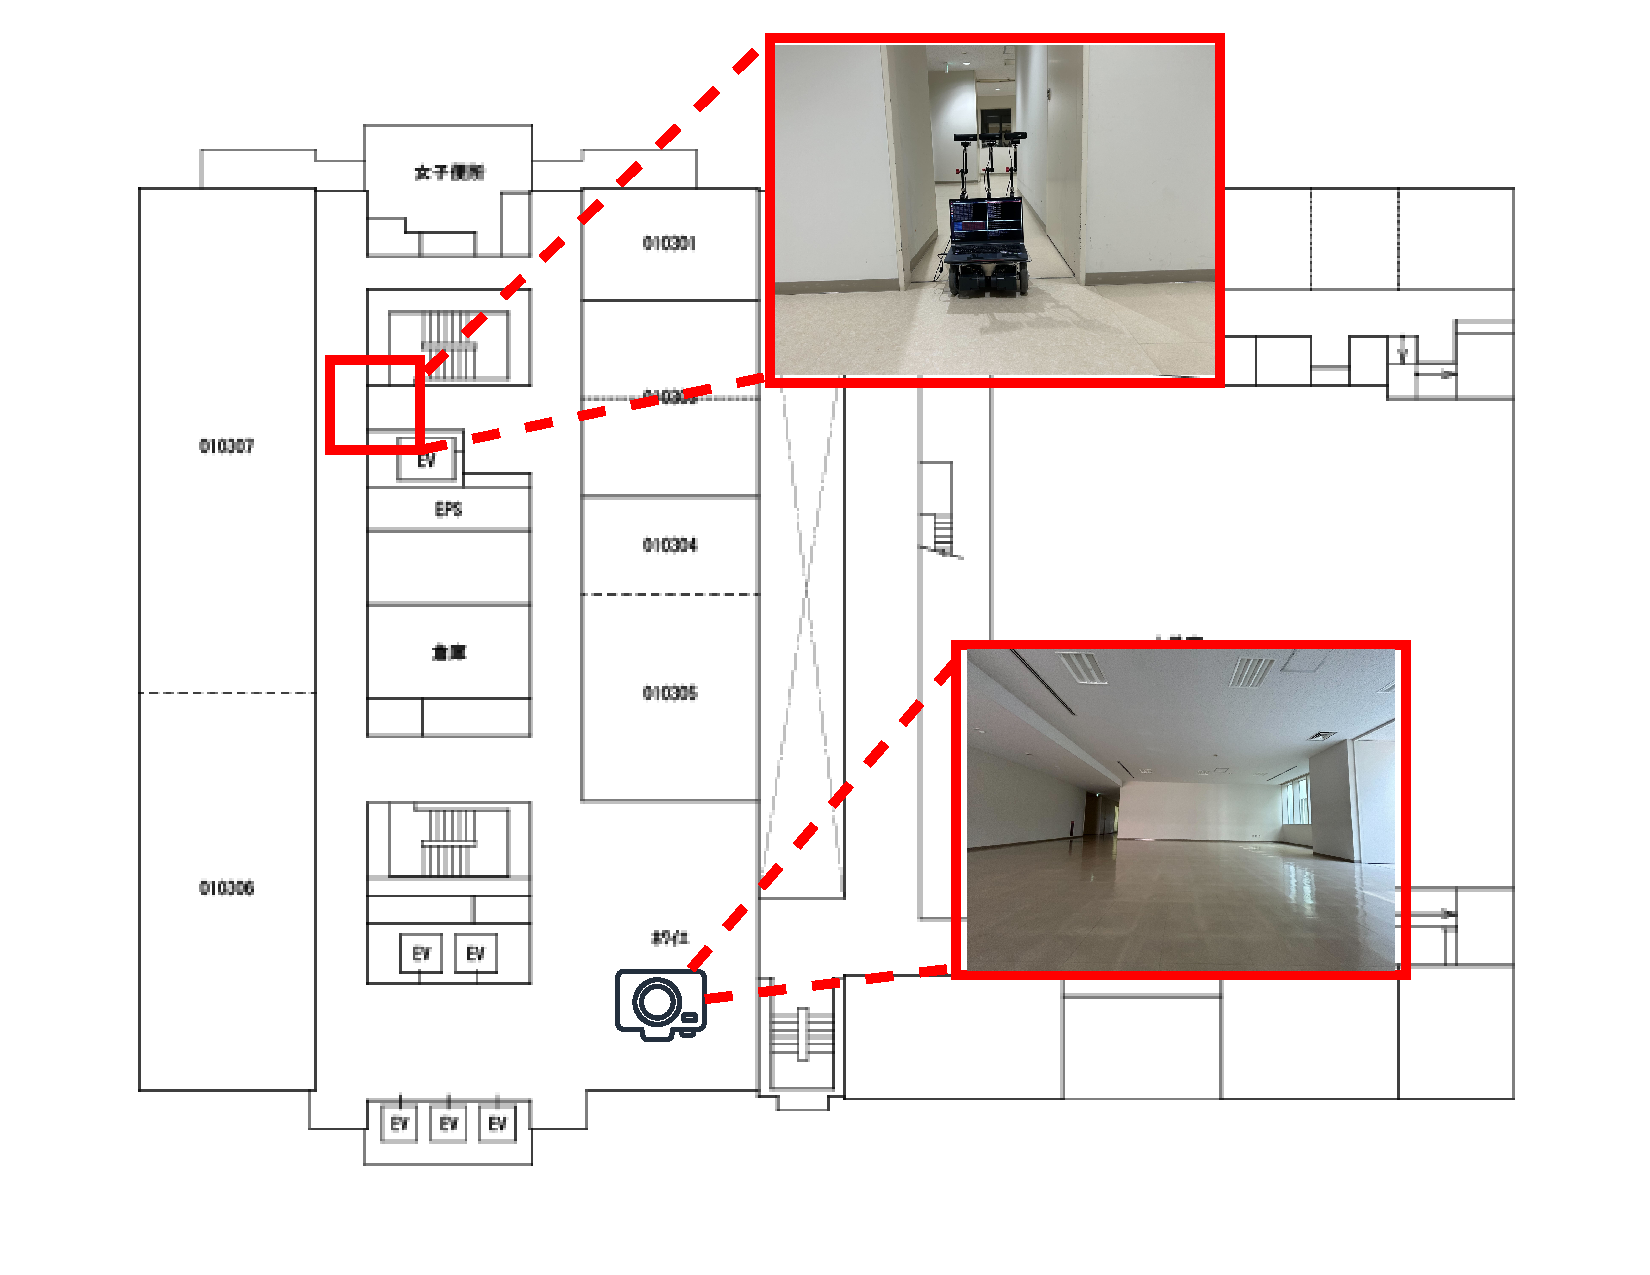
\includegraphics[width=130mm]{images/pdf/ishiguro/keepout.pdf}
  \caption{Excluded area for experiments}
  \label{fig:keepout}
\end{figure}

\clearpage
\subsection{経路追従モジュールの訓練}
\figref{fig:route}に示すルートをオンライン学習させながら 1 周走行する.
データセットの収集には藤原ら\cite{fujiwara2023}が提案する手法を用いる.
また,オンライン学習で作成したモデルに追加でオフライン学習を行う.
オフライン学習時のデータセットにはオンライン学習の際に作成したルート 1 周分のデータを用いる.
データセットからはオンライン学習と同様のバッチサイズ 8 でデータをランダムに取得し,epoch数は 20 とした.

\subsection{通路分類モジュールの訓練}
\figref{fig:route}に示すルートをROS の navigation パッケージを使用して,経路を 1 周する.
その際, 3 つのカメラからそれぞれ画像データを収集しながら走行する.
学習時のパラメータとして,バッチサイズを 32 ,epoch数を 30 とし,コストアプローチに用いた重みは\tabref{tab:cost}に示す.

\begin{table}[htbp]
  \centering
  \caption{The weights assigned to each class in the experiment}\label{tab:cost}
  \begin{tabular}{c|c}
  \hline
  Class & Class weights\\
  \hline
  直進   & 1\\
  突き当たり   & 39.5\\
  角(右) & 14\\
  角(左)& 14.2 \\
  十字路 & 1  \\
  三叉路(右)& 6.6  \\
  三叉路(中央)& 7.0  \\
  三叉路(左) & 6.4  \\
  \hline
  \end{tabular}
\end{table}

\clearpage
\subsection{シナリオに基づくナビゲーション}
2 つのモジュールを訓練後,ロボットが目的地まで到達できるか確認する.
実験では,ロボットをシナリオのスタート地点,向きに配置し,シナリオを 1 例ずつ入力する.
壁に衝突することなく正しい経路を選択し,目的地で停止した場合に成功とする.
%
%% Main Matter
\mainmatter{}
%
\chapter{序論}
\label{chap:introduction}
%
%\input{introduction/preface}
%
%!TEX root = ../thesis.tex

\section{背景}
移動ロボットにおけるナビゲーションは,目的地までロボットを誘導する制御技術として広く利用されており,物流や,農業,製造業などで活用されている.
一般的には, LiDAR や IMU ,ホイールエンコーダなど複数のセンサから得られるデータと占有格子地図などのメトリックマップを使用することでロボットを目的地まで制御する.
一方で,後述するようにカメラ画像と深層学習に基づくナビゲーション技術の研究も進んでいる.

Felipe ら\cite{codevilla2018endtoend}は視覚を入力とした end-to-end 学習により自動運転を行う手法において,右折や左折といった行動をネットワークの入力に加えることで,性能が向上することを報告している.
本研究室の岡田ら\cite{okada2020}\cite{okada2021}は,\figref{fig:imitation_sys}にように,メトリックマップに基づく経路追従行動を視覚を入力として模倣学習することで,視覚に基づて経路追従するシステムを提案した.
この手法では,センサとメトリックマップを入力としたルールベース制御器によって生成されたヨー方向の角速度とロボットに取り付けたカメラから取得した RGB 画像をペアにしてデータセットに加えて学習する.
学習後はカメラ画像のみを用いて,学習した経路を追従できることが確認されている.
% この手法では,センサとメトリックマップを入力とした ROS の navigation パッケージによって生成されたナビゲーションの角速度とカメラ画像をペアにして学習し,学習後はカメラ画像のみを用いて経路追従行動できることが確認されている.
% この手法では,一般的な模倣学習が人間のステアリング操作を模倣するのに対し,ナビゲーションシステム自体の行動を模倣する点で特徴的であり,データセットの収集を自動で行うことができる.
% これらの技術の有効性は,シミュレーションおよび実ロボットの実験により検証されており,視覚に基づくナビゲーションで一定の経路追従性能を達成できることが確認されている.
\begin{figure}[h]
     \centering
     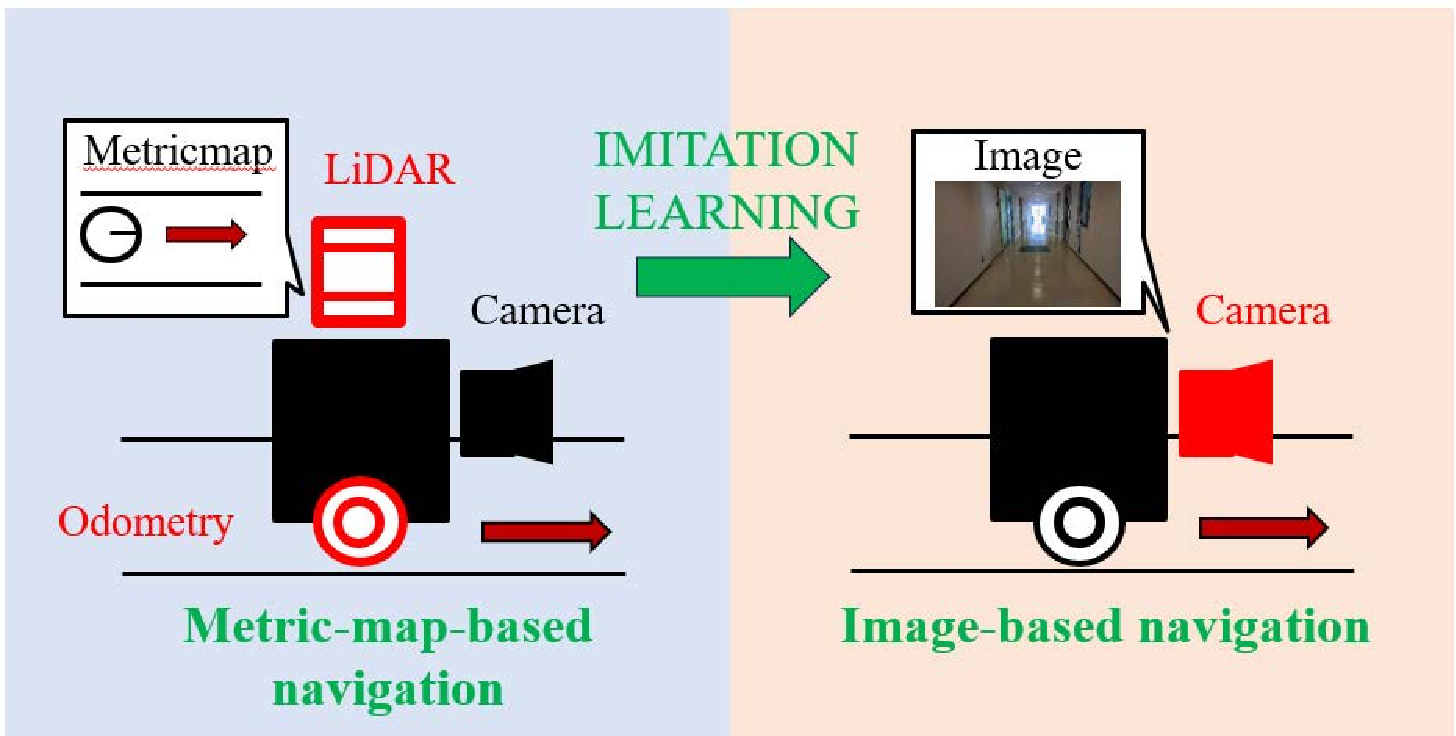
\includegraphics[width=120mm]{images/pdf/ishiguro/system.pdf}
     \caption{Imitation method of path-tracking behavior}
     \label{fig:imitation_sys}
\end{figure}

また,春山ら\cite{haruyama2023}はカメラ画像とシナリオに基づいて,任意の目的地まで経路追従するシステムを提案している.
ここでのシナリオとは島田ら\cite{shimada2020}が提案した,「条件」と「行動」に関する単語を組みわせて構成する文章を指す.
春山らの手法では,岡田らの視覚に基づいたナビゲーションに加え,カメラ画像から通路の種類を分類,シナリオによって目標方向を決定し,経路を選択する機能を追加している.
春山らの先行研究では,島田らが提案した 50 例のシナリオの中から対象としている 7 例すべてで経路追従が可能であることを確認している.

春山らの先行研究では,島田らが作成したシナリオの中で,以下\figref{fig:cit3f}の青枠で示すエリアを対象としたシナリオを用いている.
このエリアはホワイエと呼ばれるスペースを一部を含むものの,壁や床の色が類似しており,一貫性のある環境といえる.
一方で\figref{fig:cit3f}の赤色で示すエリアを含むシナリオでは,地面の色が異なるエリアやホワイエも対象としており,視覚に基づいて経路追従するのがより困難な環境と考えられる.
また,春山らの先行研究では対象としたシナリオすべてで目的地まで到達できることが確認されており,失敗の要因は判明していない.
失敗する場合は要因を調査することで,システムの改良点について考察できるようになる.

また,カメラ画像と深層学習に基づくナビゲーションの先行研究では,Felipeらが目標方向ごとにモデルを切り替えるネットワークが経路追従の成功率を高められると報告している.
提案されたネットワークを使用することで,春山らが使用していたネットワークより経路追従の成功率を向上させることができる可能性がある.

\begin{figure}[htbp]
     \centering
     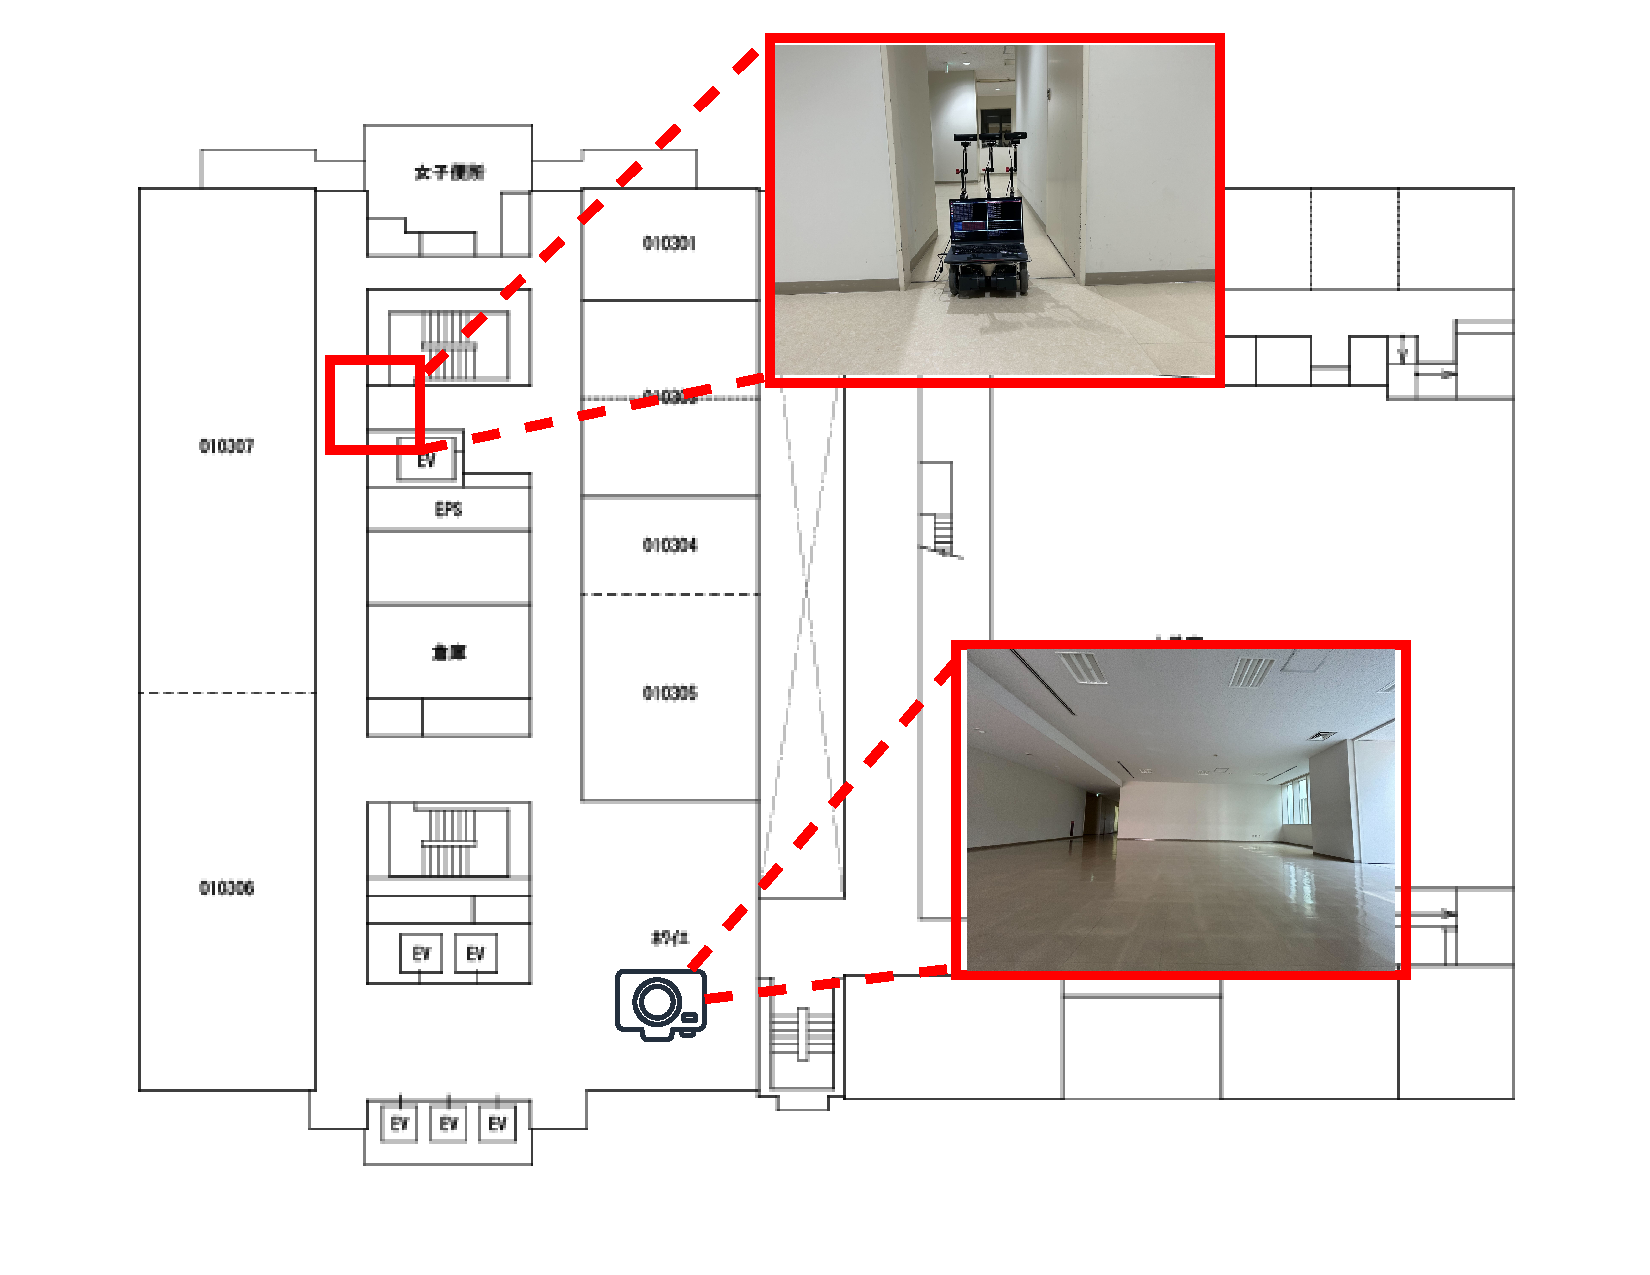
\includegraphics[width=130mm]{images/pdf/ishiguro/cit3f.pdf}
     \caption{Experimental environment}
     \label{fig:cit3f}
\end{figure}

\newpage

%
\section{目的}
本論文では,島田らが作成したシナリオにおいて春山らの実験では検証されていないシナリオでも,目的地までカメラ画像のみを入力として経路追従できるかを,実ロボットを用いた実験により確認する.
また,経路追従の成功率を高めるためにシステムに改良を加える.
%
\section{論文構成}
第1章では,先行研究や背景,本論文の目的について述べた.
第2章では,本研究に関連する技術について述べる.
第3章では,関連研究について述べる.
第4章では,先行研究からの変更点について述べ,シミュレータを用いた実験によって有効性を調査する.
第5章では,実ロボットを用いた実験について述べる.
第6章では,本論文について結論を述べる.

%ここにディレクトリのパスを追加していく
\chapter{要素技術}
\section{メトリックマップに基づくナビゲーション}
メトリックマップに基づくナビゲーションについて説明する.
ナビゲーションを実現するためには,LiDARやオドメトリなどのセンサとメトリックマップを活用し,自己位置推定や経路計画を行うことで,ロボットが目的地まで自律的に移動する仕組みが必要となる.
はじめに自己位置推定を行い,ロボットが地図上のどこに位置しているかを特定する.
これには,LiDARやオドメトリデータなどのセンサ情報を利用したアルゴリズムである,AMCL(Adaptive Monte Carlo Localization)などを活用する.
次に,推定した自己位置から目的地までの最適な経路を計画する.
計画された経路に基づき,ロボットの動作をリアルタイムで制御を行う.
メトリックマップに基づくナビゲーションの利点として,事前に取得した環境情報を有効活用できる点が挙げられる.
一方で,事前に取得した環境情報と現在の環境情報が大きく異なる場合,自律移動が失敗する可能性高まることが課題となる.
\figref{fig:nav}にメトリックマップに基づくナビゲーションの例を示す.
本論文ではメトリックマップに基づくナビゲーションを教師として模倣学習を行う.

\begin{figure}[htbp]
  \centering
  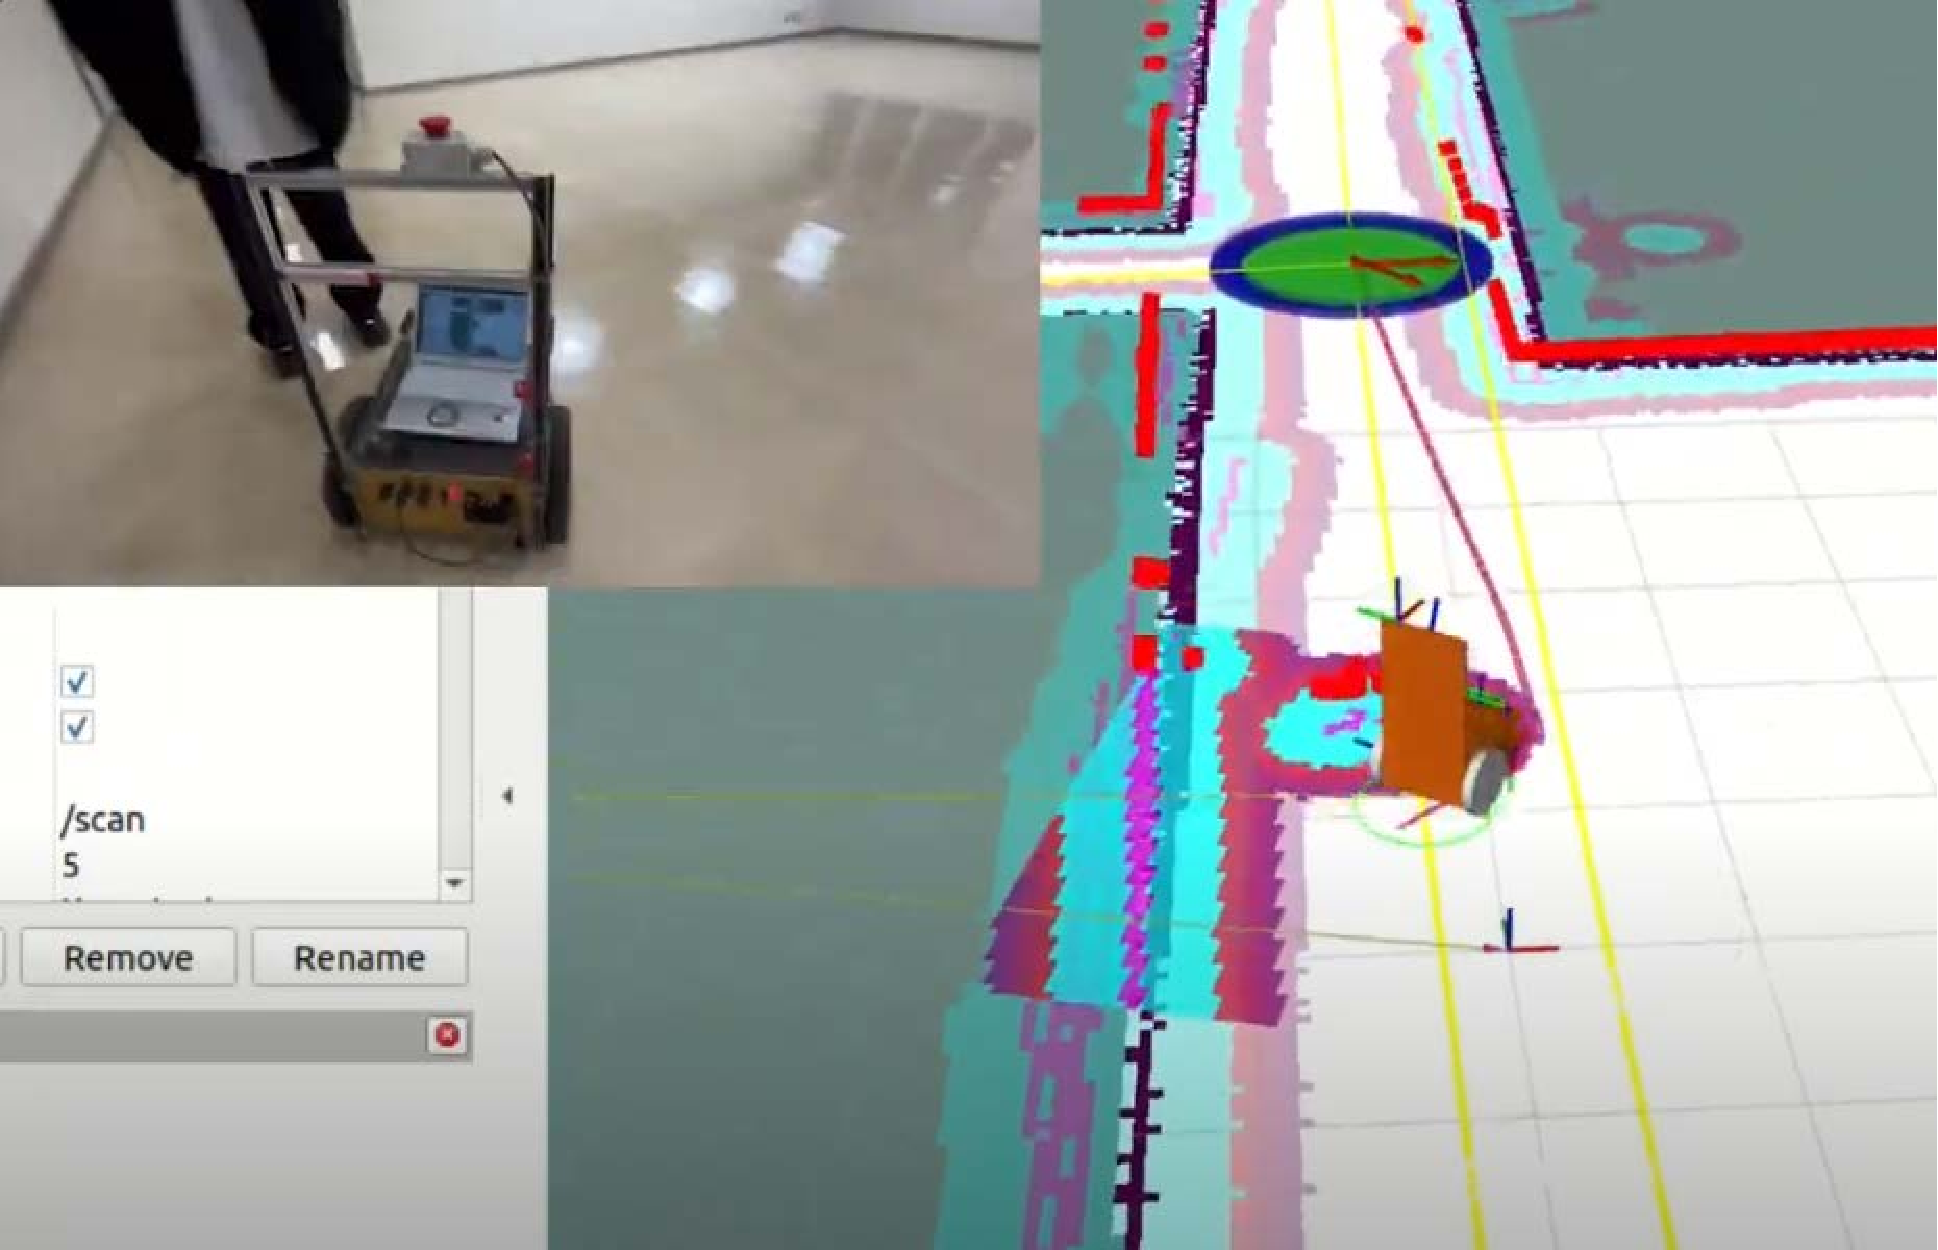
\includegraphics[width=130mm]{images/pdf/other/nav.pdf}
  \caption{Navigation based on metric map}
  \label{fig:nav}
\end{figure}
\chapter{先行研究}
\label{chap:prior}
本論文の議論のベースとなる,岡田らの従来手法と島田らが提案したトポロジカルマップの形式,単語の組み合わせによる経路の表現であるシナリオについて述べたのち,春山らの視覚に基づいて目的地まで自律移動するシステムについて述べる.
\section{視覚と行動の end-to-end 学習により経路追従行動をオンラ
インで模倣する手法}
岡田らの手法では,メトリックマップに基づく経路追従行動を視覚を入力とした行動へ模倣するために,end-to-end学習を用いた手法を提案している.
ロボットは経路を自律移動するのと同時に学習を行う.
手法に基づいて構築されたシステムを\figref{fig:okada_sys}に示す.

\begin{figure}[htbp]
  \centering
   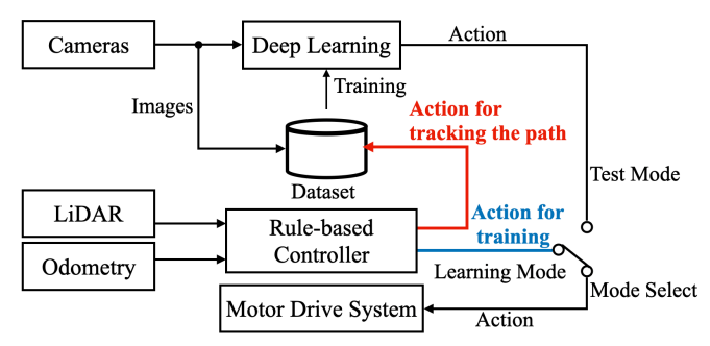
\includegraphics[width=100mm]{images/pdf/okada/method_sys.pdf}
   \caption[Structure of the Okada and others proposed system]{Structure of the Okada and others proposed system(Quoted from\cite{okada2020})}
   \label{fig:okada_sys}
\end{figure}

訓練時には,ROS の navigation パッケージ \cite{ros}を使用して,設定した経路を追従する.
ロボットの並進速度は 0.2 m/sに固定する.
その際,ロボットに取り付けたカメラから取得した RGB 画像とルールベース制御器が出力するヨー方向の角速度をペアにして, 0.2 秒の周期でデータセットに追加する.
収集には 3 台のカメラを使用することで,データの多様性を高めるとともに過学習を防ぐ効果を狙っている.
また,左右のカメラ画像に対するヨー方向の角速度には経路復帰を補助するためのオフセット(\(\pm 0.2\)rad/s)を加える.

\newpage
\figref{fig:okada_net}に岡田らの従来手法における学習器のネットワーク構造を示す.
% 学習器は入力をRGB画像データ,出力をロボットのヨー方向の角速度としている.
ネットワークは,入力層 1,畳み込み層 3,全結合層 2,出力層 1 の全7層で構成される.
データセットからはバッチサイズ 8 で教師データを抽出し, end-to-end 学習を行う.

\begin{figure}[htbp]
    \centering
     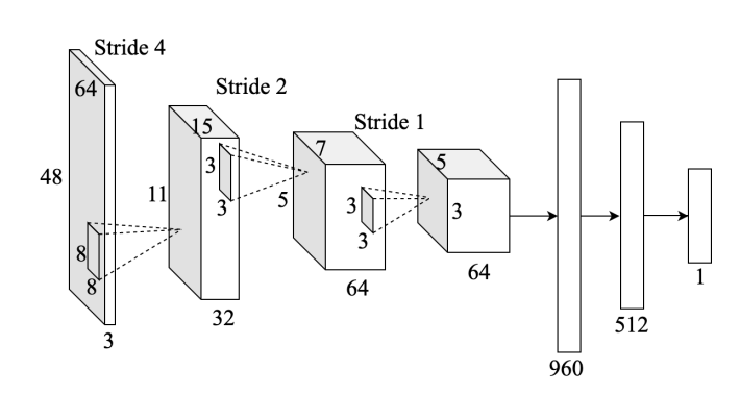
\includegraphics[width=100mm]{images/pdf/okada/network.pdf}
     \caption[Structure of the network Okada and others used]{Structure of the network Okada and others used (Quoted from \cite{okada2020})}
     \label{fig:okada_net}
\end{figure}

学習器の訓練後は,中央のカメラから得た RGB 画像を入力とし,出力されるヨー方向の角速度を用いて経路を追従する.
% この手法は実ロボットを用いて有効性が調査されており,\figref{fig:cource}に示す学習した経路を,画像のみを入力とした学習器の出力で自律移動できることが確認されている.
この手法は実ロボットを用いて有効性が調査されており,学習した経路を画像のみを入力とした学習器の出力で自律移動できることが確認されている.
% \begin{figure}[htbp]
%   \centering
%    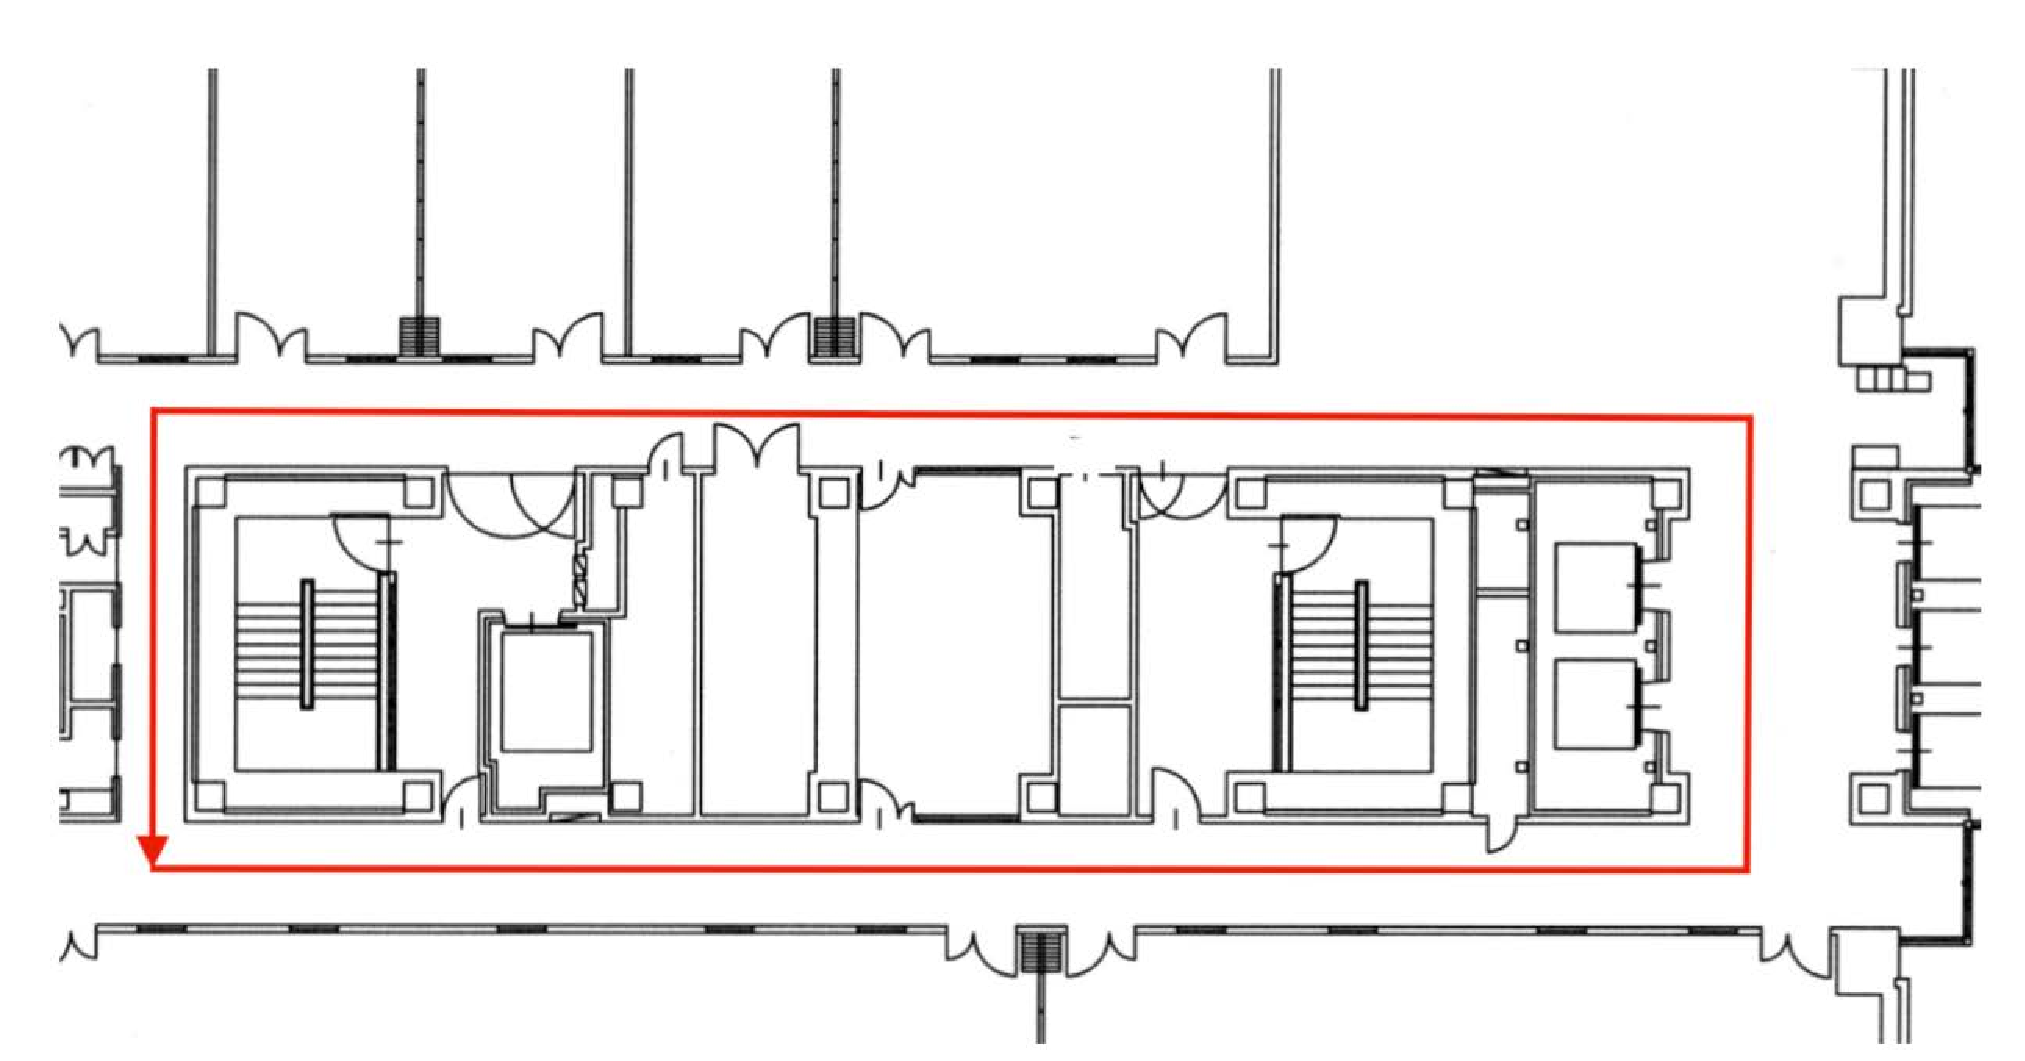
\includegraphics[width=80mm]{images/pdf/okada/cource.pdf}
%    \caption{Target path used in the experiment(Quoted from \cite{okada2020})}
%    \label{fig:cource}
% \end{figure}

\clearpage
\section{トポロジカルマップとシナリオ}
\subsubsection{トポロジカルマップ}
トポロジカルマップとは,環境をランドマークや特徴的な箇所をノードとし,その繋がりをエッジで表現した地図である.
島田らが提案したトポロジカルマップでは,ノードは通路の特徴的な箇所に配置され,エッジはノード間を接続する.
ノードにはID,通路の特徴(Type),エッジIDと相対角度(Edge)のデータが含まれ,エッジにはIDのみが含まれる.
この形式は道案内に関するアンケート結果に基づいており,人が道案内で「通路の特徴」や「向いている方向」を重視することが明らかになったことから設計された.

\begin{figure}[htbp]
  \centering
   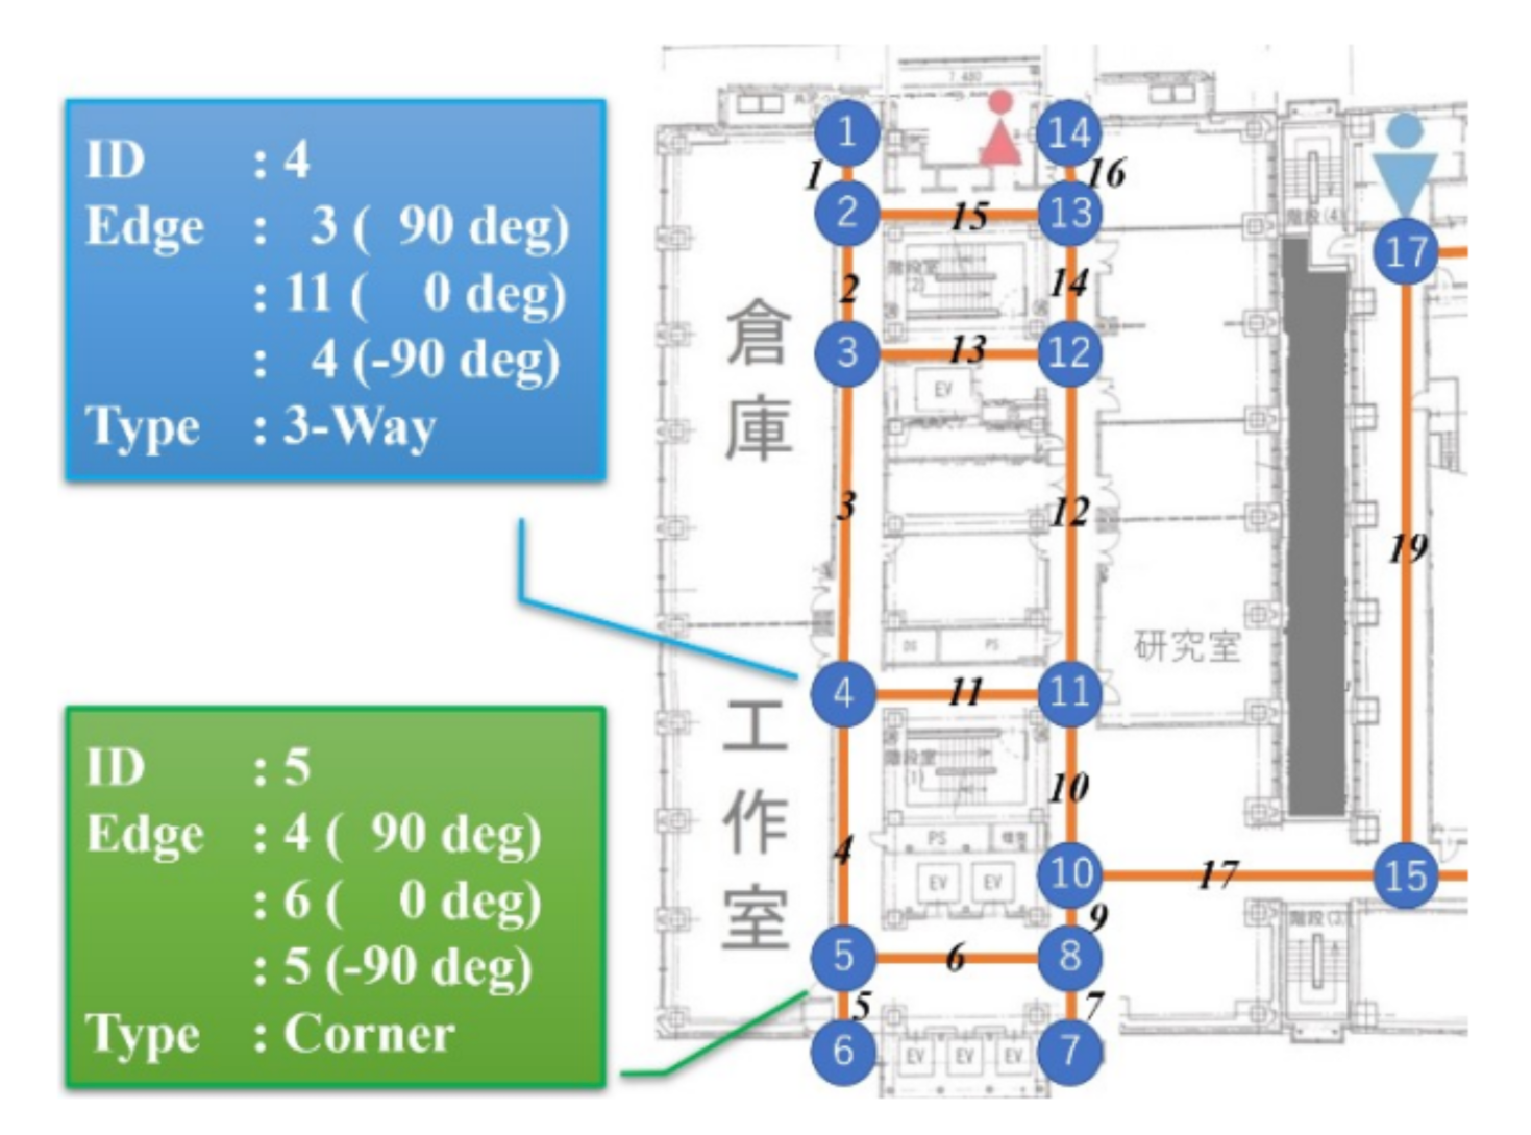
\includegraphics[width=80mm]{images/pdf/shimada/topo.pdf}
   \caption[Topological map format proposed by Shimada and others]{Topological map format proposed by Shimada and others(Quoted from\cite{shimada2020})}
   \label{fig:topo}
\end{figure}

\clearpage
\subsubsection{シナリオ}
シナリオは,トポロジカルマップ上の目的地までの経路を「条件」と「行動」の組み合わせで表現する手法である.
「条件」は「次の角」や「突き当たりまで」などを指し,「行動」は「直進」や「右折」などを指す.
この形式はトポロジカルマップ同様に道案内に関するアンケート結果に基づいており,人が「条件」と「行動」を組み合わせて道案内をすることが明らかになったことから設計された.
例として,特定の経路はと表現される.

\begin{figure}[htbp]
  \centering
   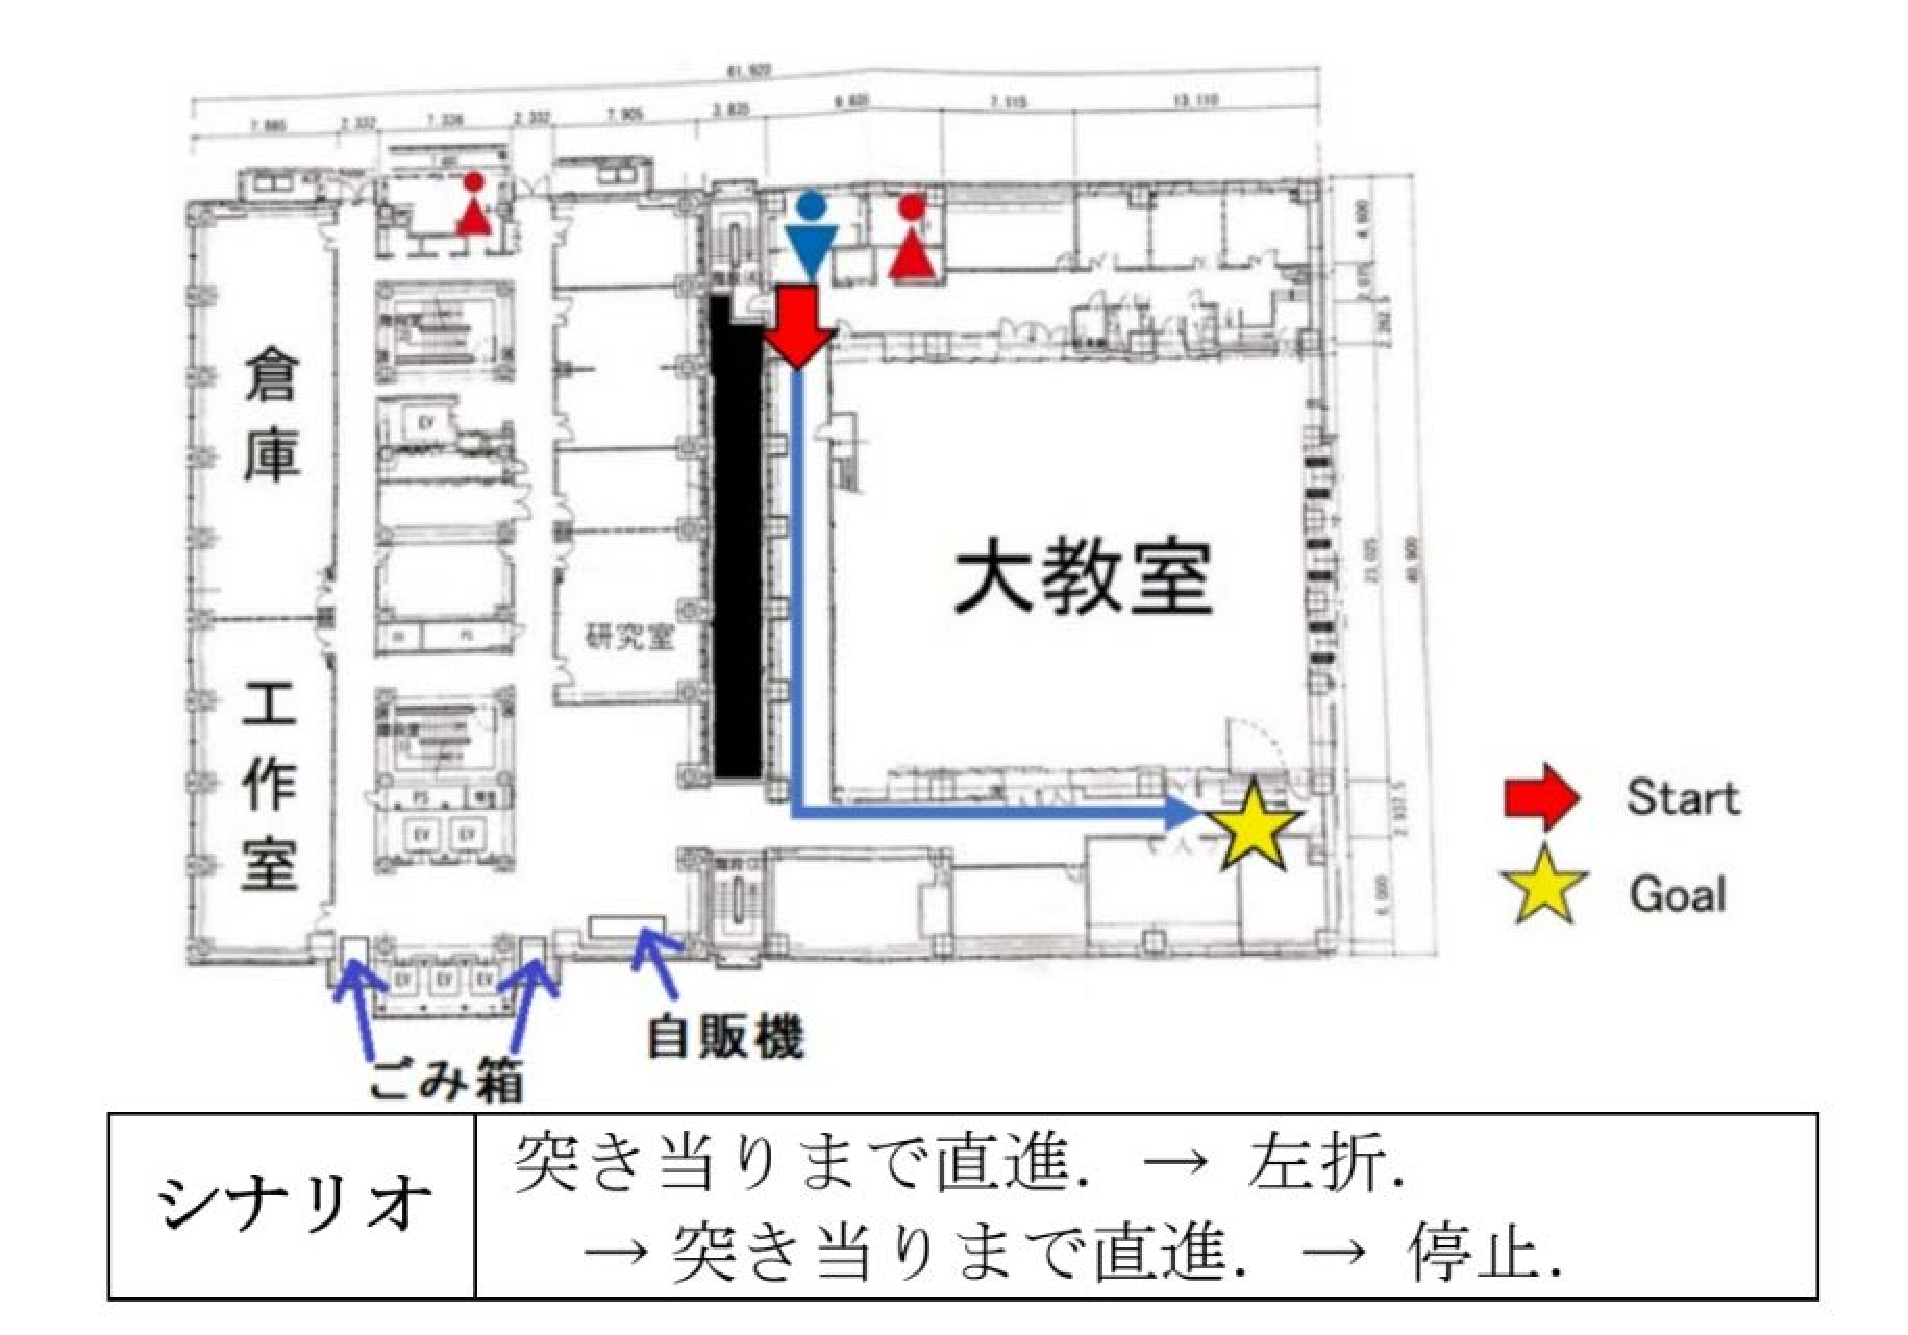
\includegraphics[width=90mm]{images/pdf/shimada/scenario.pdf}
   \caption{Topological map format proposed by Shimada and others(Quoted from\cite{shimada2020})}
   \label{fig:topo}
\end{figure}
\clearpage
\section{視覚に基づいて目的地まで自律移動するシステム}
春山らは,カメラ画像とトポロジカルマップから作成されるシナリオに基づいて,目的地まで自律移動するシステムを構築している.
提案されたシステムは,

1)カメラ画像と目標方向を与えることで,経路を追従するモジュール(以後,経路追従モジュールと呼ぶ)

2)シナリオを分解し,「条件」と「行動」を抽出するモジュール(以後,シナリオモジュールと呼ぶ)

3)カメラ画像から通路の特徴を分類するモジュール(以後,通路分類モジュールと呼ぶ)

の3つのモジュールで構成されており,それぞれについて述べる.
\subsection{経路追従モジュール}
このモジュールは,岡田らの手法から目標方向のデータを加えることで,分岐路で経路を選択し,移動する機能を追加したものである.
ここで目標方向とは,目標とする進行方向(「直進」や「右折」)を表す.
学習時は,カメラ画像とルールベース制御器が出力するヨー方向の角速度,目標方向を 0.2 秒周期でデータセットに加える.
データセットから抽出するバッチサイズや,カメラ画像の解像度は岡田ら手法と同様である.
データセットの収集には藤原らが提案した,データセットに加えるデータの不均衡を改善する手法,学習時に積極的な蛇行する手法を採用する.
\subsection{シナリオモジュール}
\subsection{通路分類モジュール}
このモジュールでは,ニューラルネットワークを用いることで,カメラ画像を入力として,通路の特徴を分類する.
データセットの収集をするために,ロボットをルールベース制御器に基づいて走行させる.
その際に,フレーム数 16 ,画像サイズ 64 × 48の連続したカメラ画像と通路の分類ラベルを1組として,0.125 秒周期でデータセットに加える.
通路の分類ラベルのアノテーションはルールベース制御器から出力されるラベルによって自動的に行う.
データセット内の不均衡を改善するために,クラス間のデータ数によって重み付けを行うコストアプローチを導入している.

実ロボットを用いた実験により,ロボットを目的地まで到達可能か検証されている.
実験では島田ら用いた 50 例のシナリオの中から,7例が用いられており,そのすべてでロボットが目的地へ到達できることが確認されている.
\chapter{機能の改善}
\label{chap:method}
経路追従モジュールに関して,経路追従の可能性を向上させるために2点変更を加えた.
変更点,理由について以下に述べる.
また,シミュレータを用いた実験により,それらの効果を調査する.
\section{ネットワークの変更}
春山らの先行研究では,\figref{fig:haruyama_net}に示すネットワークを使用していた.
一方で Felipe らは,コマンドによってモデルを切り替える形式のネットワークがより経路追従の成功率を高められると報告している.
そのため,今回の研究では Felipe らによって提案されたネットワークを参考に\figref{fig:branched}に示す,ネットワークを構築した.
ネットワークの入力は春山らが作成したものと同様の 64×48 の RGB画像と\tabref{tab:cmd_dir}に示す,目標方向のワンホットベクトルで,出力はヨー方向の角速度である.
また,損失関数や活性化関数などのパラメータは春山らの手法と同様である.

\begin{figure}[htbp]
  \centering
  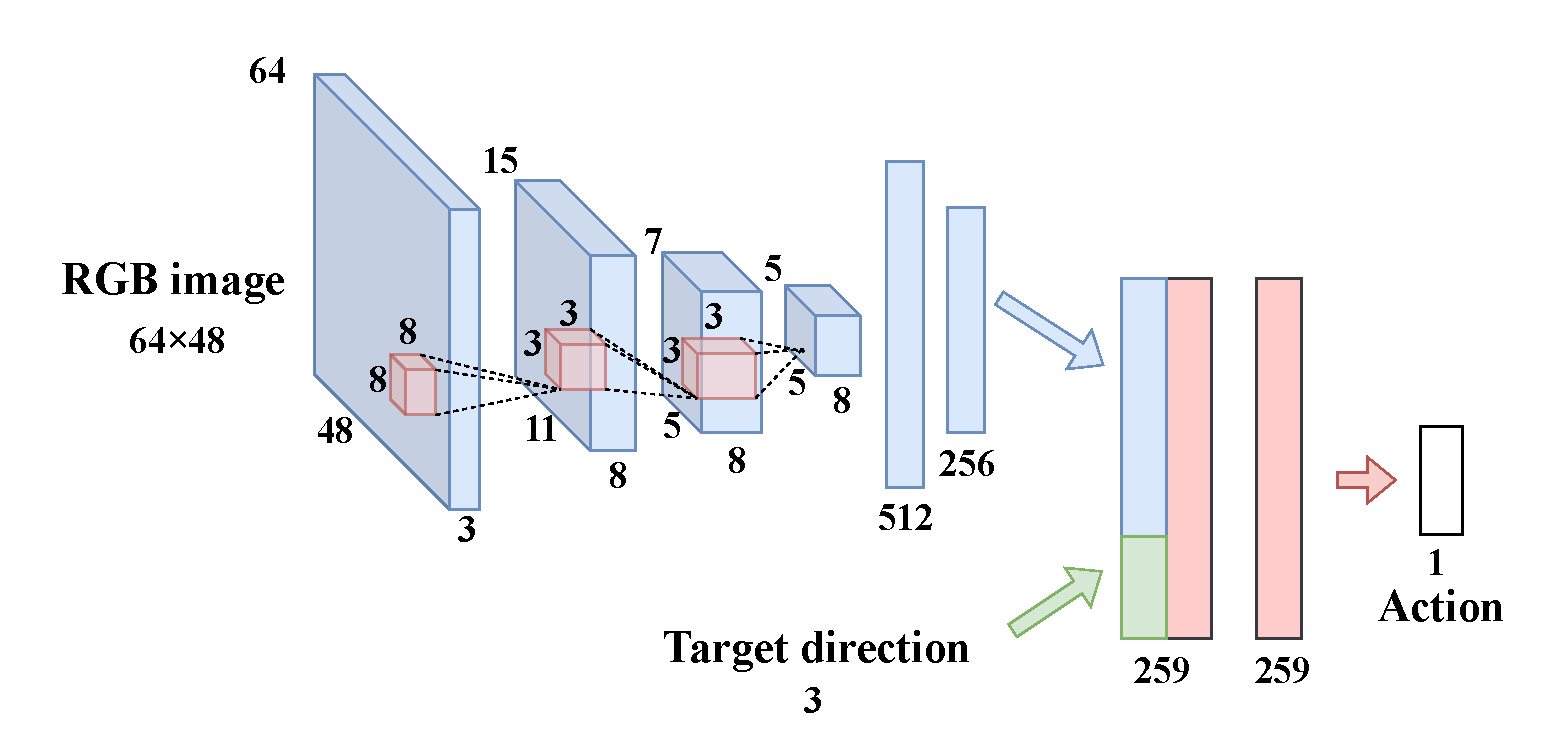
\includegraphics[width=110mm]{images/pdf/haruyama/net.pdf}
  \caption[Structure of the network haruyama and others used]{Structure of the network haruyama and others used(Quoted from \cite{fujiwara2023})}
  \label{fig:haruyama_net}
\end{figure}

\begin{figure}[htbp]
  \centering
   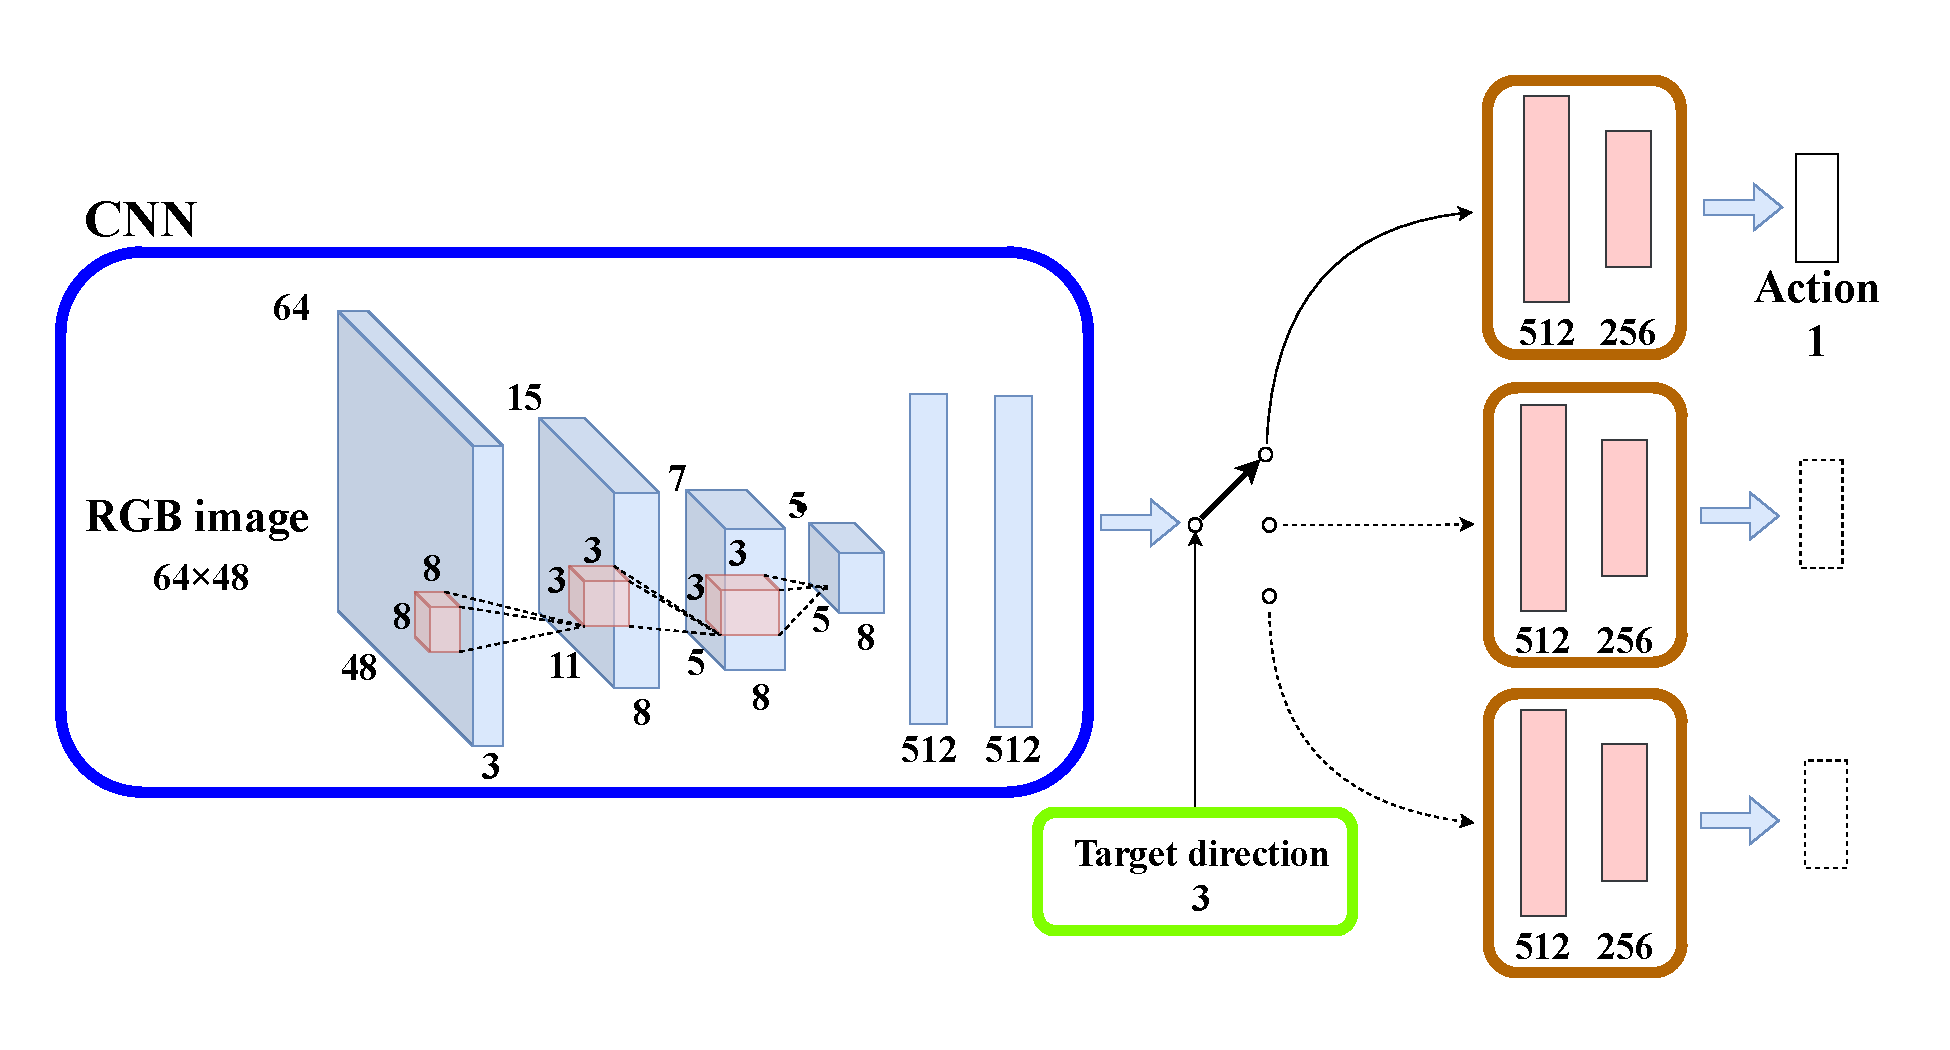
\includegraphics[width=110mm]{images/pdf/ishiguro/branched.pdf}
   \caption{Branched network}
   \label{fig:branched}
\end{figure}

\begin{table}[htbp]
  \centering
  \caption{Target direction and data for path-following module}\label{tab:cmd_dir}
  \begin{tabular}{|c|c|}
  \hline
  Target direction & Data        \\
  \hline
  Go straight   & {[}1,0,0{]} \\
  Turn left   & {[}0,1,0{]} \\
  Turn right   & {[}0,0,1{]} \\
  Stop   & {[}0,0,0{]}\\
  \hline
  \end{tabular}
\end{table}

\clearpage
\newpage
\section{オフライン学習}
春山らの先行研究では学習機の訓練に取得したデータを逐次学習するオンライン学習を用いていた.
オンライン学習の欠点として,学習するデータに偏りが発生してしまう点が挙げられる.
具体的には,学習の初期に取得したデータは学習される回数が多くなり,学習の後半に取得したデータは学習される回数が少ない.
これにより,学習が不十分な場合は経路追従できない箇所が生じることがある.
この欠点を補うために,オフライン学習を併用して行う.
% オンライン学習では学習データを収集しつつ,そのデータを学習に利用する一方で,オフライン学習は予め収集したデータを学習することですべてのデータを均等に学習できる.
オフライン学習とは一般的に用いられる学習方法で,予め収集したデータを使用して学習する手法を指す.
データを予め収集することにより,すべてのデータを同じ回数学習することが可能である.
本論文では,オンライン学習を最初に行い,そこで作成したデータセットを使用して学習することをオフライン学習と呼ぶ.

\section{シミュレータを用いた実験}
まずは,新たに作成したネットワークで経路を正しく選択できるかシミュレータを用いた実験により調査する.
次にオフライン学習を追加で行い,効果を検証する.

\subsubsection{実験装置}
シミュレータに Gazebo\cite{gazebo}を使用する.
ロボットには TurtleBot3 Waffle Pi\cite{turtlebot3}に3つのカメラを追加したモデルを用いる.

\subsubsection{実験環境}
実験環境として\figref{fig:haruyama_cit3f}に示す,千葉工業大学2号館3階を模した環境を使用する.
経路の選択を行う場所として\figref{fig:haruyama_cit3f}の A, Bの分岐路を対象に行う.
\figref{fig:select_pattern}に示すように,A,B の各分岐路で経路に侵入するパターンは 3 つ,また脱出するパターンがつ 2 つあることから合計 12 回の経路選択を行うことができる.

\begin{figure}
  \centering
  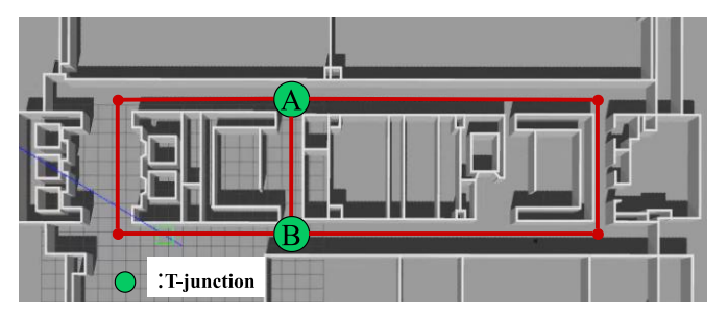
\includegraphics[width=130mm]{images/pdf/haruyama/cit3f.pdf}
  \caption[Experimental environment]{Experimental environment(Quoted from \cite{haruyama2022})}
  \label{fig:haruyama_cit3f}
\end{figure}

\begin{figure}
  \centering
  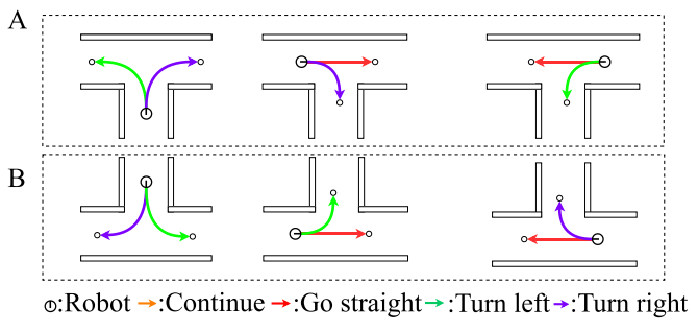
\includegraphics[width=130mm]{images/pdf/haruyama/select_pattern.pdf}
  \caption[Selecting a path the T-junction]{Selecting a path the T-junction(Quoted from \cite{haruyama2022})}
  \label{fig:select_pattern}
\end{figure}
 
\clearpage
\subsubsection{実験方法}
\figref{fig:fujiwara_route}に示す経路を, a から f の順番で走行しながら,模倣学習を行う.
データセットの収集には,藤原ら\cite{fujiwara2023}が提案している,学習データの不均衡を改善する手法,学習時の積極的な蛇行を行う手法を採用する.
テスト時は,学習器の出力で壁に衝突することなく,分岐路の先の経由点に到達することができれば成功とする.
オフライン学習に使用するデータセットは,a から f の順番で走行しながらオンライン学習を行った際に作成されるものを使用する.
オフライン学習のパラメータとして,バッチサイズはオンライン学習と同様の 8 でデータセットからランダムにデータを抽出し,epoch数は 10 とする.
実験では,学習とテストを繰り返し 10 回行う.

\begin{figure}
  \centering
  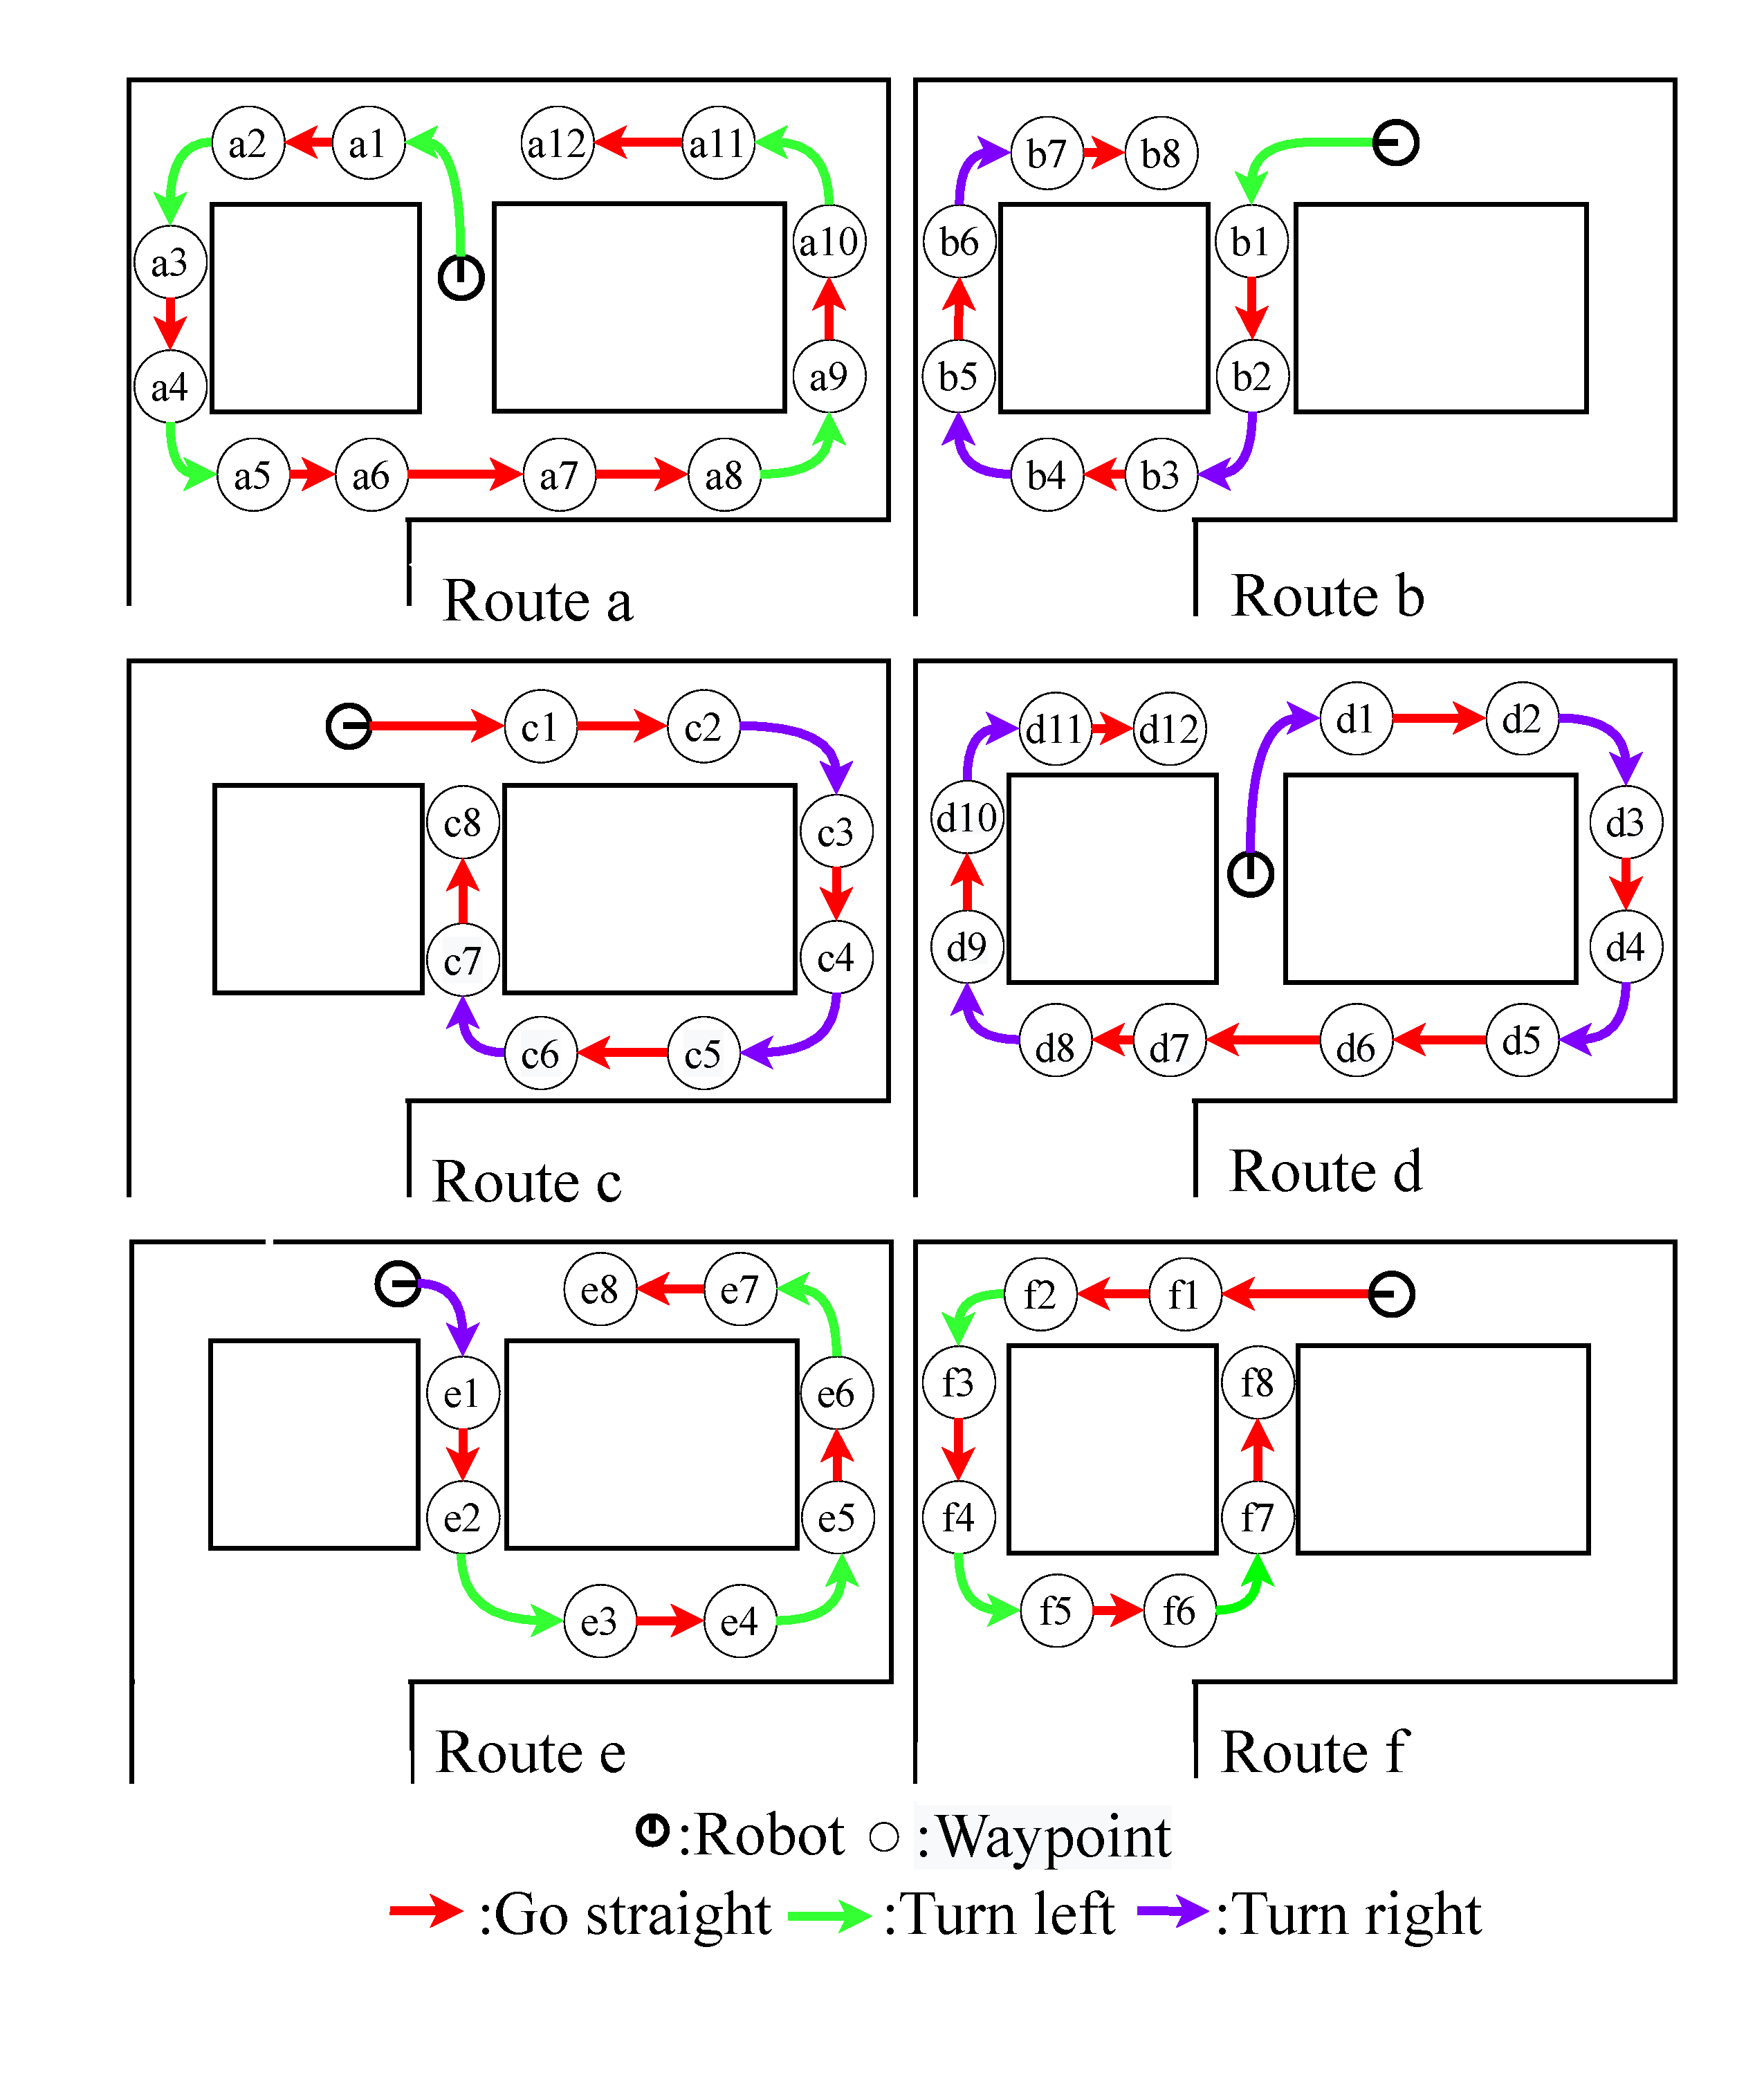
\includegraphics[width=130mm]{images/pdf/fujiwara/route.pdf}
  \caption[Route for experiment]{Route for experiment(Quoted from \cite{fujiwara2023})}
  \label{fig:fujiwara_route}
\end{figure}

\clearpage
\subsubsection{実験結果}
\tabref{tab:result}に結果を示す.
表では,春山らが使用していたネットワークを Previous network としている.
そして新たなネットワークを使用した実験を Branched とした.

新たに作成したネットワークでも,経路を正しく選択することが確認できた.
step数が 10000 の場合は,先行研究の手法と比較すると成功率が上昇した.
しかしstep数が 20000 の場合は先行研究と成功率に大きな差は生じなかった.

10000 step オンライン学習を行い,10 epoch オフライン学習を併用した場合では,成功率がオンライン学習を 20000 step 行った場合と同等になった.
一方で,オンライン学習の欠点であるルートの後半部分での失敗が減少した.
具体的には Branched を使用して 10000 step の実験を行った際に一番失敗の多い箇所であった,\figref{fig:fujiwara_route}の Route f の f6 から f7 にかけての経路選択の成功率が向上した.
\tabref{tab:f_result}に,それぞれの実験での f6 から f7 にかけての経路追従の成功率を示す.

学習の所要時間に注目すると,オンライン学習を 20000 step 行った際は 67 分程かかるのが,オンライン学習を 10000 step,オフライン学習を 10 epoch 行う場合では 37 分程となった.
オフライン学習を併用することで,経路追従の成功率を維持しながらも,学習にかかる時間を短縮することができた.

ネットワークを変更することで,従来の手法では 20000 step 走行しながら学習していたものを, 10000 step まで減らすことができた.
また,オフライン学習を併用することで,オンライン学習の欠点であった,ルート後半の経路追従の成功率の改善や,実験全体の所要時間の短縮を行うことができた.


\begin{table}[]
  \centering
  \caption{Success rate}
  \begin{tabular}{lll}
  \hline
  Experiment        & Step + Epoch & Total result     \\ \hline
  Previous network  & 10000        & 109/120 (90.8\%) \\
                    & 20000        & 114/120 (95.0\%) \\ \hline
  Branched          & 10000        & 113/120 (94.2\%) \\ 
                    & 20000        & 115/120 (95.8\%) \\ \hline
  Branched +        & 10000 + 10   & 115/120 (95.8\%) \\ 
  Offline learning  &              &                  \\ \hline
  \end{tabular}
  \label{tab:result}
\end{table}

\begin{table}[]
  \centering
  \caption{Success rate at f6 to f7}
  \begin{tabular}{lll}
  \hline
  Experiment         & Step + Epoch & Total result \\ \hline
  Branched           & 10000        & 5/10         \\ 
                     & 20000        & 7/10         \\ \hline
  Branched +         & 10000 + 10   & 8/10         \\ 
  Offline learning   &              &              \\ \hline
  \end{tabular}
  \label{tab:f_result}
\end{table}


\chapter{新たなシナリオが走行できるか検証}
\label{chap:experiment}
\section{実験装置}
実験には \figref{fig:gamma} に示す icart-mini\cite{icart} をベースに開発したロボットを用いる.
ロボットには以下に示すセンサを搭載している.
% センサとして,単眼のウェブカメラ (サンワサプライ株式会社 CMS-V43BK) を 3 つ, を 1 つ,左右のモータにそれぞれパルス付きエンコーダを搭載している.
% 制御,学習用の PC には GALLERIA GCR2070RGF-QC-G を使用している.
\begin{enumerate}
    \item [1)] ウェブカメラ (サンワサプライ株式会社 CMS-V43BK) 
    \item [2)] 2D-LiDAR (北陽電機 UTM-30LX)
    \item [3)] PC (GALLERIA GCR2070RGF-QC-G)
    \item [4)] エンコーダ
\end{enumerate}
メトリックマップに基づくルールベース制御器には,本学で ROS Navigation stack をもとに開発したorne navigation\cite{orne_nav}を使用する.

\begin{figure}[htbp]
    \centering
     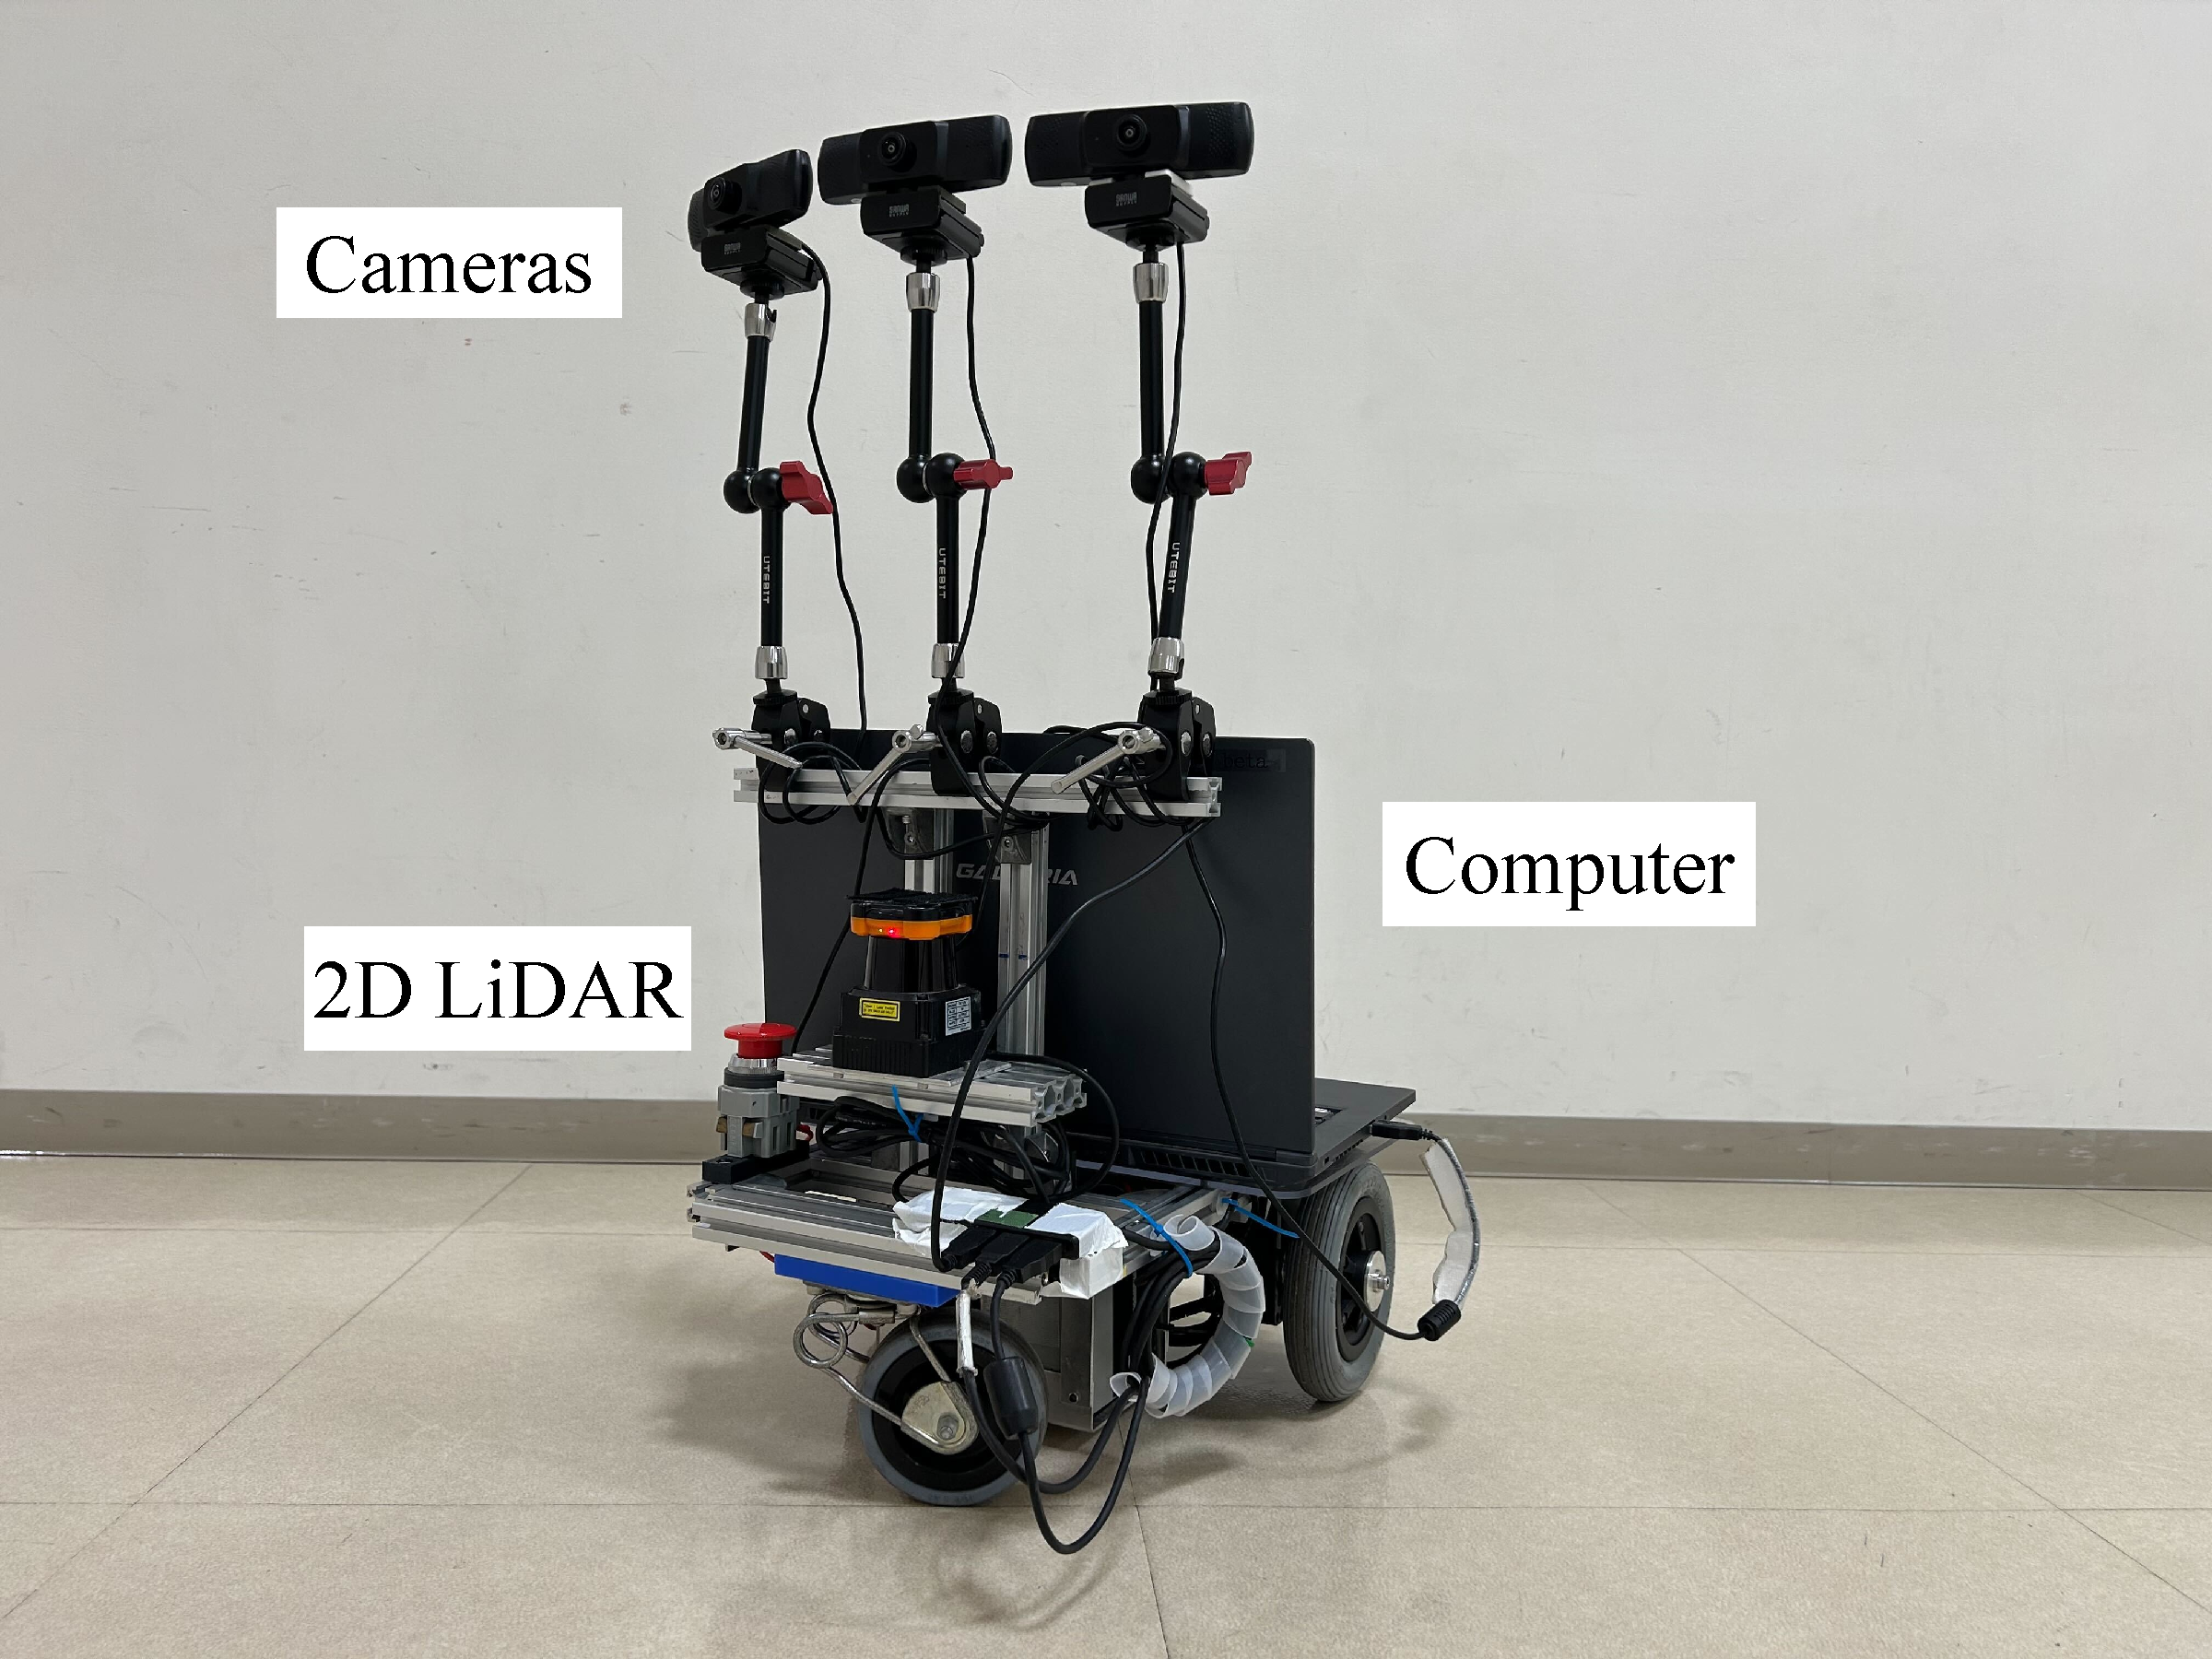
\includegraphics[width=60mm]{images/pdf/ishiguro/gamma.pdf}
     \caption{Experimental setup}
     \label{fig:gamma}
\end{figure}
\newpage
\section{実験方法}
\subsection{実験環境}
実験環境として\figref{fig:topo}に示す千葉工業大学 2 号館 3 階を用いる.
環境中には,三叉路が 6 つ,角が 3 つ,突き当りが 4 つ含まれている.
また,経路追従モジュールと通路分類モジュールの学習データを収集するために,\figref{fig:route}に示すルートを走行する.

\begin{figure}[htbp]
  \centering
  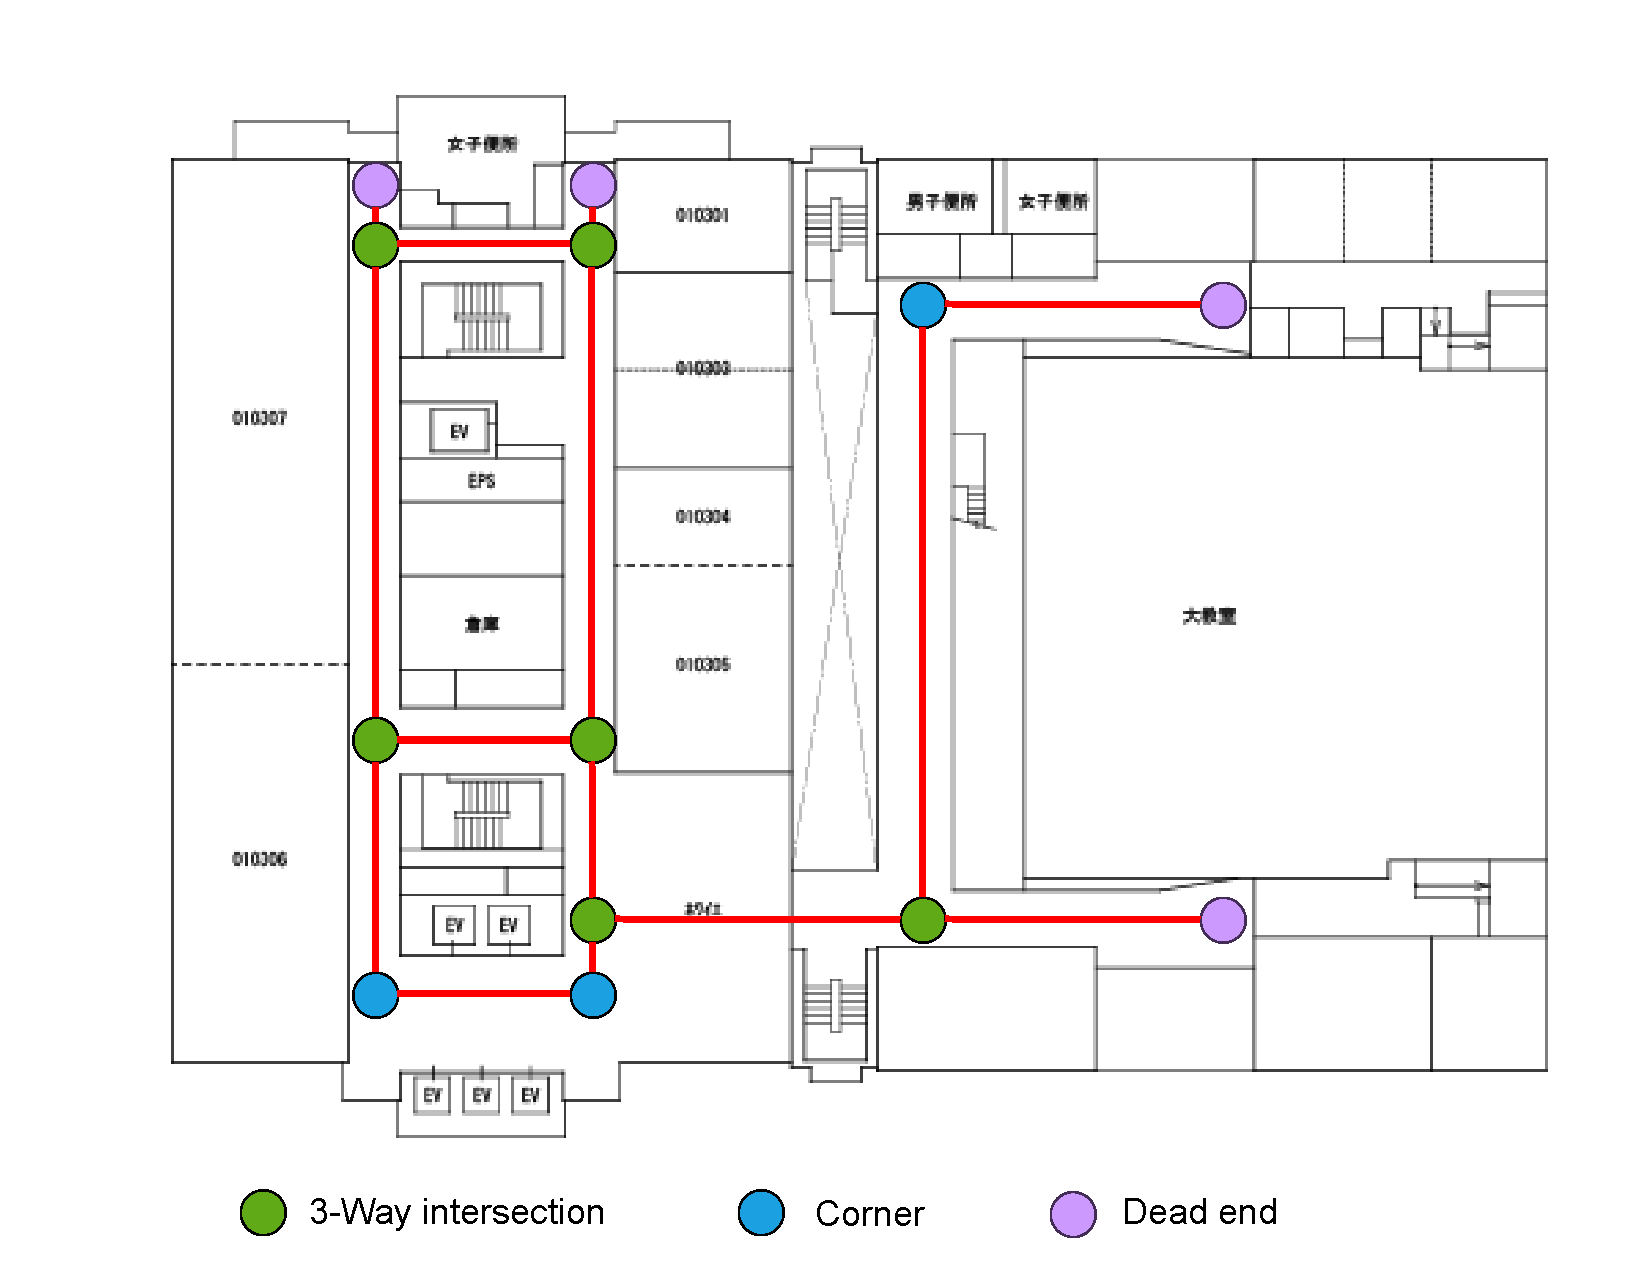
\includegraphics[width=130mm]{images/pdf/ishiguro/topo.pdf}
  \caption{Experimental environment}
  \label{fig:topo}
\end{figure}

\begin{figure}[h]
  \centering
  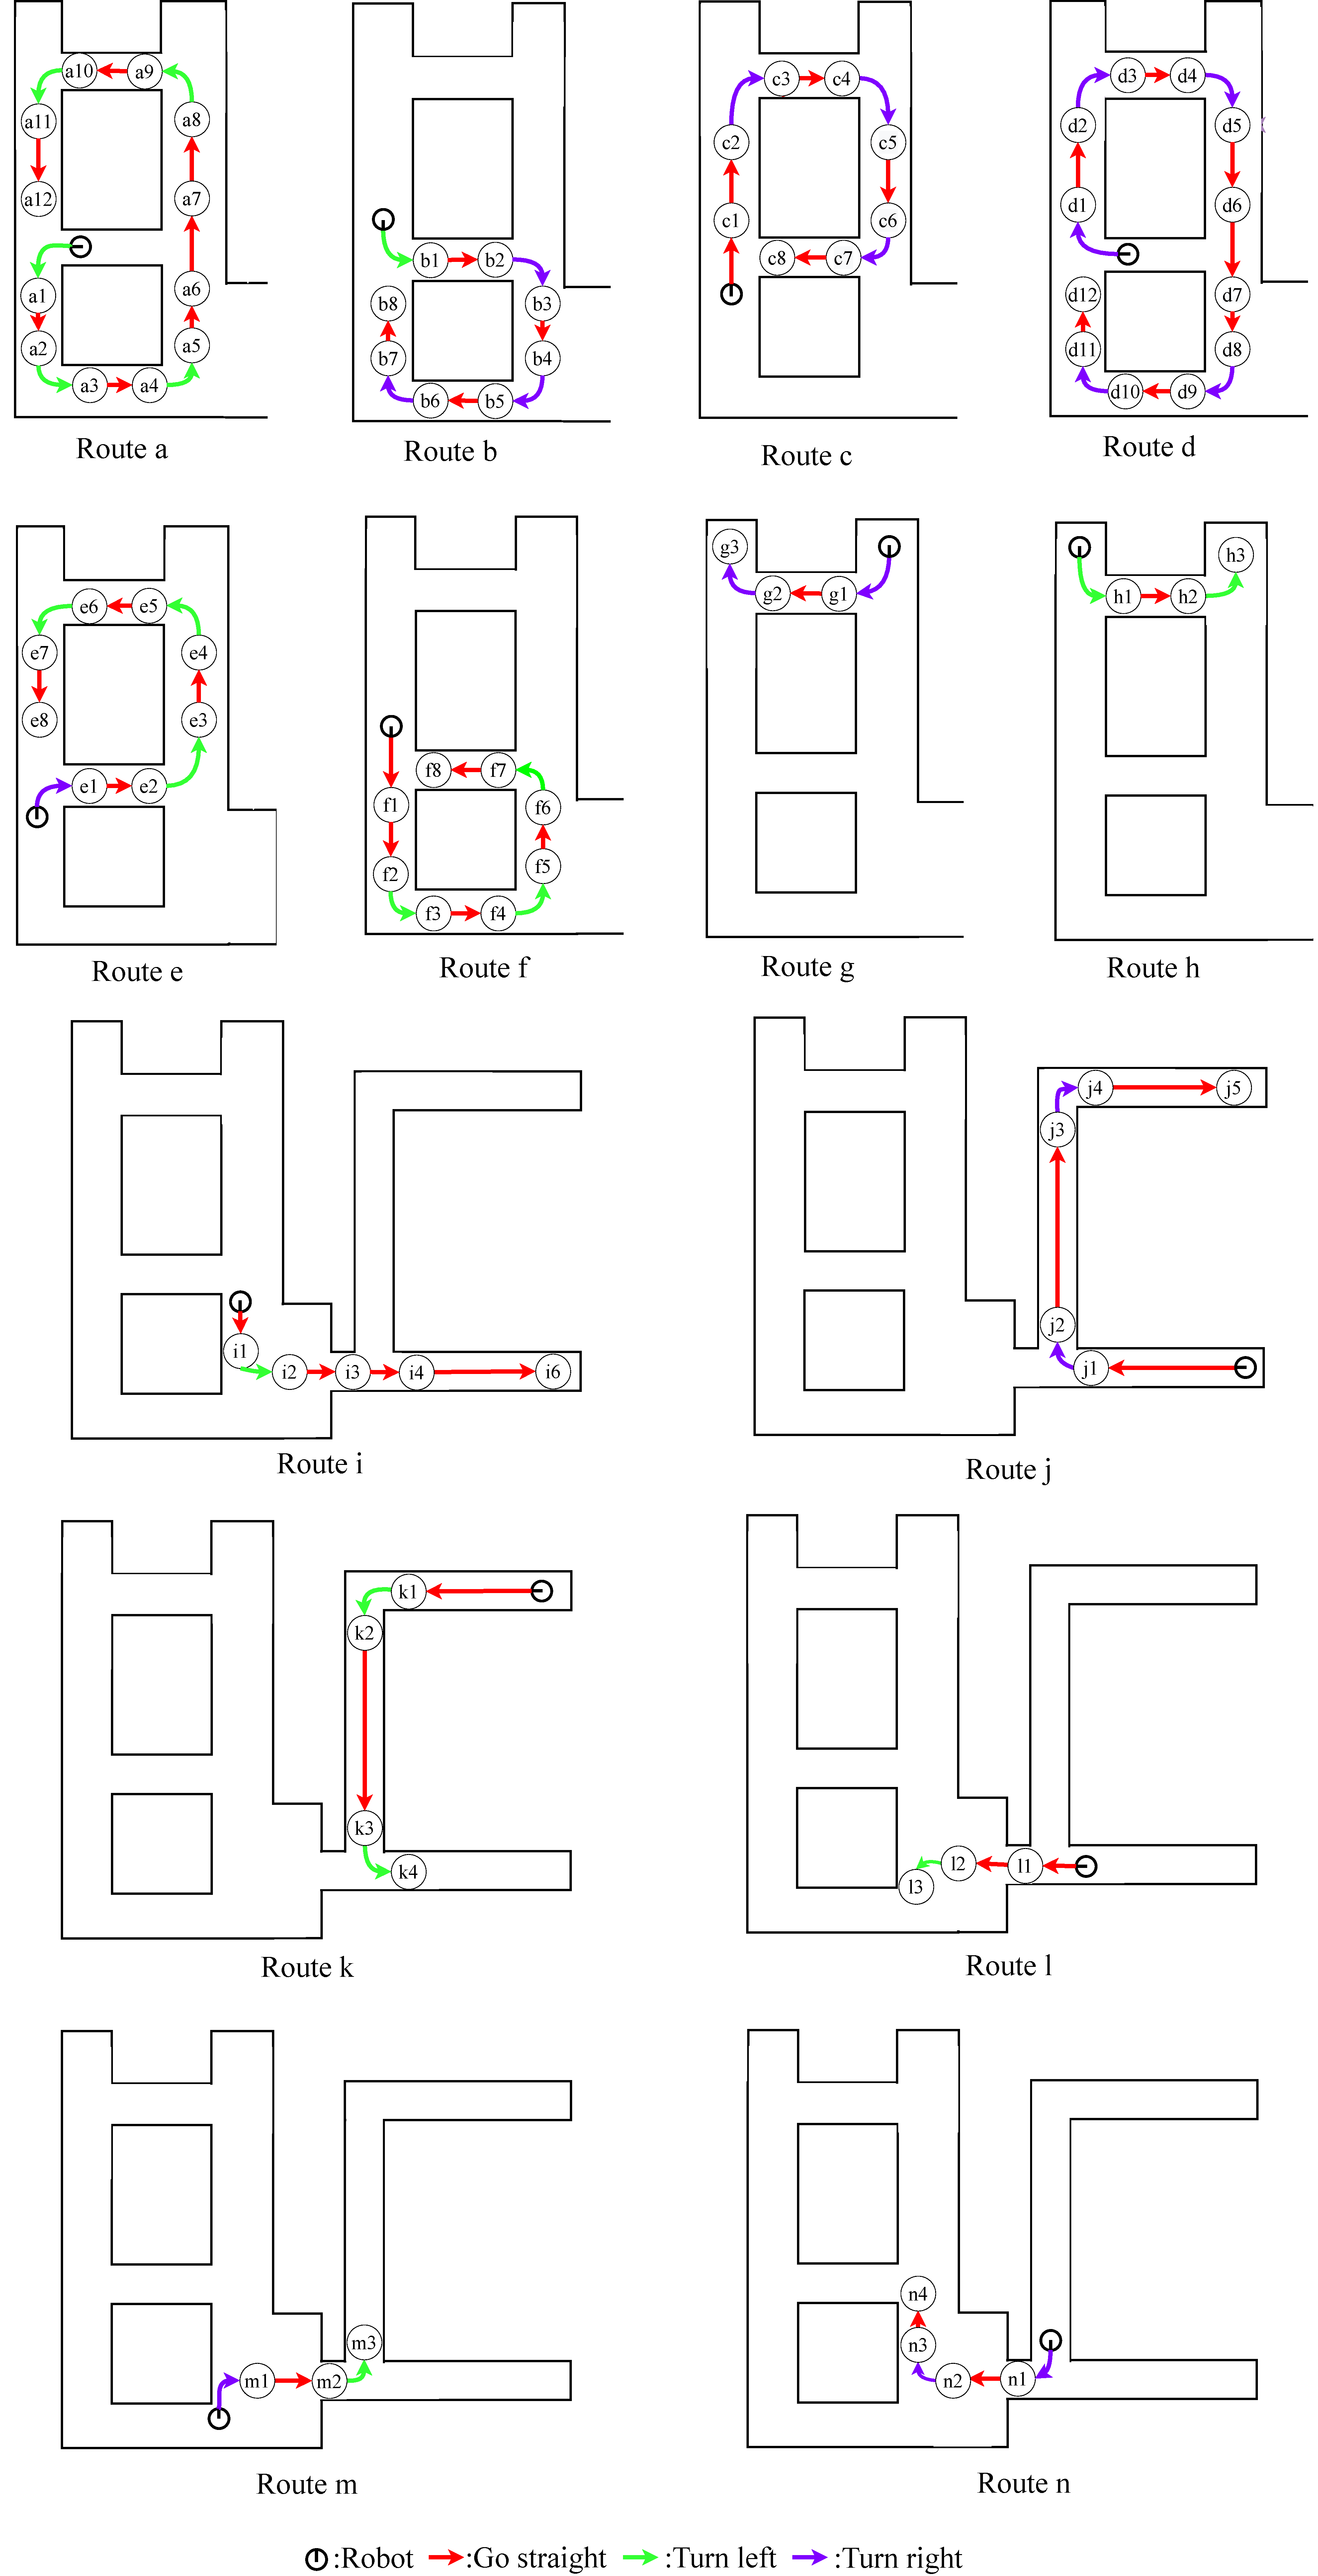
\includegraphics[width=100mm]{images/pdf/ishiguro/route.pdf}
  \caption{Route used for learning}
  \label{fig:route}
\end{figure}

\newpage
\subsection{シナリオの選定}
実験に使用するシナリオを,島田らが作成した 50 例から選定した.
選定するにあたって,以下の条件を設定した.

\begin{enumerate}
  \item [1)] ロボットが移動するには通路が狭すぎて,衝突せずに走行するのが困難な,\figref{fig:keepout}上部に示す部分を走行ルートに含まれないこと.
  \item [2)] 現時点の経路追従モジュールでは対応していない,「後ろを向く」などその場での旋回が含まれていないこと.
  % \item [3)] ロボットが移動しても,カメラ画像の特徴の変化が小さいため,通路の種類の分類が困難な\figref{fig:keepout}下部に示す部分がスタート地点では無いこと.
  \item [3)] スタート地点が\figref{fig:keepout}に示す箇所でないこと.この箇所がスタート地点のシナリオは,「左手に通路が見えるまで直進」か「右手に通路が見えるまで直進」である.現時点の路分類モジュールの入力である正面のカメラ画像からでは,ロボットが移動してもカメラ画像の特徴の変化が小さく,シナリオの条件を満たす通路分類結果が得られない可能性がある.
\end{enumerate}

条件ごとの除外したシナリオ数を\tabref{tab:remove}に示す.
また,条件 2 と 3 の両方を満たしたシナリオが 2 つある. 
これにより,選定されたシナリオ数は 28 例となる.
\begin{table}[htbp]
  \centering
  \caption{Number of scenarios excluded}\label{tab:remove}
  \begin{tabular}{c|c}
  \hline
  reason & number of secnario\\
  \hline
  1  & 4\\
  2  & 7\\
  3  & 13\\
  \hline
  \end{tabular}
\end{table}

\begin{figure}
  \centering
  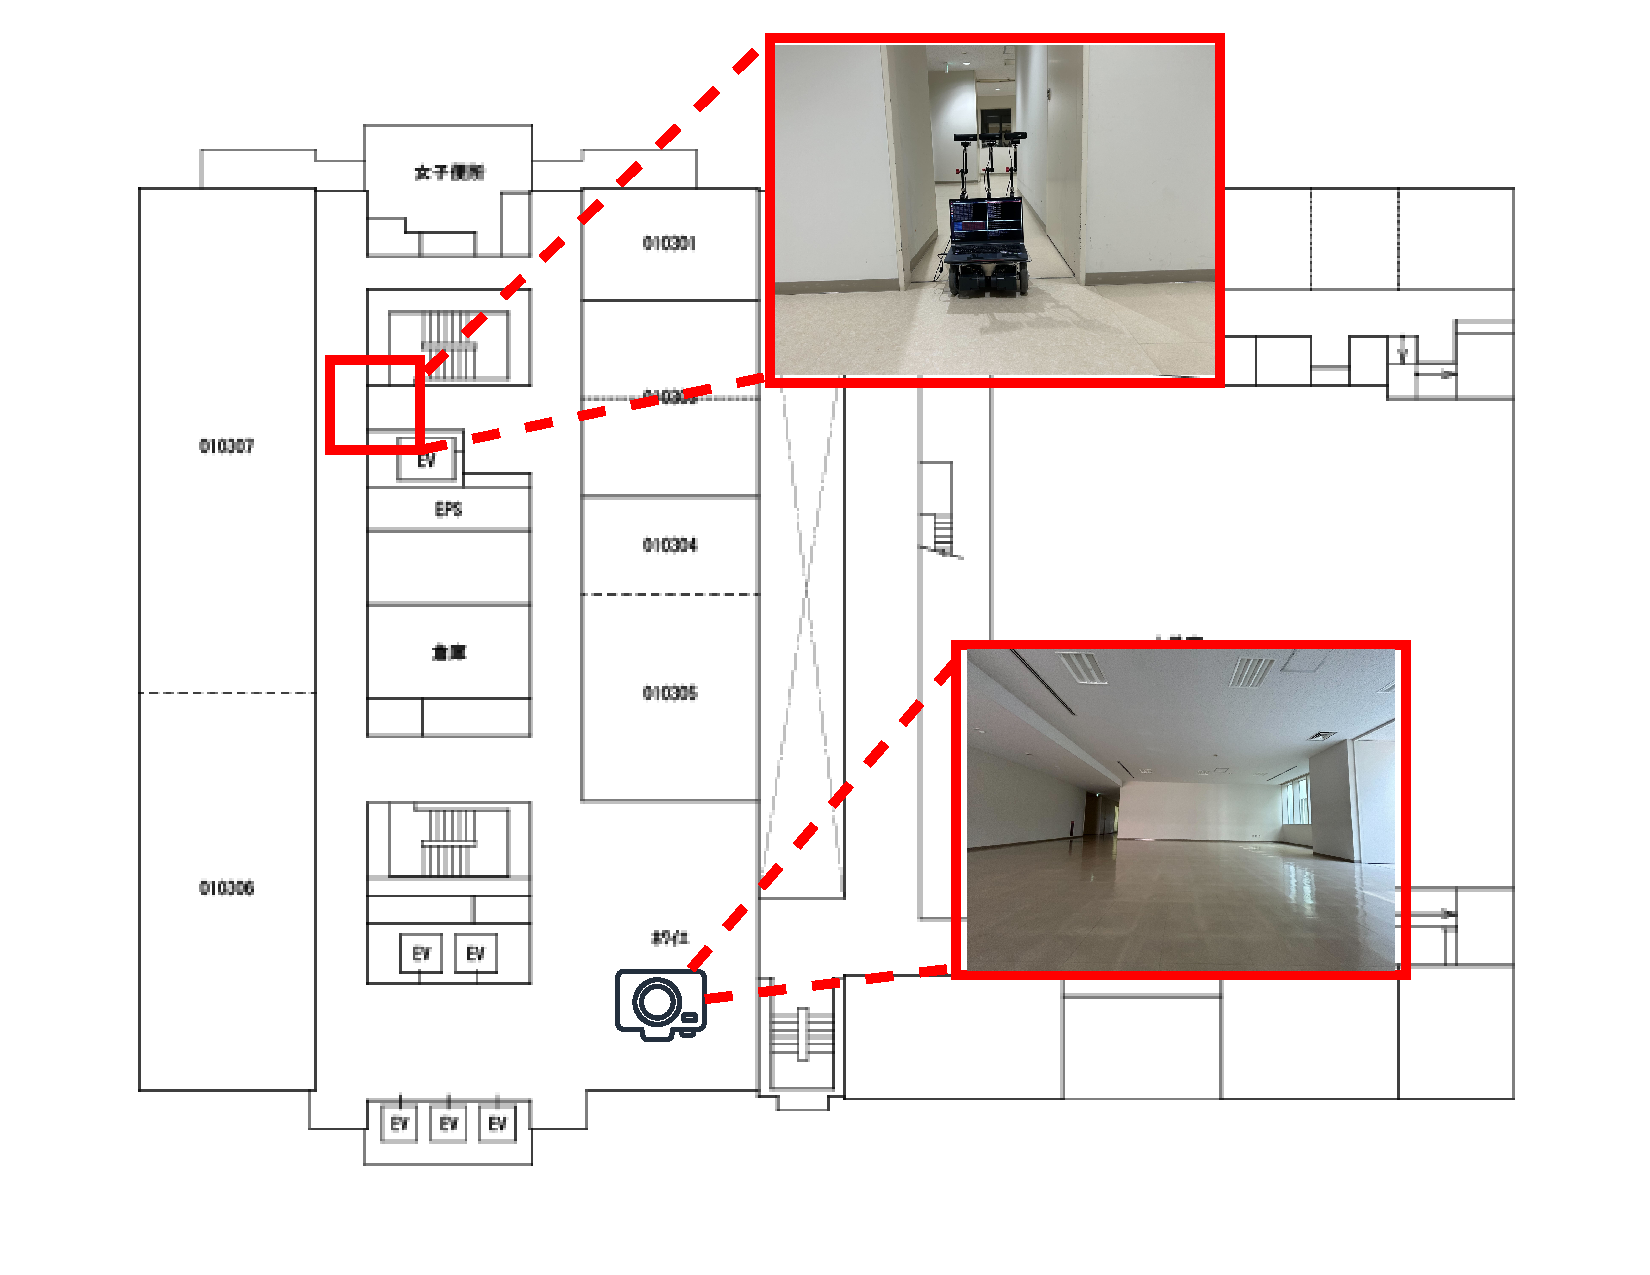
\includegraphics[width=130mm]{images/pdf/ishiguro/keepout.pdf}
  \caption{Excluded area for experiments}
  \label{fig:keepout}
\end{figure}

\clearpage
\subsection{経路追従モジュールの訓練}
\figref{fig:route}に示すルートをオンライン学習させながら 1 周走行する.
データセットの収集には藤原ら\cite{fujiwara2023}が提案する手法を用いる.
また,オンライン学習で作成したモデルに追加でオフライン学習を行う.
オフライン学習時のデータセットにはオンライン学習の際に作成したルート 1 周分のデータを用いる.
データセットからはオンライン学習と同様のバッチサイズ 8 でデータをランダムに取得し,epoch数は 20 とした.

\subsection{通路分類モジュールの訓練}
\figref{fig:route}に示すルートをROS の navigation パッケージを使用して,経路を 1 周する.
その際, 3 つのカメラからそれぞれ画像データを収集しながら走行する.
学習時のパラメータとして,バッチサイズを 32 ,epoch数を 30 とし,コストアプローチに用いた重みは\tabref{tab:cost}に示す.

\begin{table}[htbp]
  \centering
  \caption{The weights assigned to each class in the experiment}\label{tab:cost}
  \begin{tabular}{c|c}
  \hline
  Class & Class weights\\
  \hline
  直進   & 1\\
  突き当たり   & 39.5\\
  角(右) & 14\\
  角(左)& 14.2 \\
  十字路 & 1  \\
  三叉路(右)& 6.6  \\
  三叉路(中央)& 7.0  \\
  三叉路(左) & 6.4  \\
  \hline
  \end{tabular}
\end{table}

\clearpage
\subsection{シナリオに基づくナビゲーション}
2 つのモジュールを訓練後,ロボットが目的地まで到達できるか確認する.
実験では,ロボットをシナリオのスタート地点,向きに配置し,シナリオを 1 例ずつ入力する.
壁に衝突することなく正しい経路を選択し,目的地で停止した場合に成功とする.
\chapter{おわりに}
\label{chap:end}
\section{結論}
本論文では,春山らが提案したシステムを改良し,先行研究では走行が未確認であったシナリオに対しても目的地までカメラ画像のみを入力として経路追従可能か検証した.
経路追従の成功率を向上させることを目的として,先行研究からは,行動ごとにモデルを切り替えるネットワークに変更,オフライン学習による追学習する仕組みを追加した.
また,これらの手法が経路追従の成功率を向上させることを,シミュレータでの実験で検証した.
実ロボットを用いた実験では,先行研究では走行が確認されていないエリアをシナリオを含む場合でも 28 例中,24例は目的地まで経路追従が可能であること確認した.
失敗した4例に関して,通路分類モジュールの出力が遅れることによって,経路追従に失敗すると考えられる.

%
%% Back Matter
\backmatter{}
%
%!TEX root = ../thesis.tex
%\bibliographystyle{plain}
\bibliographystyle{junsrt}
%\bibliography{report}
\nocite{*}
\bibliography{main_bibliography}
%
% %!TEX root = ../thesis.tex
\chapter*{付録}
\addcontentsline{toc}{chapter}{付録}
実験に使用したシナリオを掲載する.

\begin{figure*}[htbp]
  \begin{tabular}{cc}
      \begin{minipage}[t]{0.48\textwidth}
          \centering
          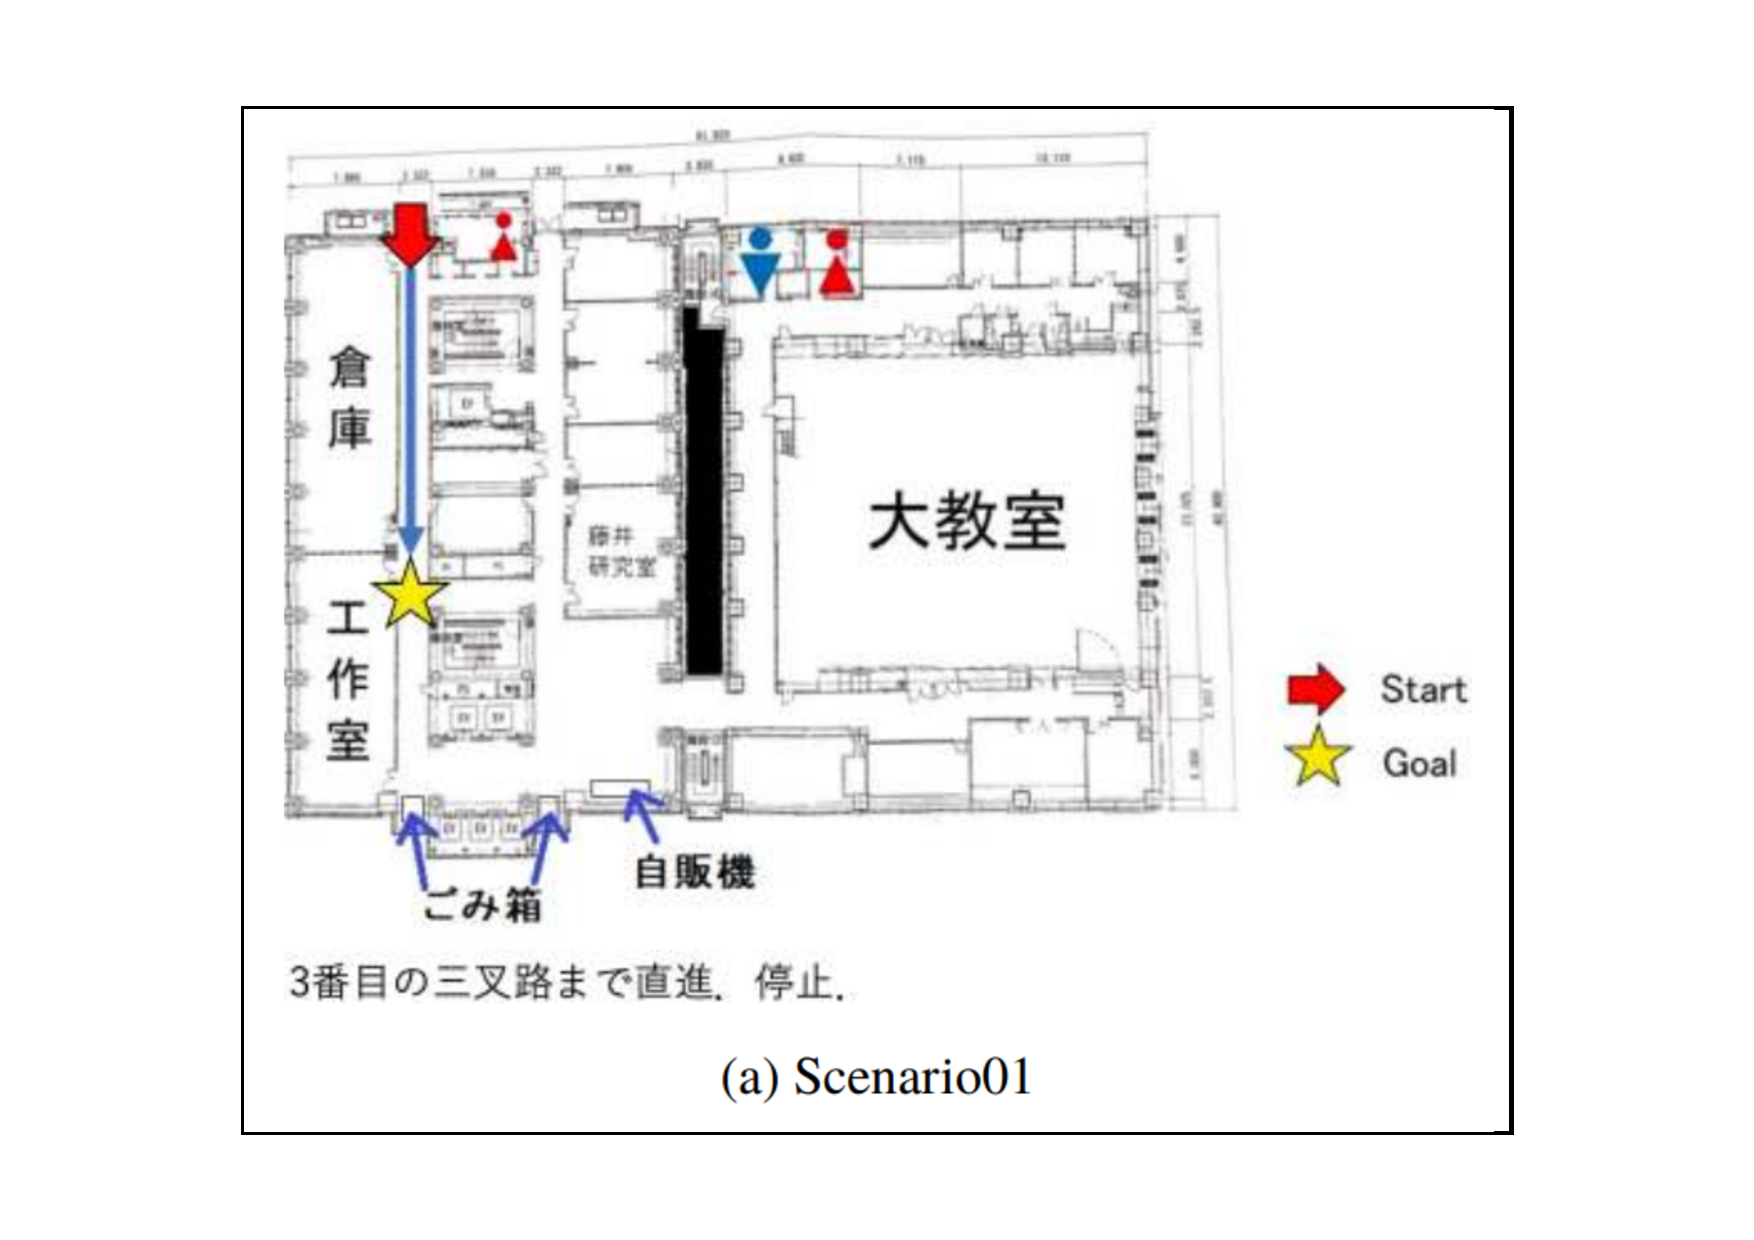
\includegraphics[keepaspectratio, width=80mm]{images/pdf/ishiguro/scenario/1.pdf}
          \subcaption{scenario01}
      \end{minipage} &
      \begin{minipage}[t]{0.48\textwidth}
          \centering
          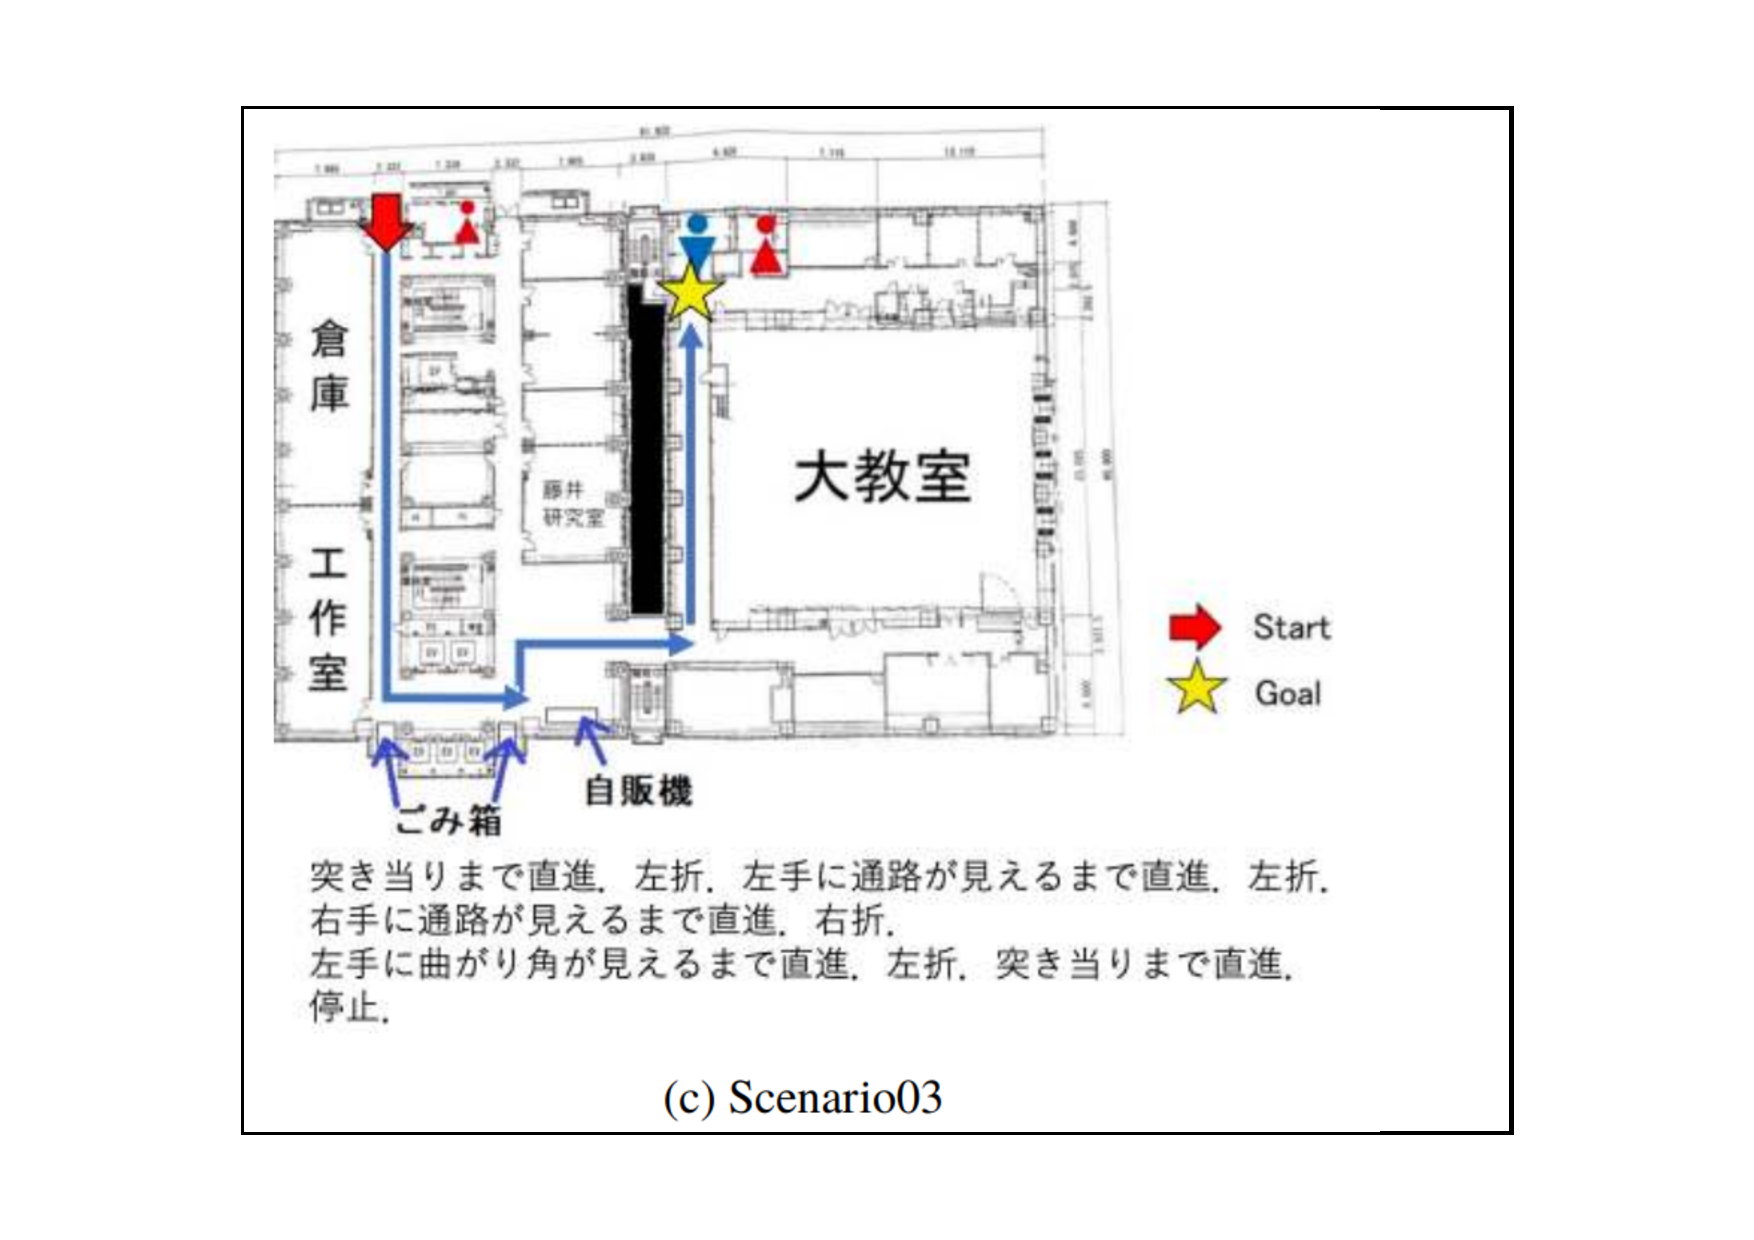
\includegraphics[keepaspectratio, width=80mm]{images/pdf/ishiguro/scenario/3.pdf}
          \subcaption{scenario03}
      \end{minipage} \\
      \begin{minipage}[t]{0.48\textwidth}
        \centering
        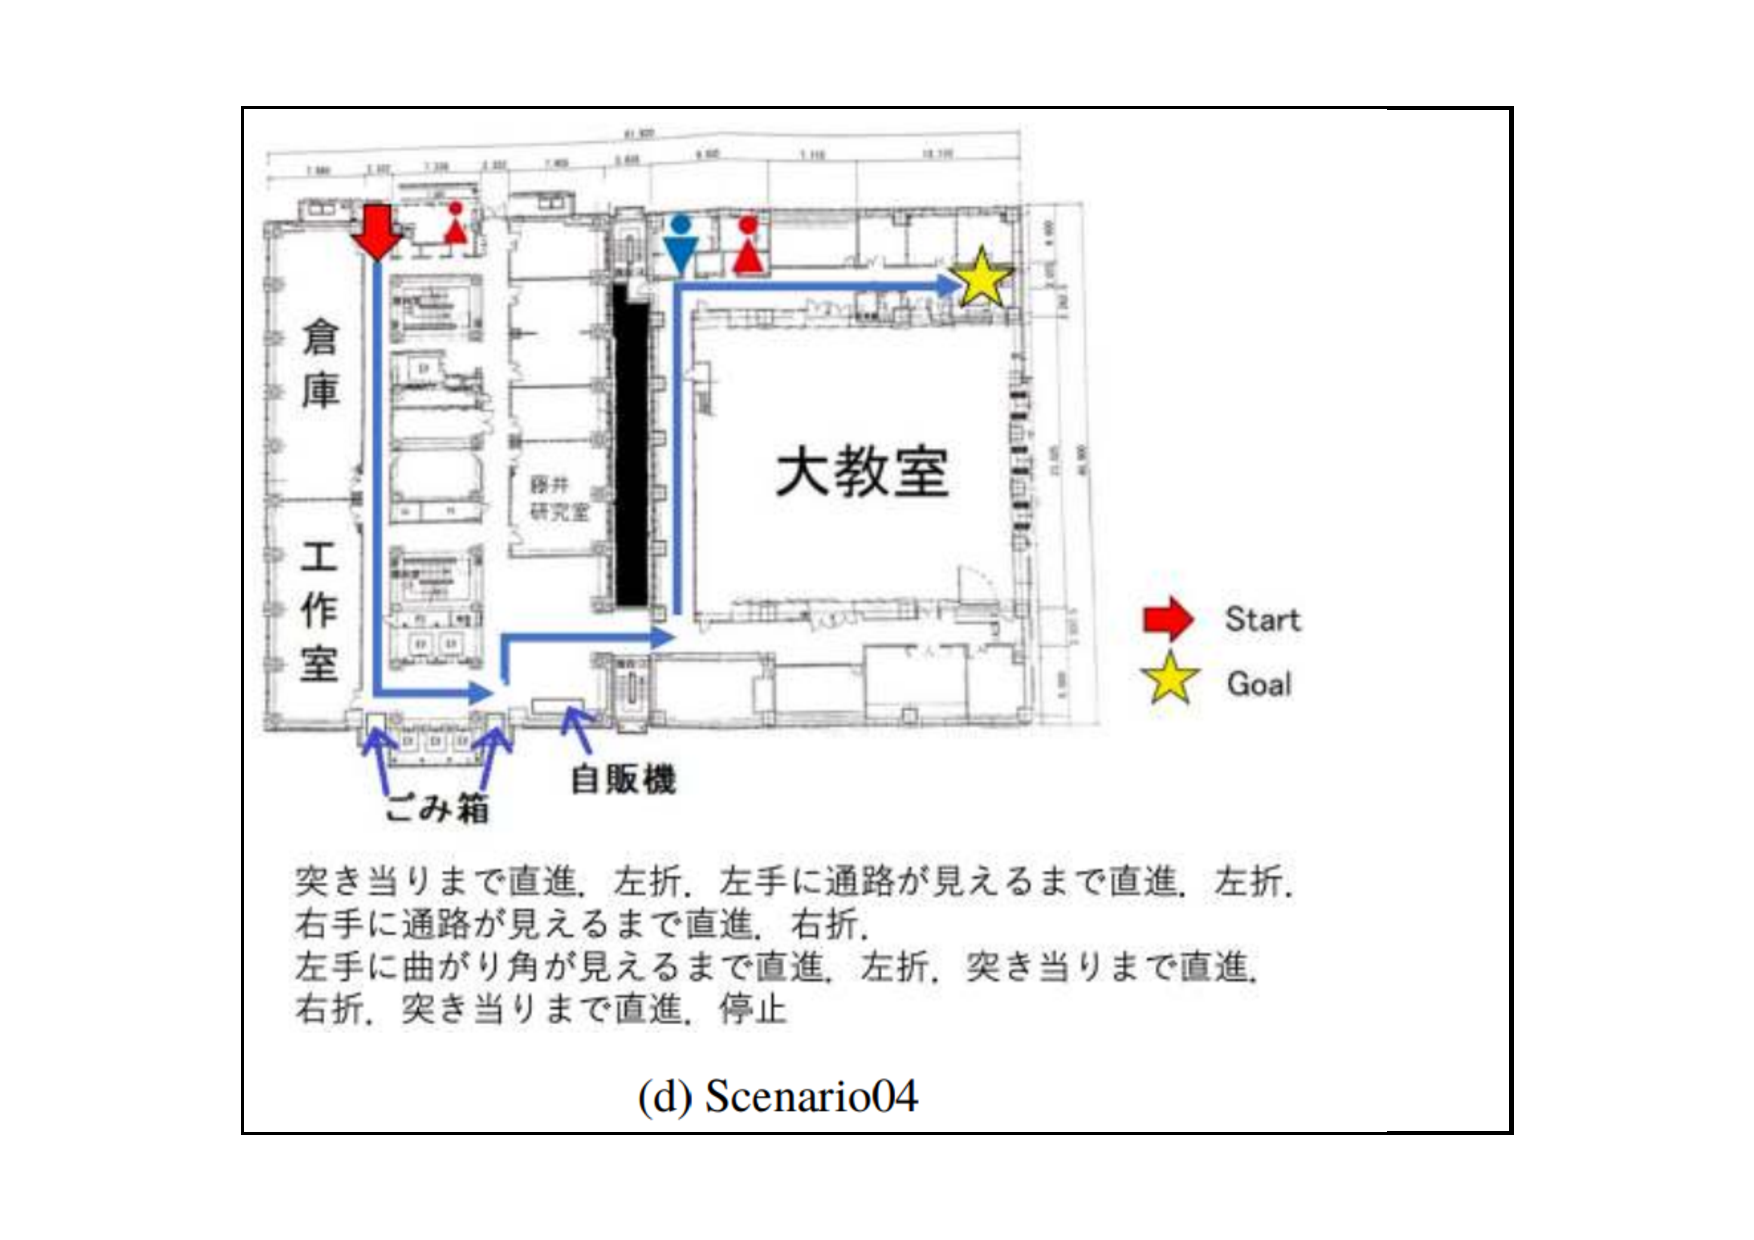
\includegraphics[keepaspectratio, width=80mm]{images/pdf/ishiguro/scenario/4.pdf}
        \subcaption{scenario05}
      \end{minipage} &
      \begin{minipage}[t]{0.48\textwidth}
        \centering
        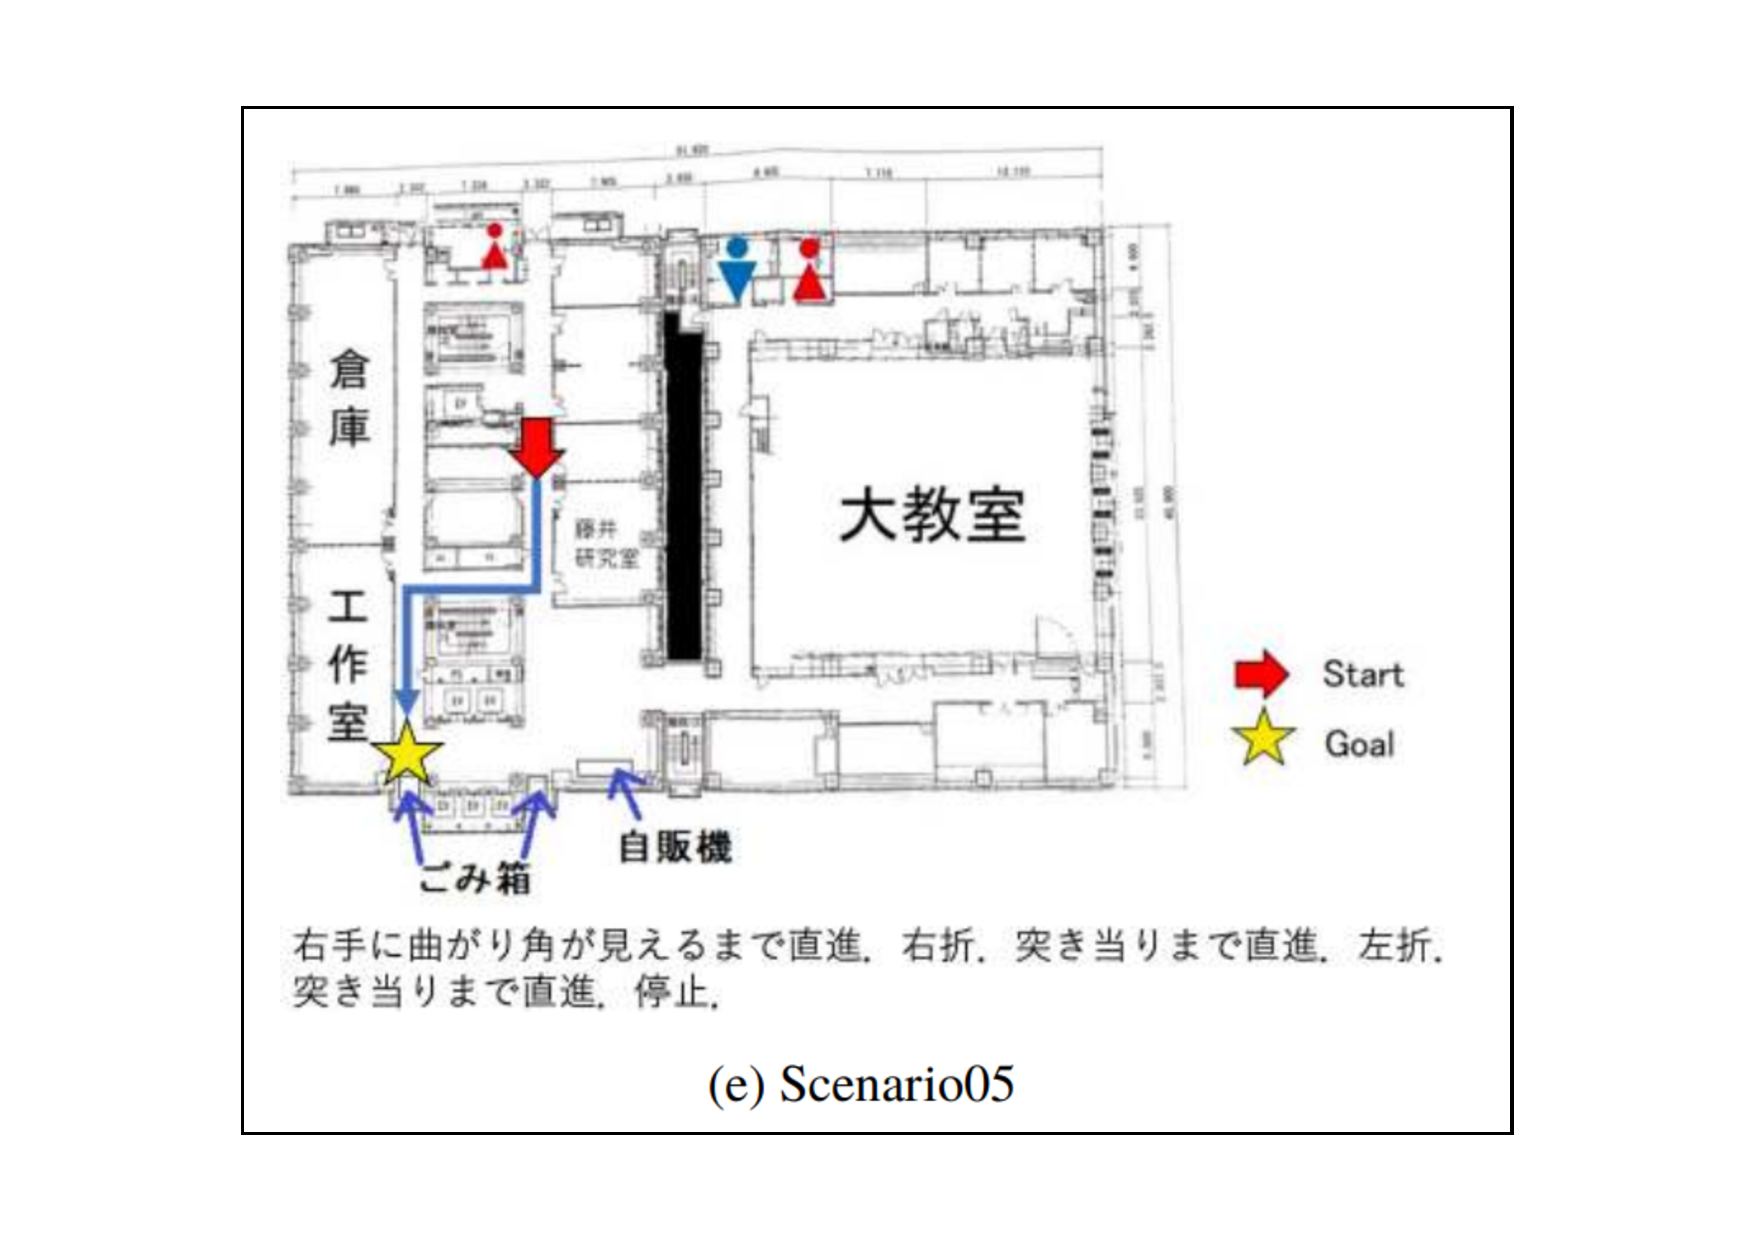
\includegraphics[keepaspectratio, width=80mm]{images/pdf/ishiguro/scenario/5.pdf}
        \subcaption{scenario06}
      \end{minipage} \\
      \begin{minipage}[t]{0.48\textwidth}
        \centering
        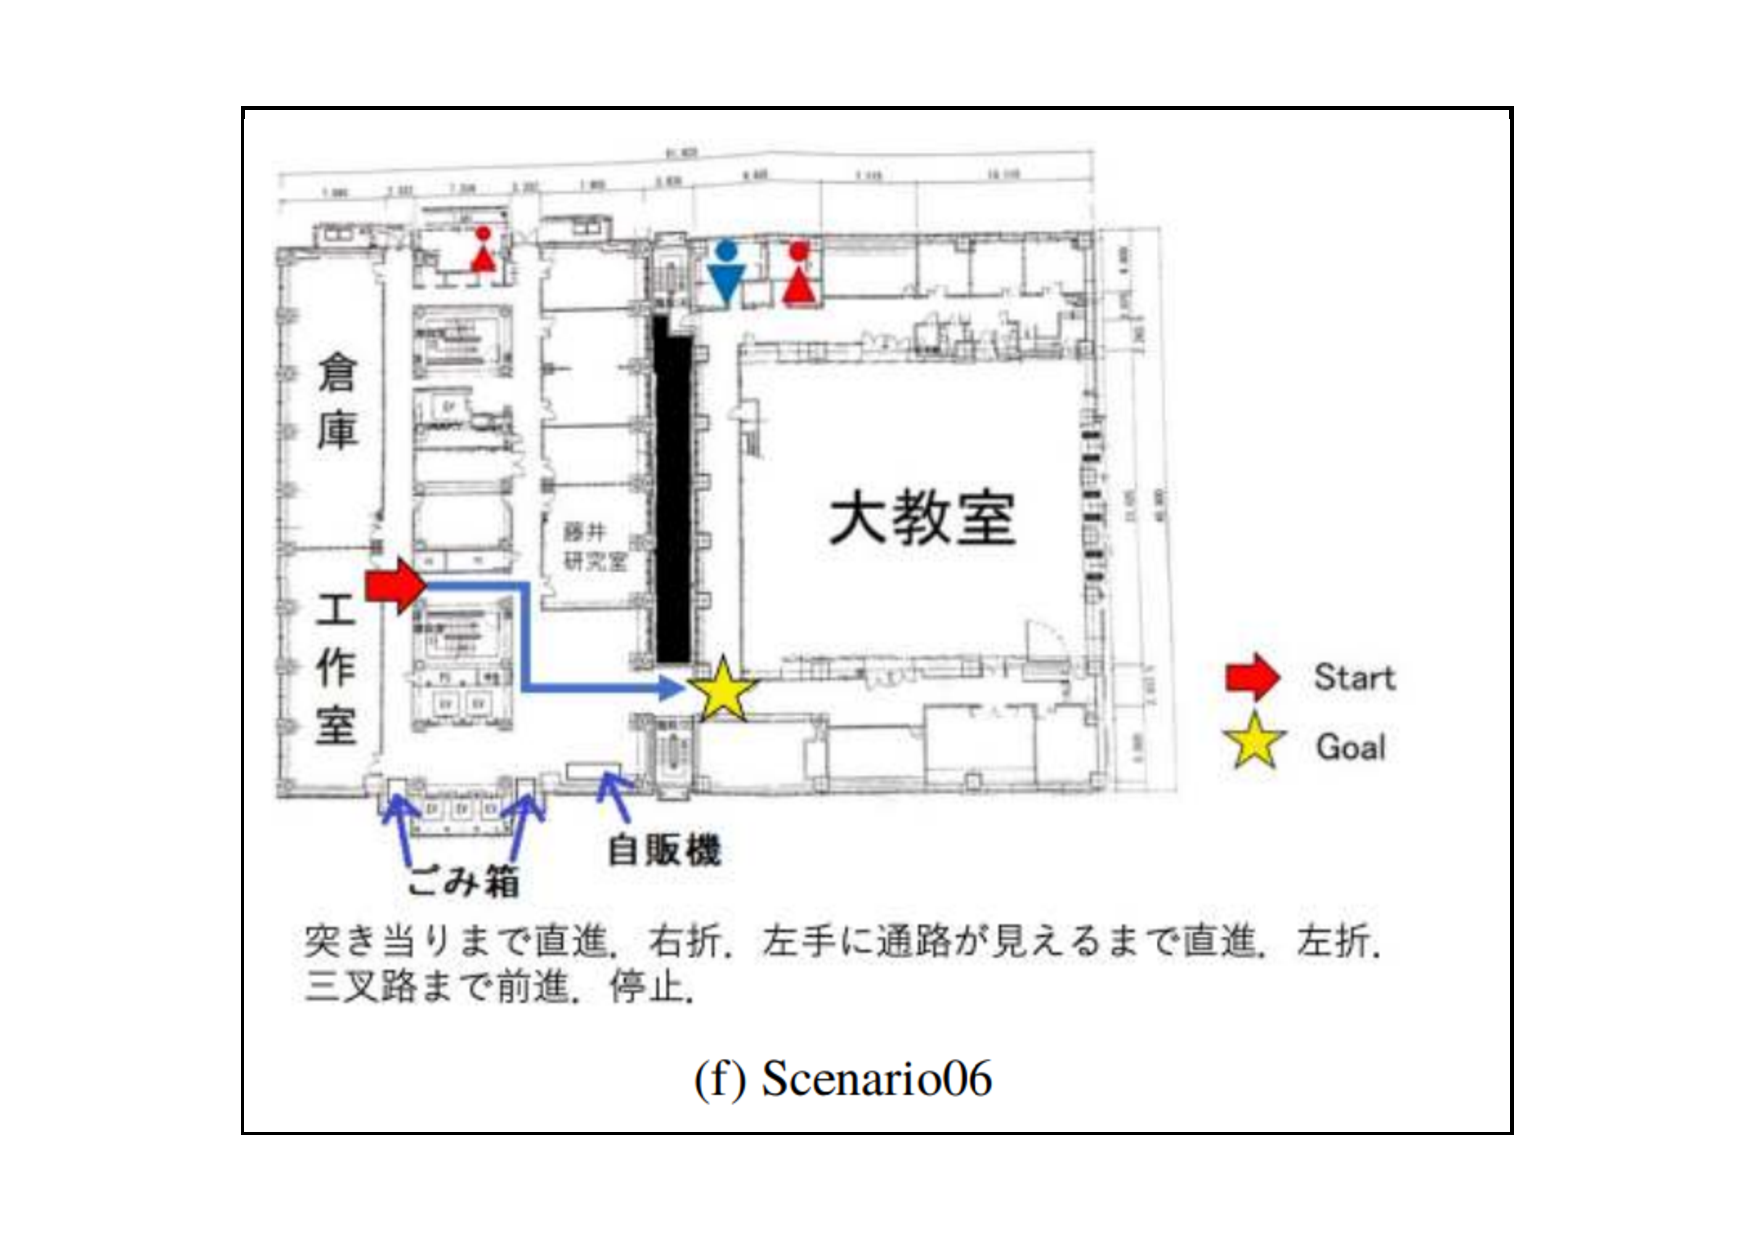
\includegraphics[keepaspectratio, width=80mm]{images/pdf/ishiguro/scenario/6.pdf}
        \subcaption{scenario06}
      \end{minipage} &
      \begin{minipage}[t]{0.48\textwidth}
        \centering
        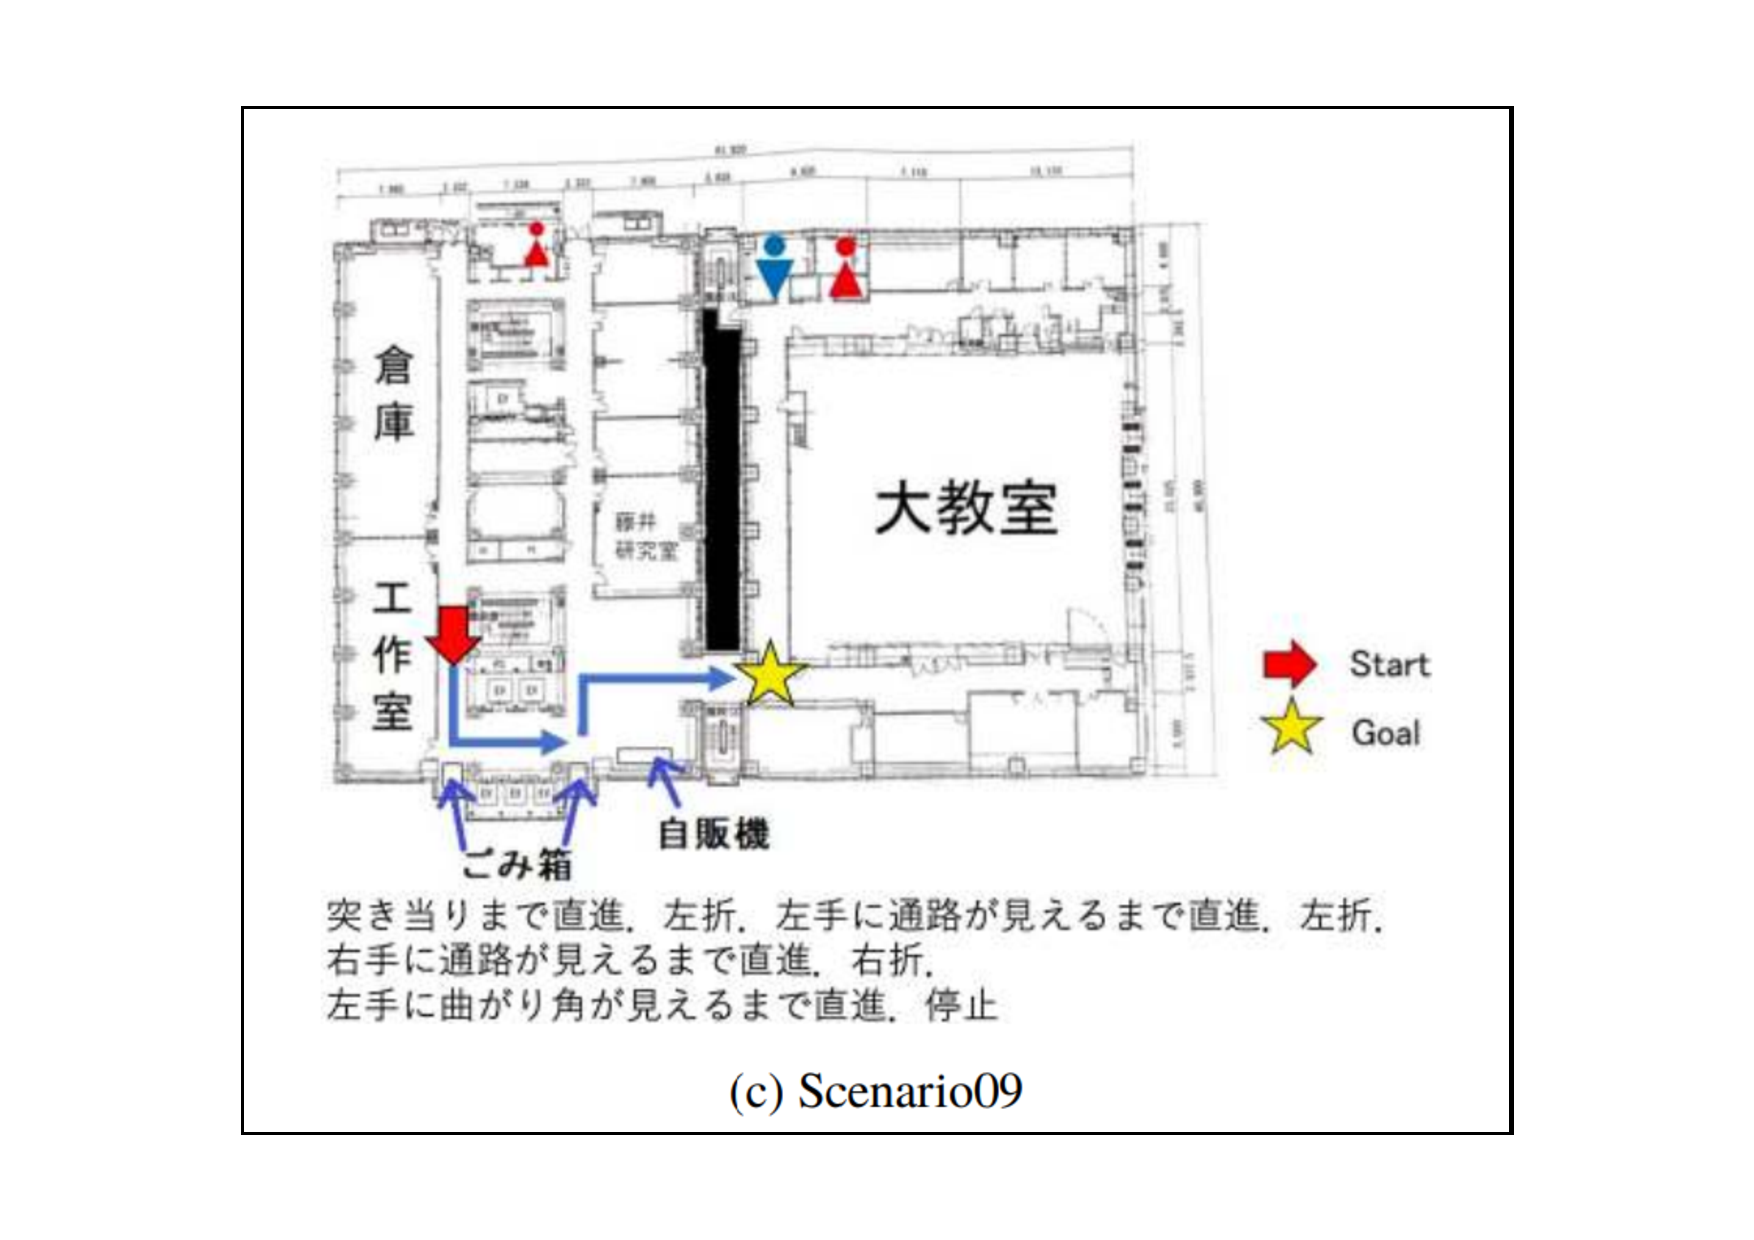
\includegraphics[keepaspectratio, width=80mm]{images/pdf/ishiguro/scenario/9.pdf}
        \subcaption{scenario09}
      \end{minipage}
  \end{tabular}
\caption{Scenarios 01 to 09}
\label{fig:scenario_1_9}
\end{figure*}

\begin{figure*}[htbp]
  \begin{tabular}{cc}
      \begin{minipage}[t]{0.48\textwidth}
        \centering
        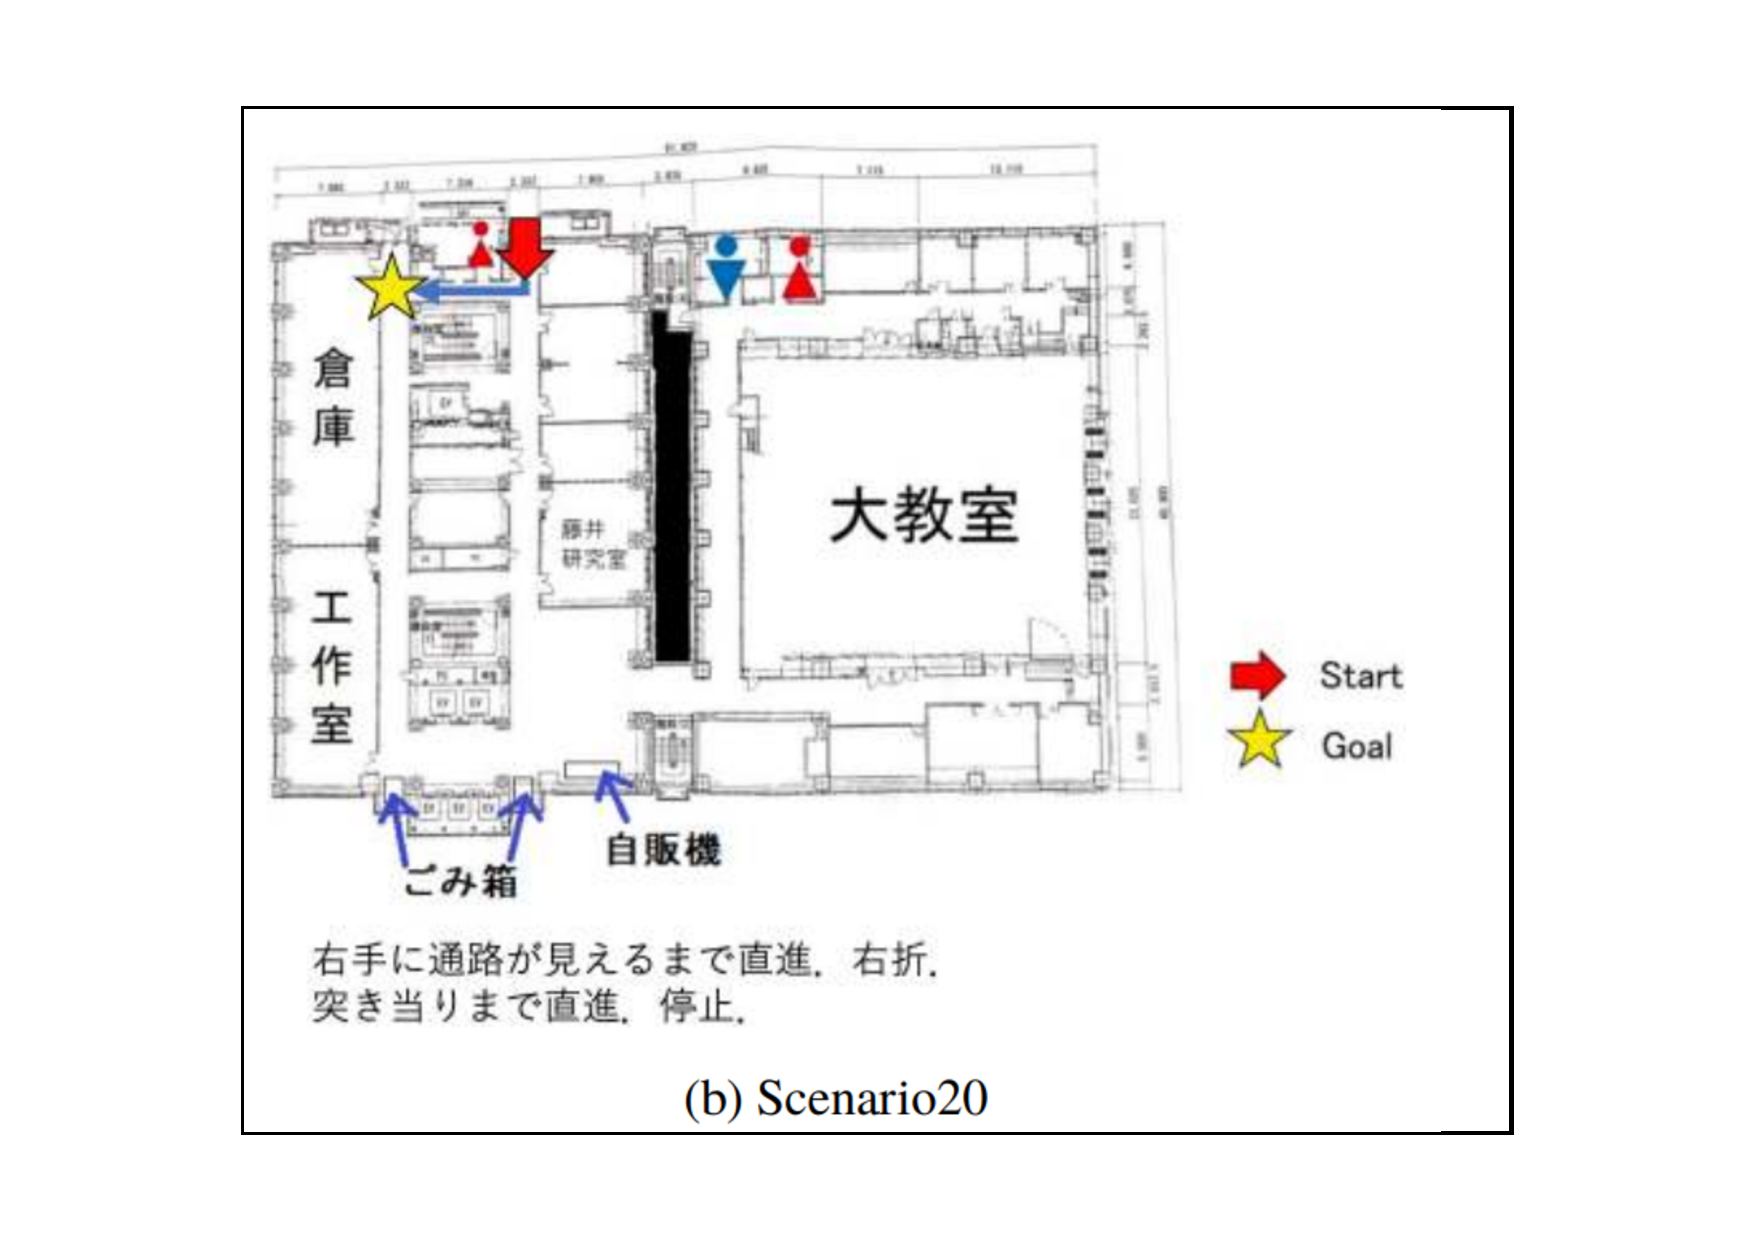
\includegraphics[keepaspectratio, width=80mm]{images/pdf/ishiguro/scenario/20.pdf}
        \subcaption{scenario20}
      \end{minipage} &
      \begin{minipage}[t]{0.48\textwidth}
        \centering
        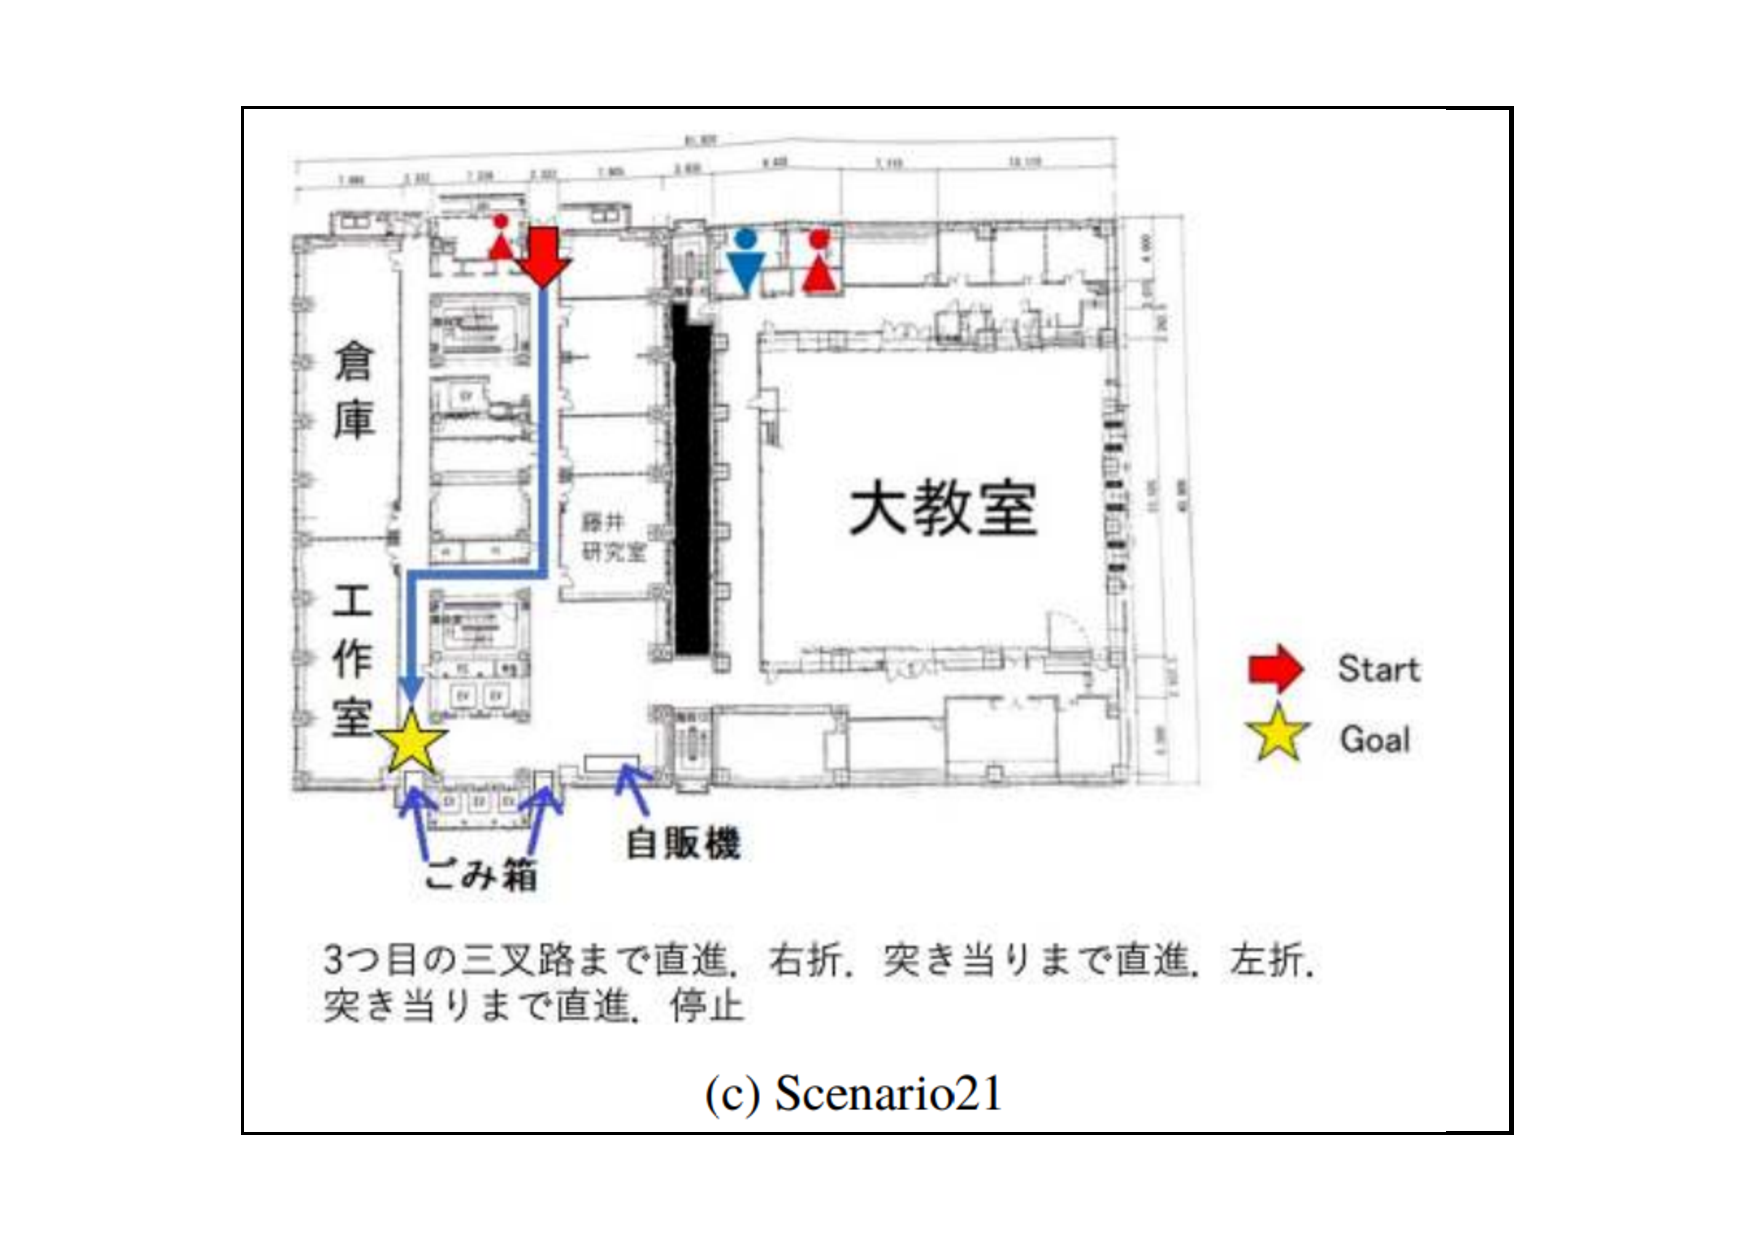
\includegraphics[keepaspectratio, width=80mm]{images/pdf/ishiguro/scenario/21.pdf}
        \subcaption{scenario21}
      \end{minipage} \\
      \begin{minipage}[t]{0.48\textwidth}
        \centering
        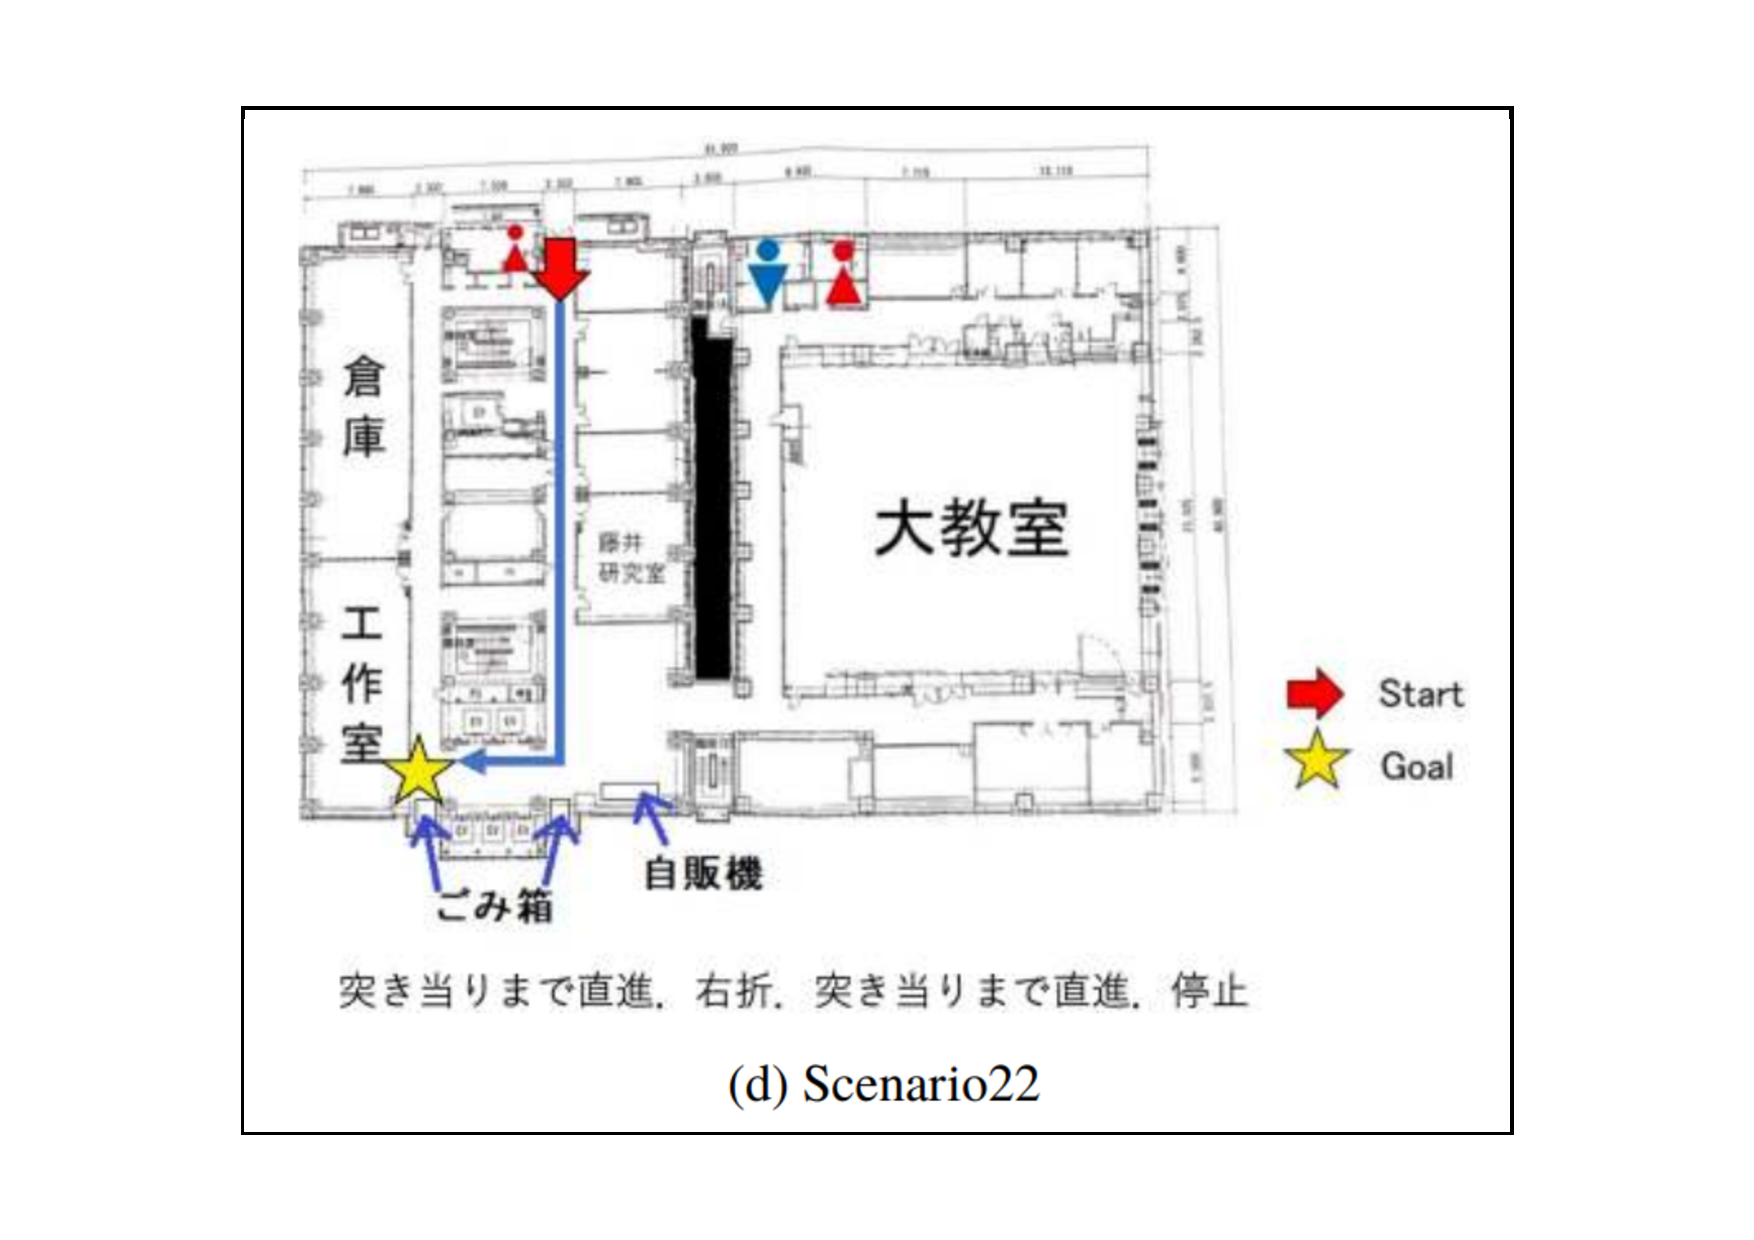
\includegraphics[keepaspectratio, width=80mm]{images/pdf/ishiguro/scenario/22.pdf}
        \subcaption{scenario22}
      \end{minipage} &
      \begin{minipage}[t]{0.48\textwidth}
        \centering
        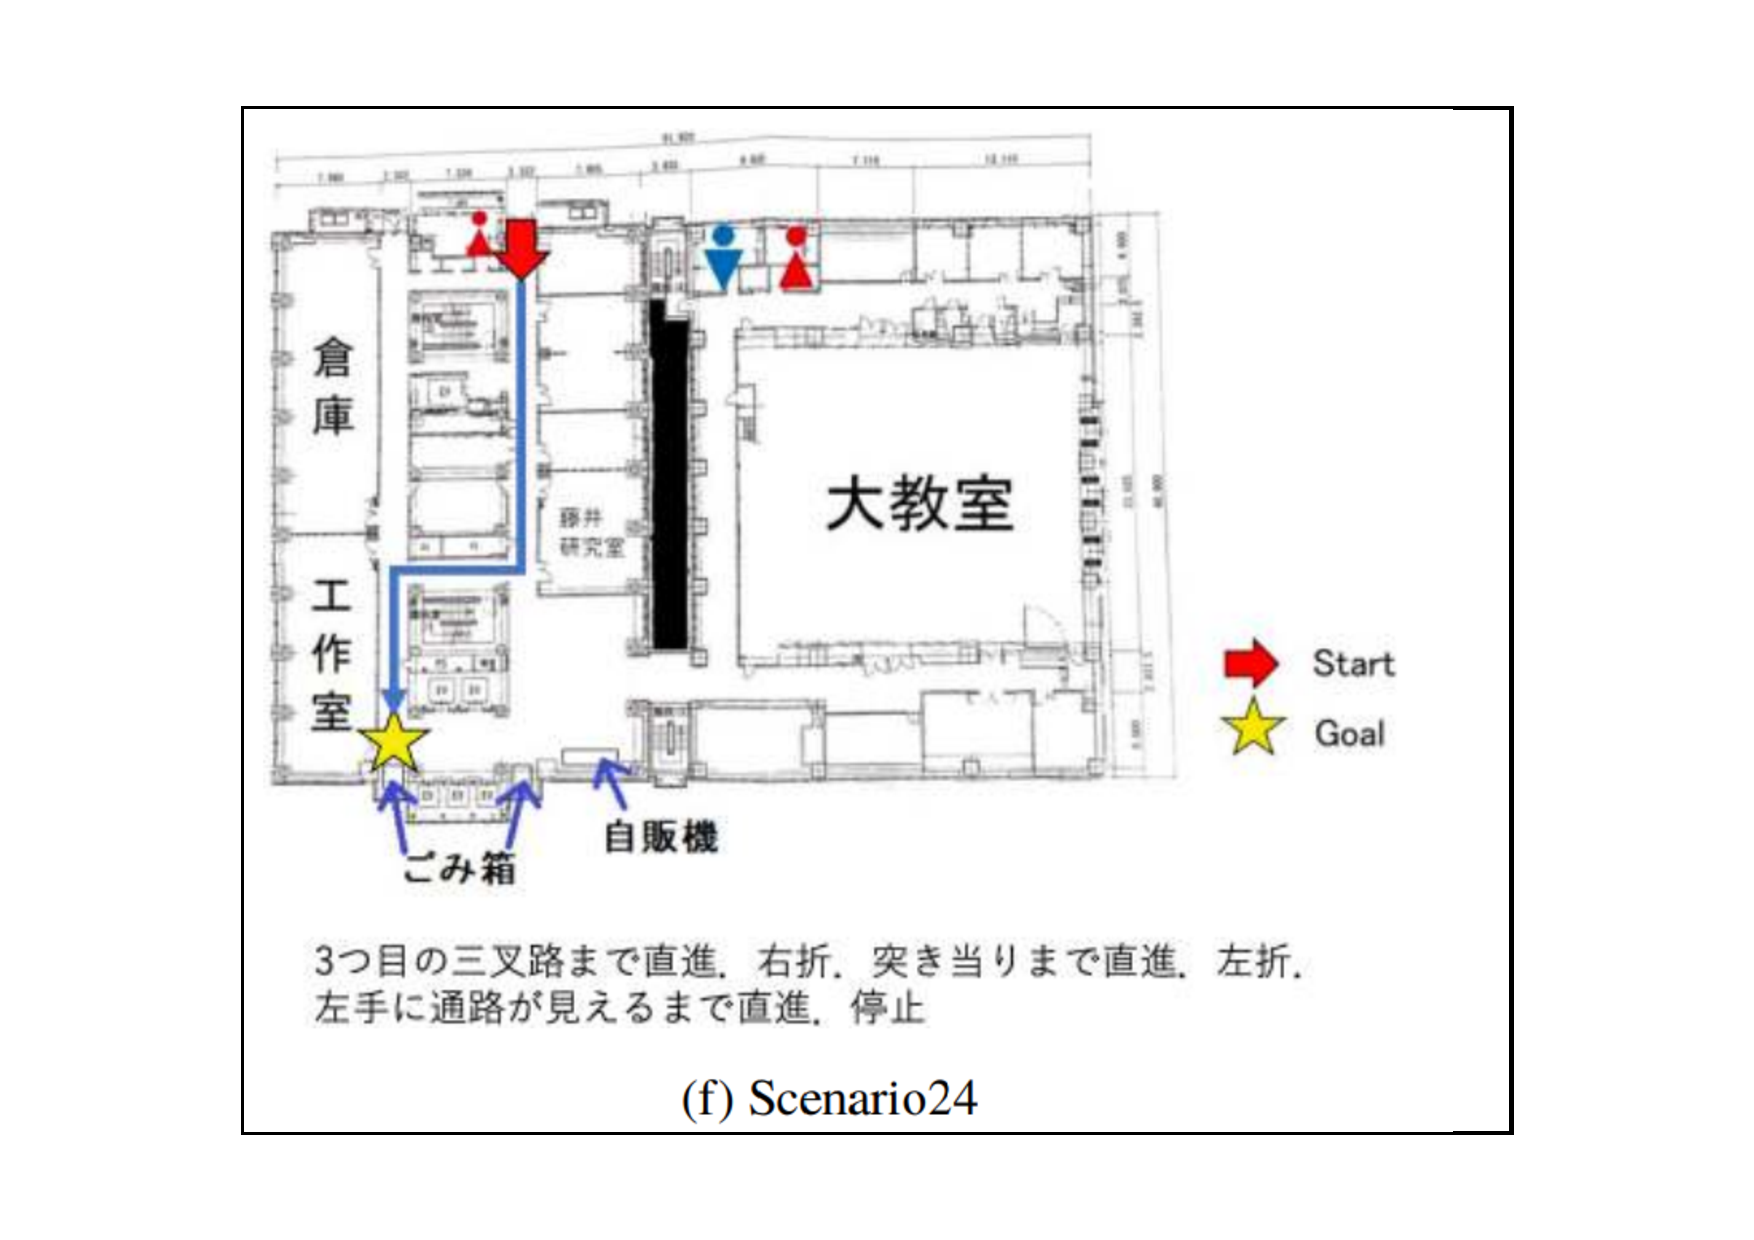
\includegraphics[keepaspectratio, width=80mm]{images/pdf/ishiguro/scenario/24.pdf}
        \subcaption{scenario24}
      \end{minipage} \\
      \begin{minipage}[t]{0.48\textwidth}
        \centering
        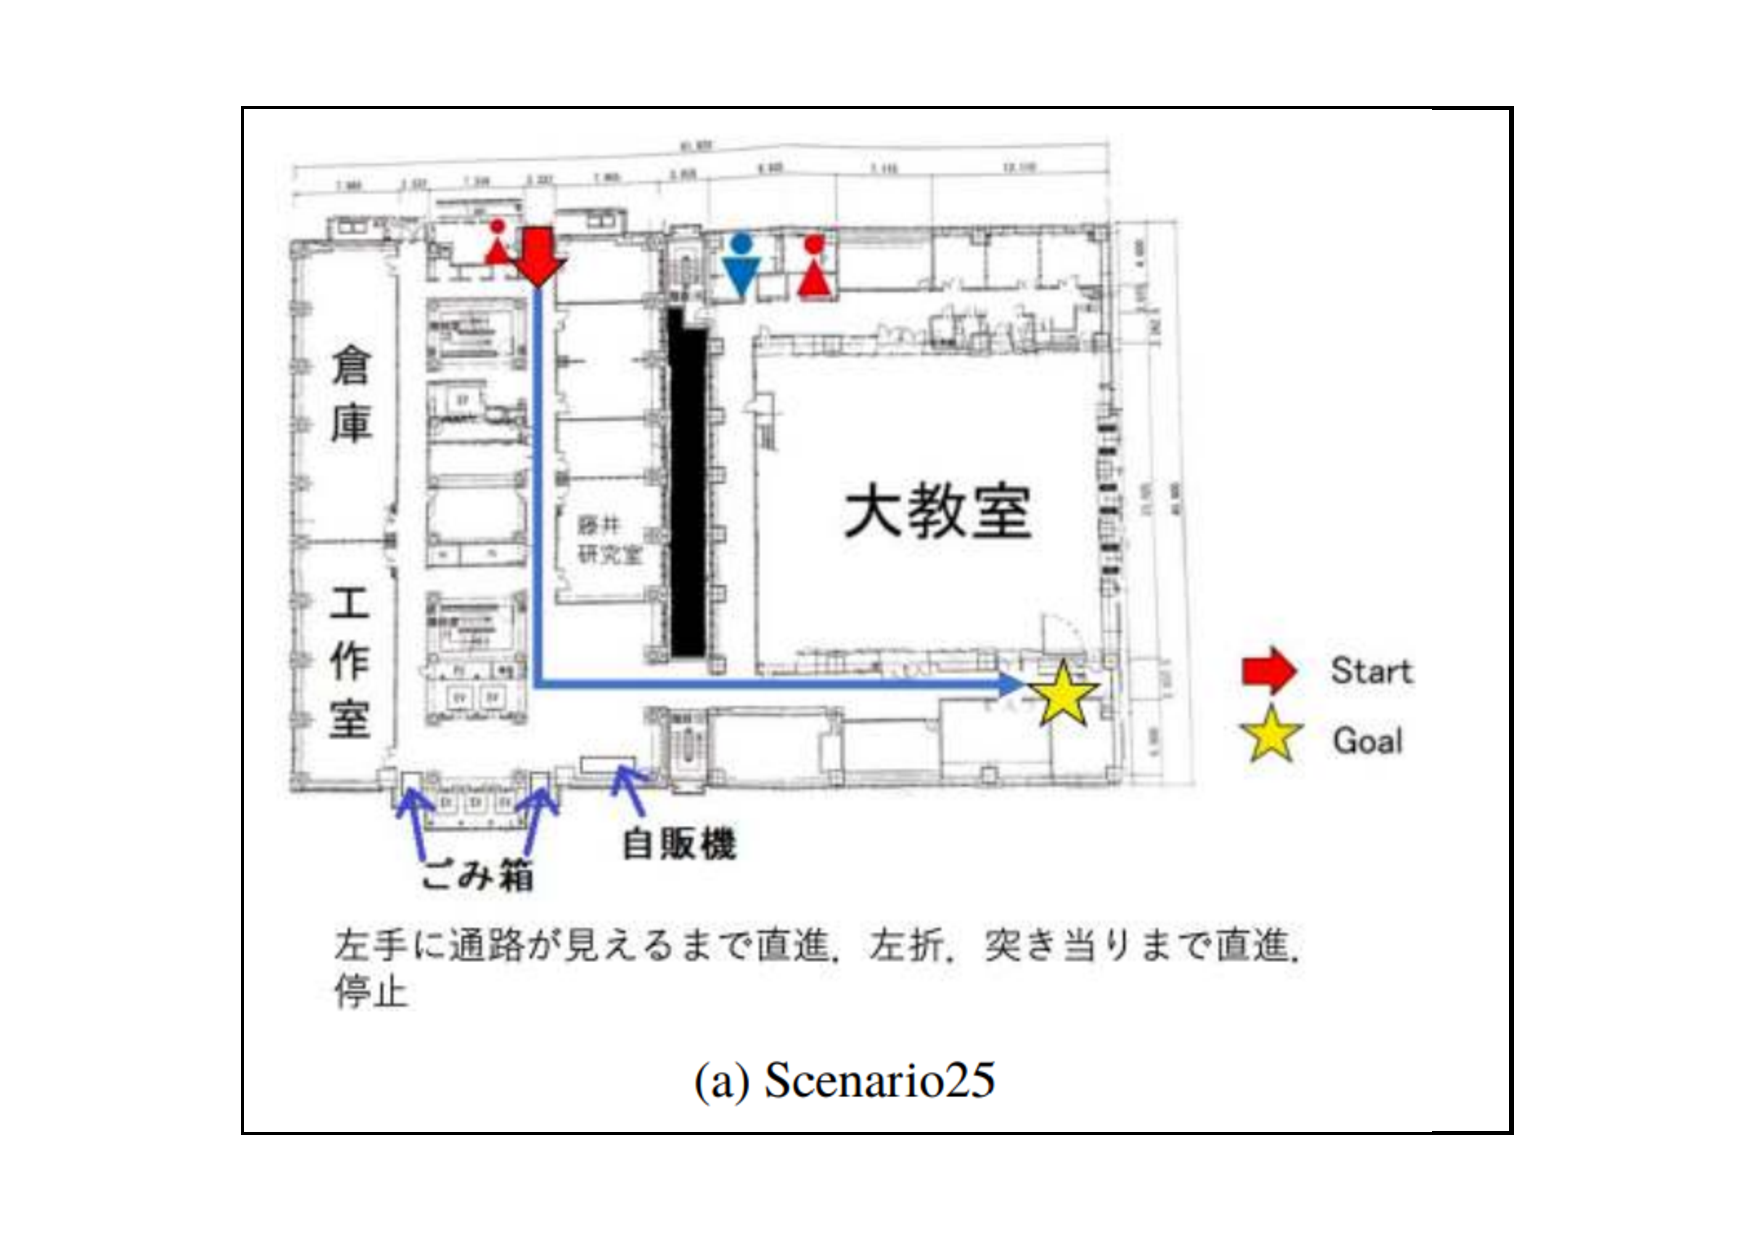
\includegraphics[keepaspectratio, width=80mm]{images/pdf/ishiguro/scenario/25.pdf}
        \subcaption{scenario25}
      \end{minipage} &
      \begin{minipage}[t]{0.48\textwidth}
        \centering
        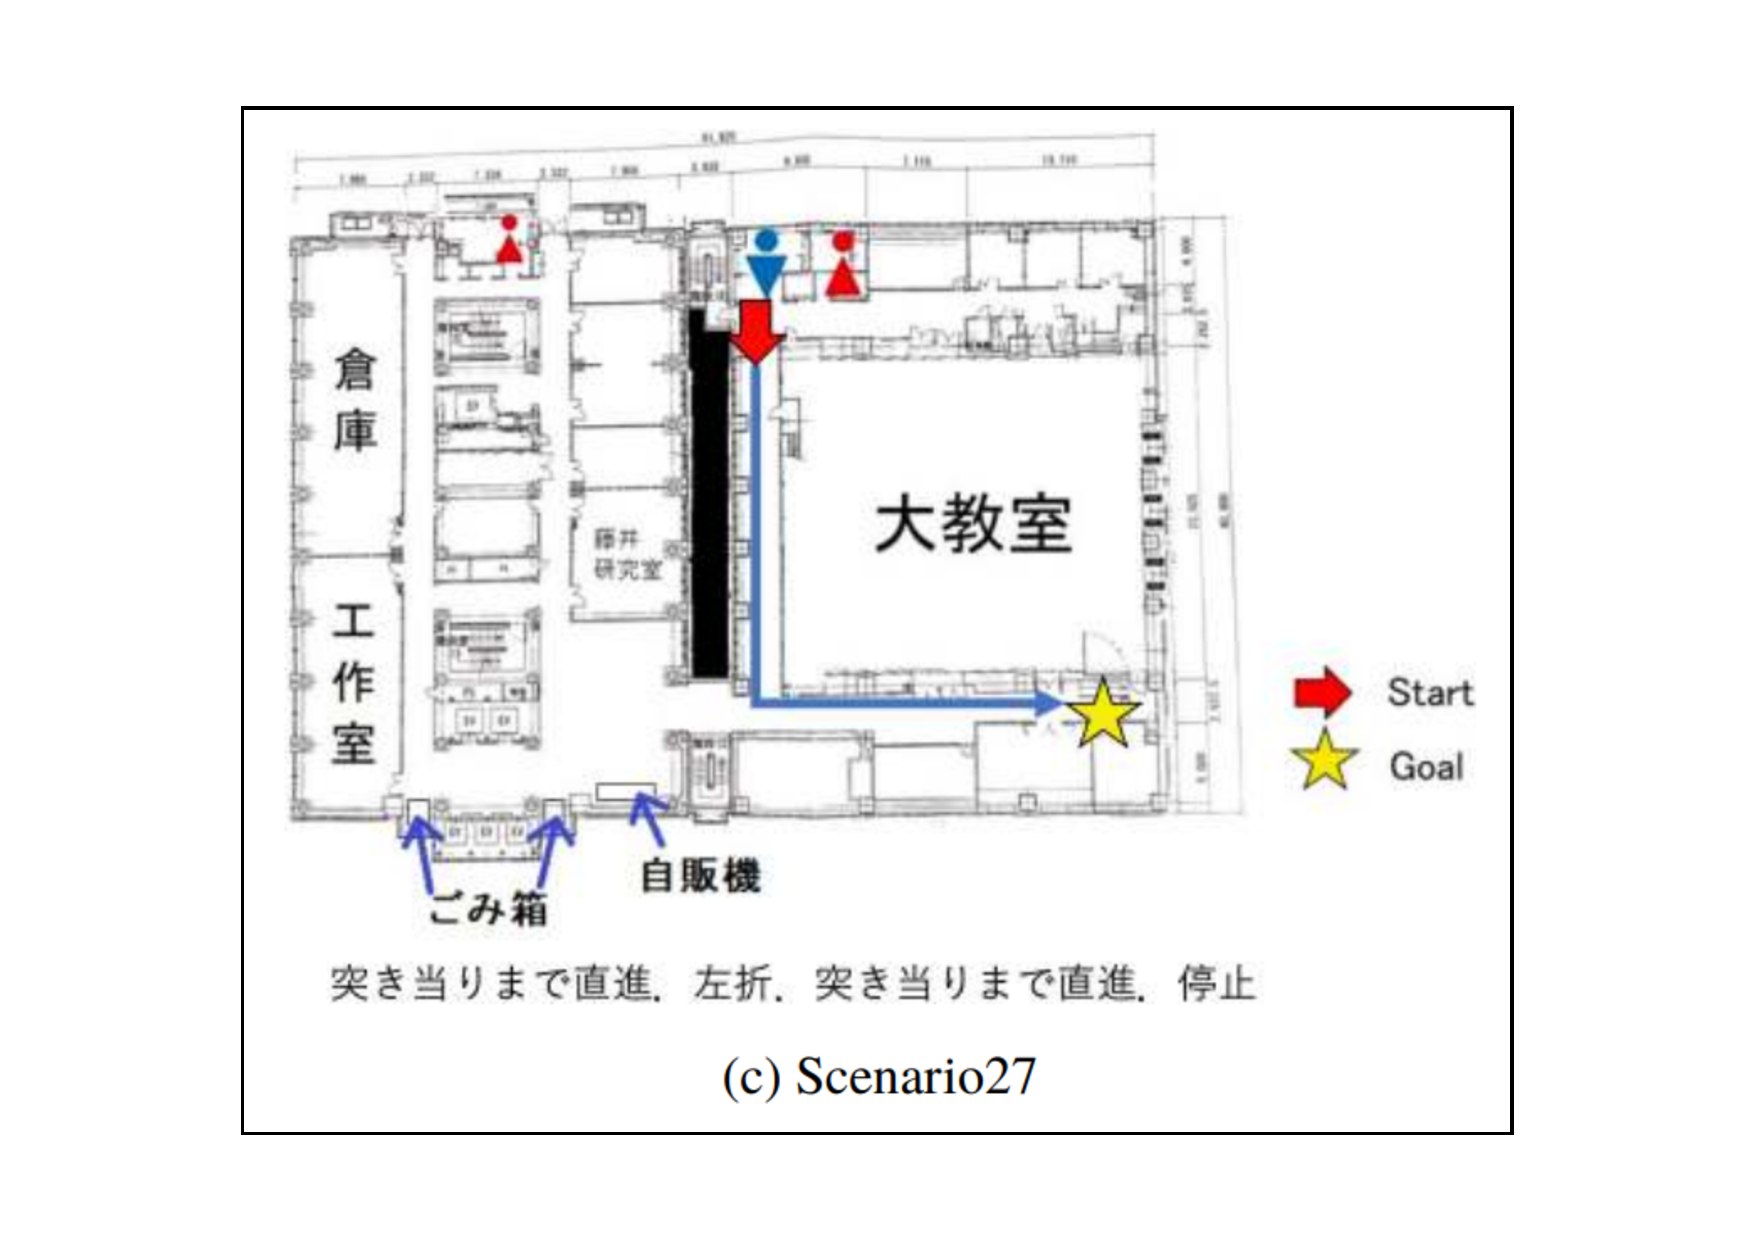
\includegraphics[keepaspectratio, width=80mm]{images/pdf/ishiguro/scenario/27.pdf}
        \subcaption{scenario27}
      \end{minipage}
  \end{tabular}
\caption{Scenarios 20 to 27}
\label{fig:scenario_20_27}
\end{figure*}

\begin{figure*}[htbp]
  \begin{tabular}{cc}
      \begin{minipage}[t]{0.48\textwidth}
        \centering
        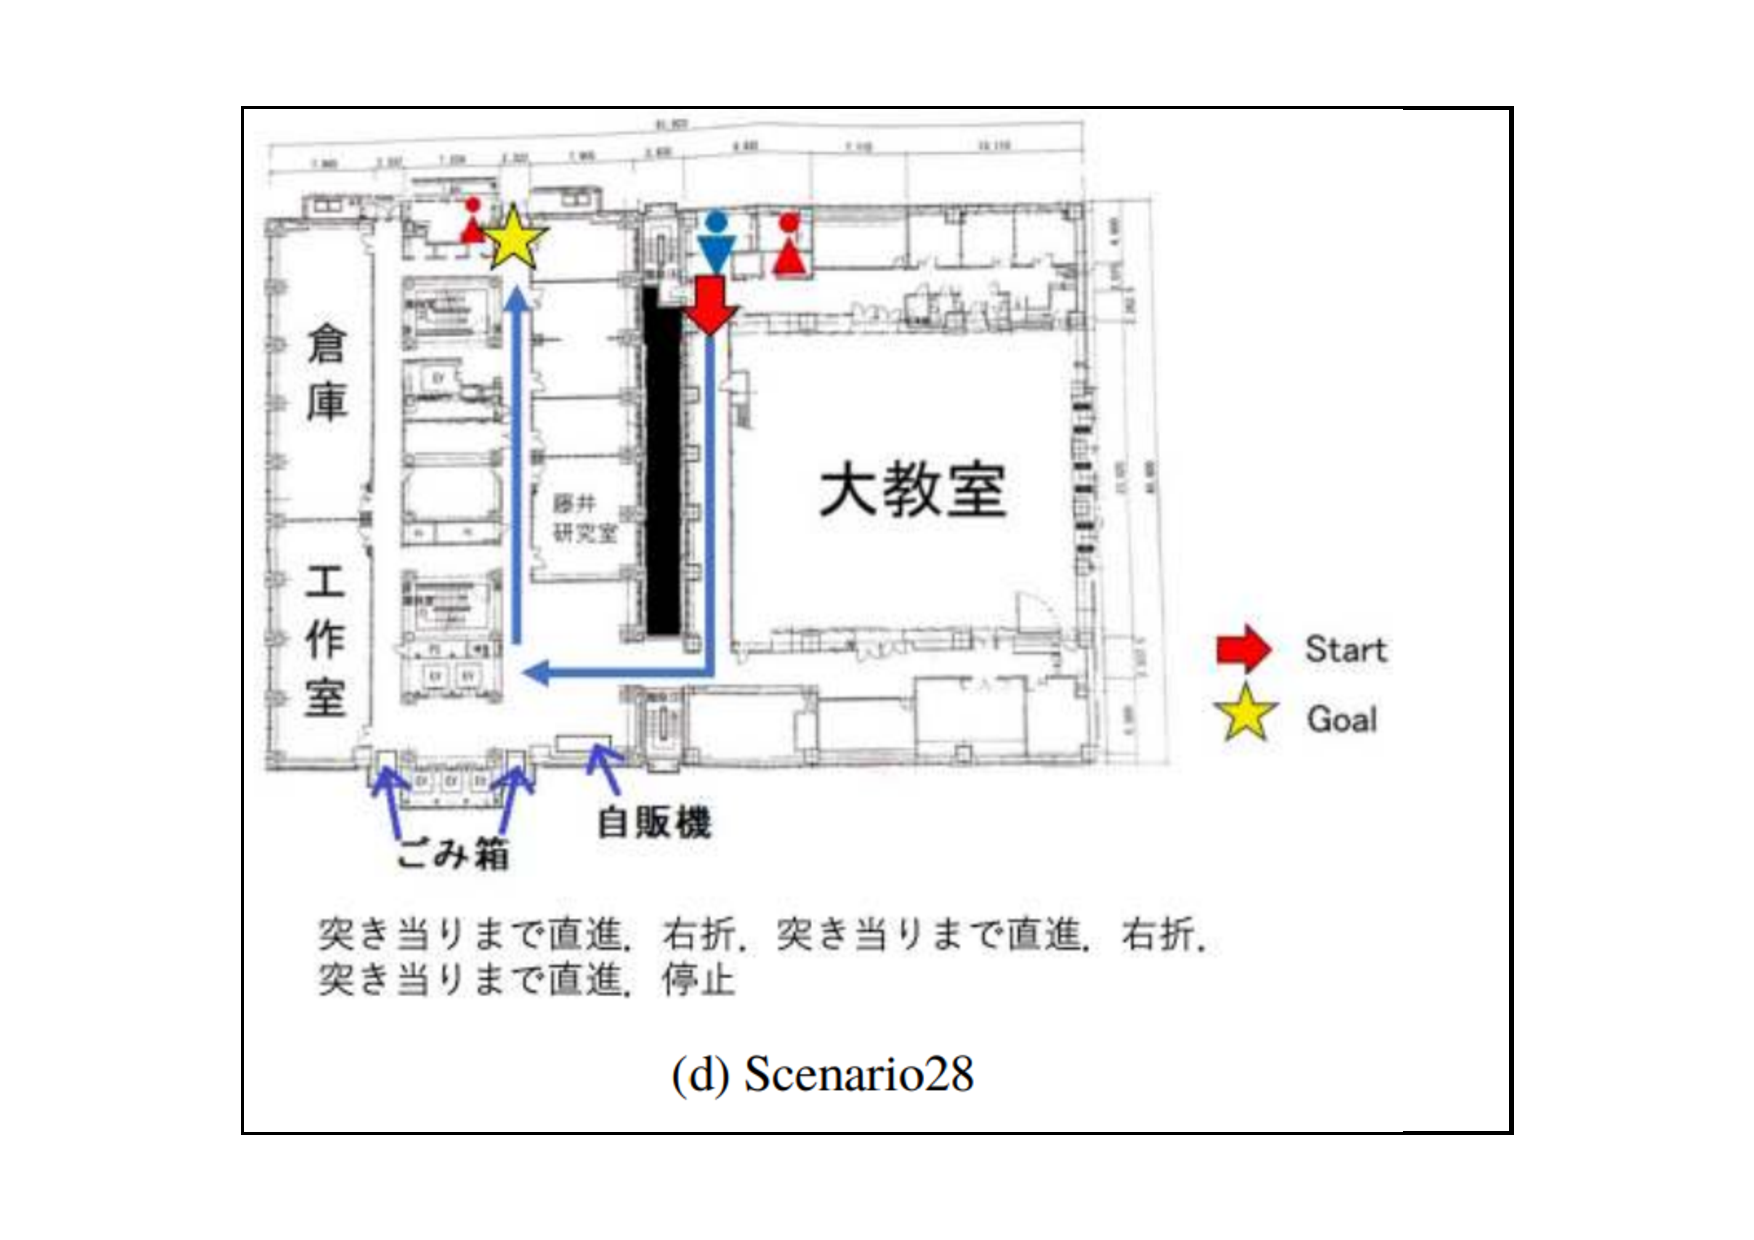
\includegraphics[keepaspectratio, width=80mm]{images/pdf/ishiguro/scenario/28.pdf}
        \subcaption{scenario28}
      \end{minipage} &
      \begin{minipage}[t]{0.48\textwidth}
        \centering
        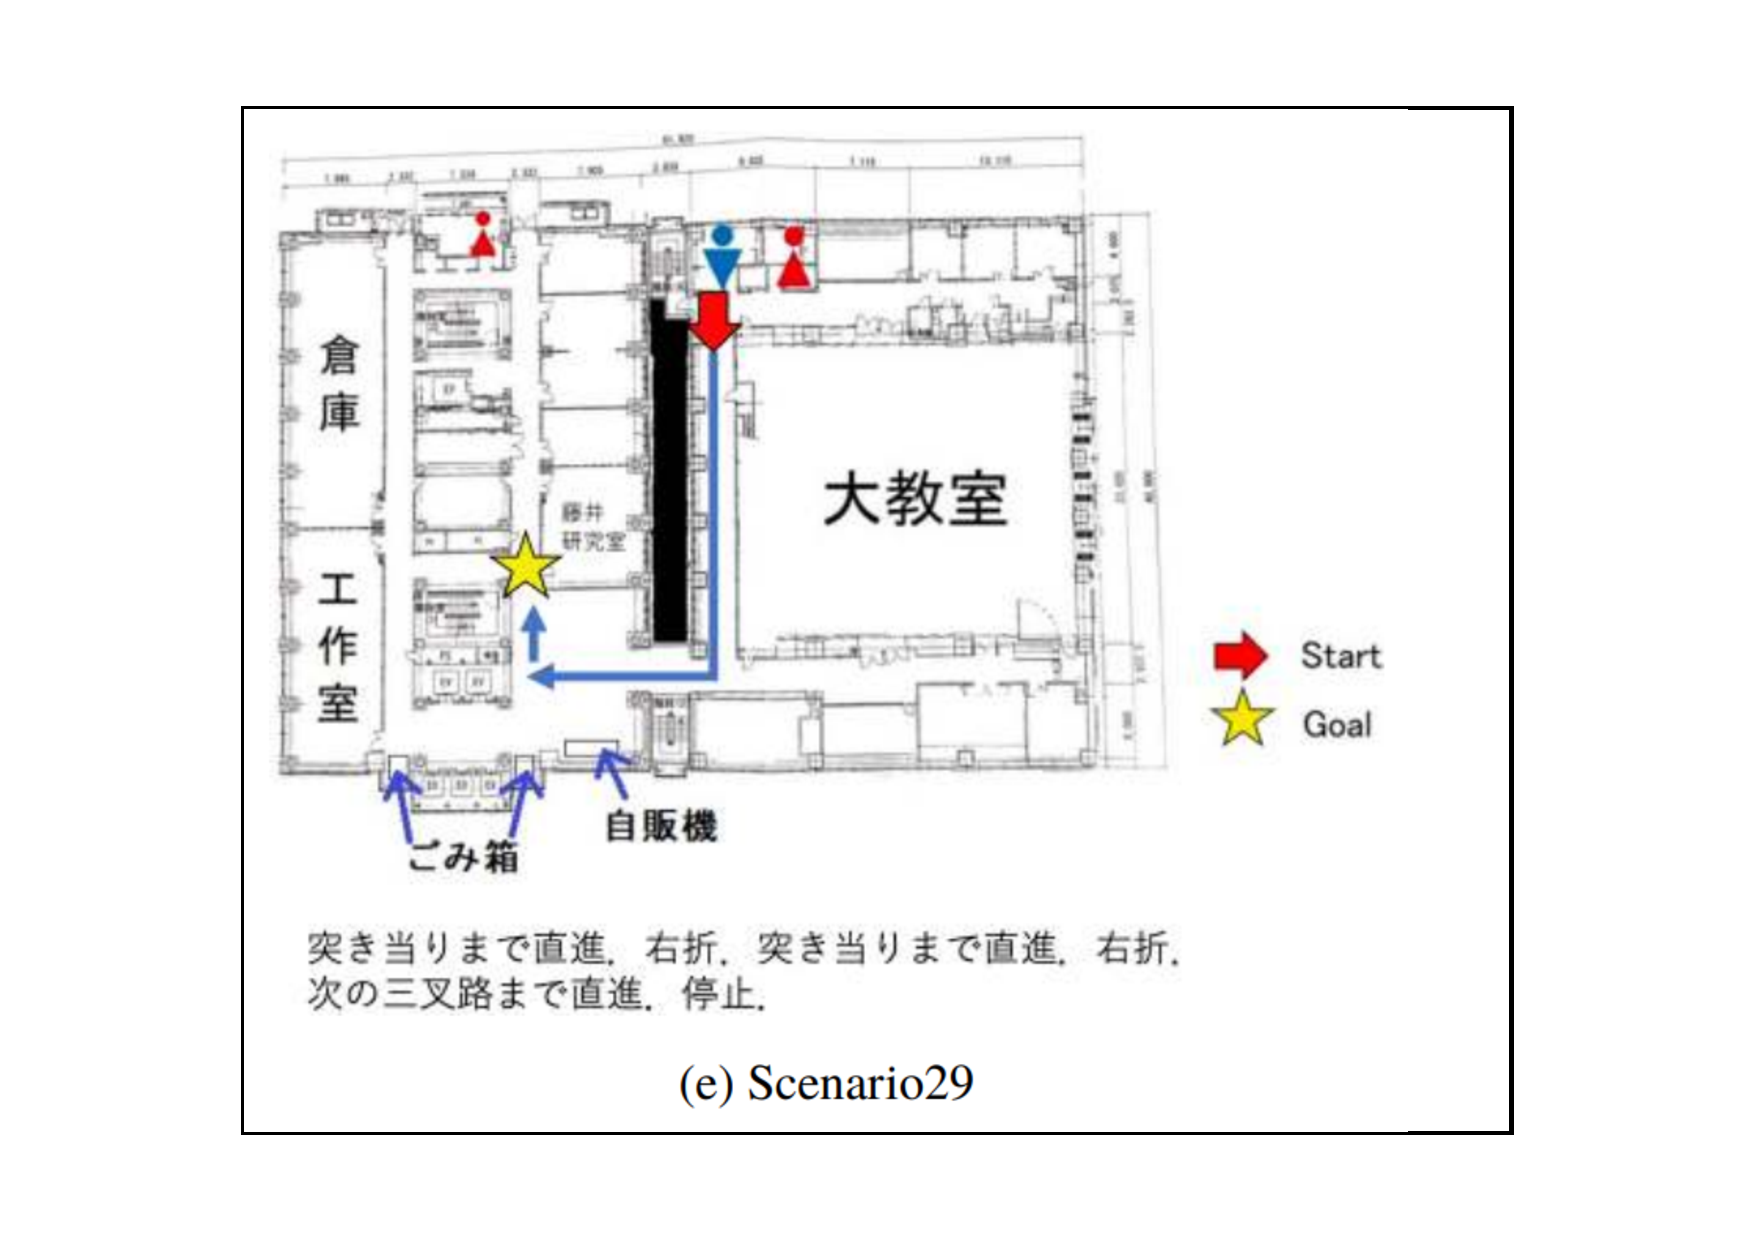
\includegraphics[keepaspectratio, width=80mm]{images/pdf/ishiguro/scenario/29.pdf}
        \subcaption{scenario29}
      \end{minipage} \\
      \begin{minipage}[t]{0.48\textwidth}
        \centering
        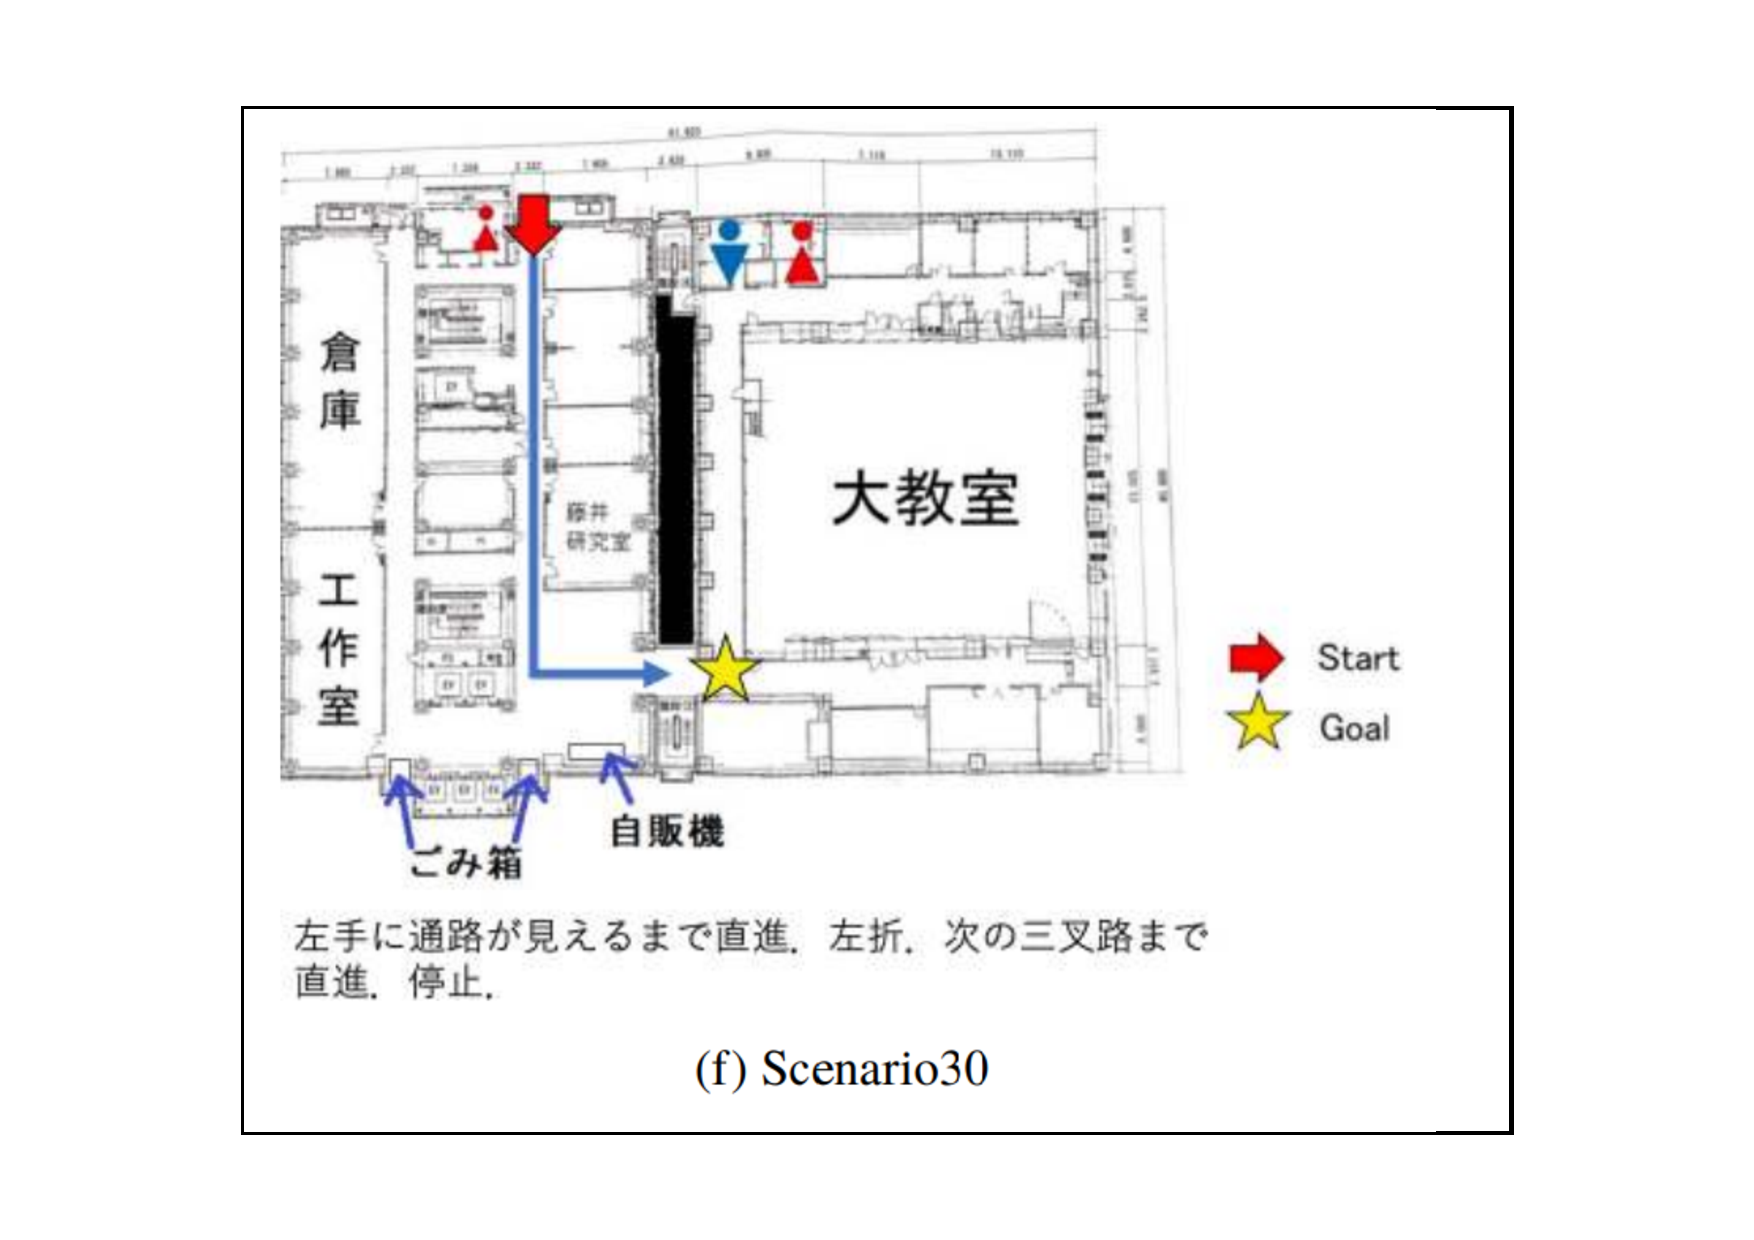
\includegraphics[keepaspectratio, width=80mm]{images/pdf/ishiguro/scenario/30.pdf}
        \subcaption{scenario30}
      \end{minipage} &
      \begin{minipage}[t]{0.48\textwidth}
        \centering
        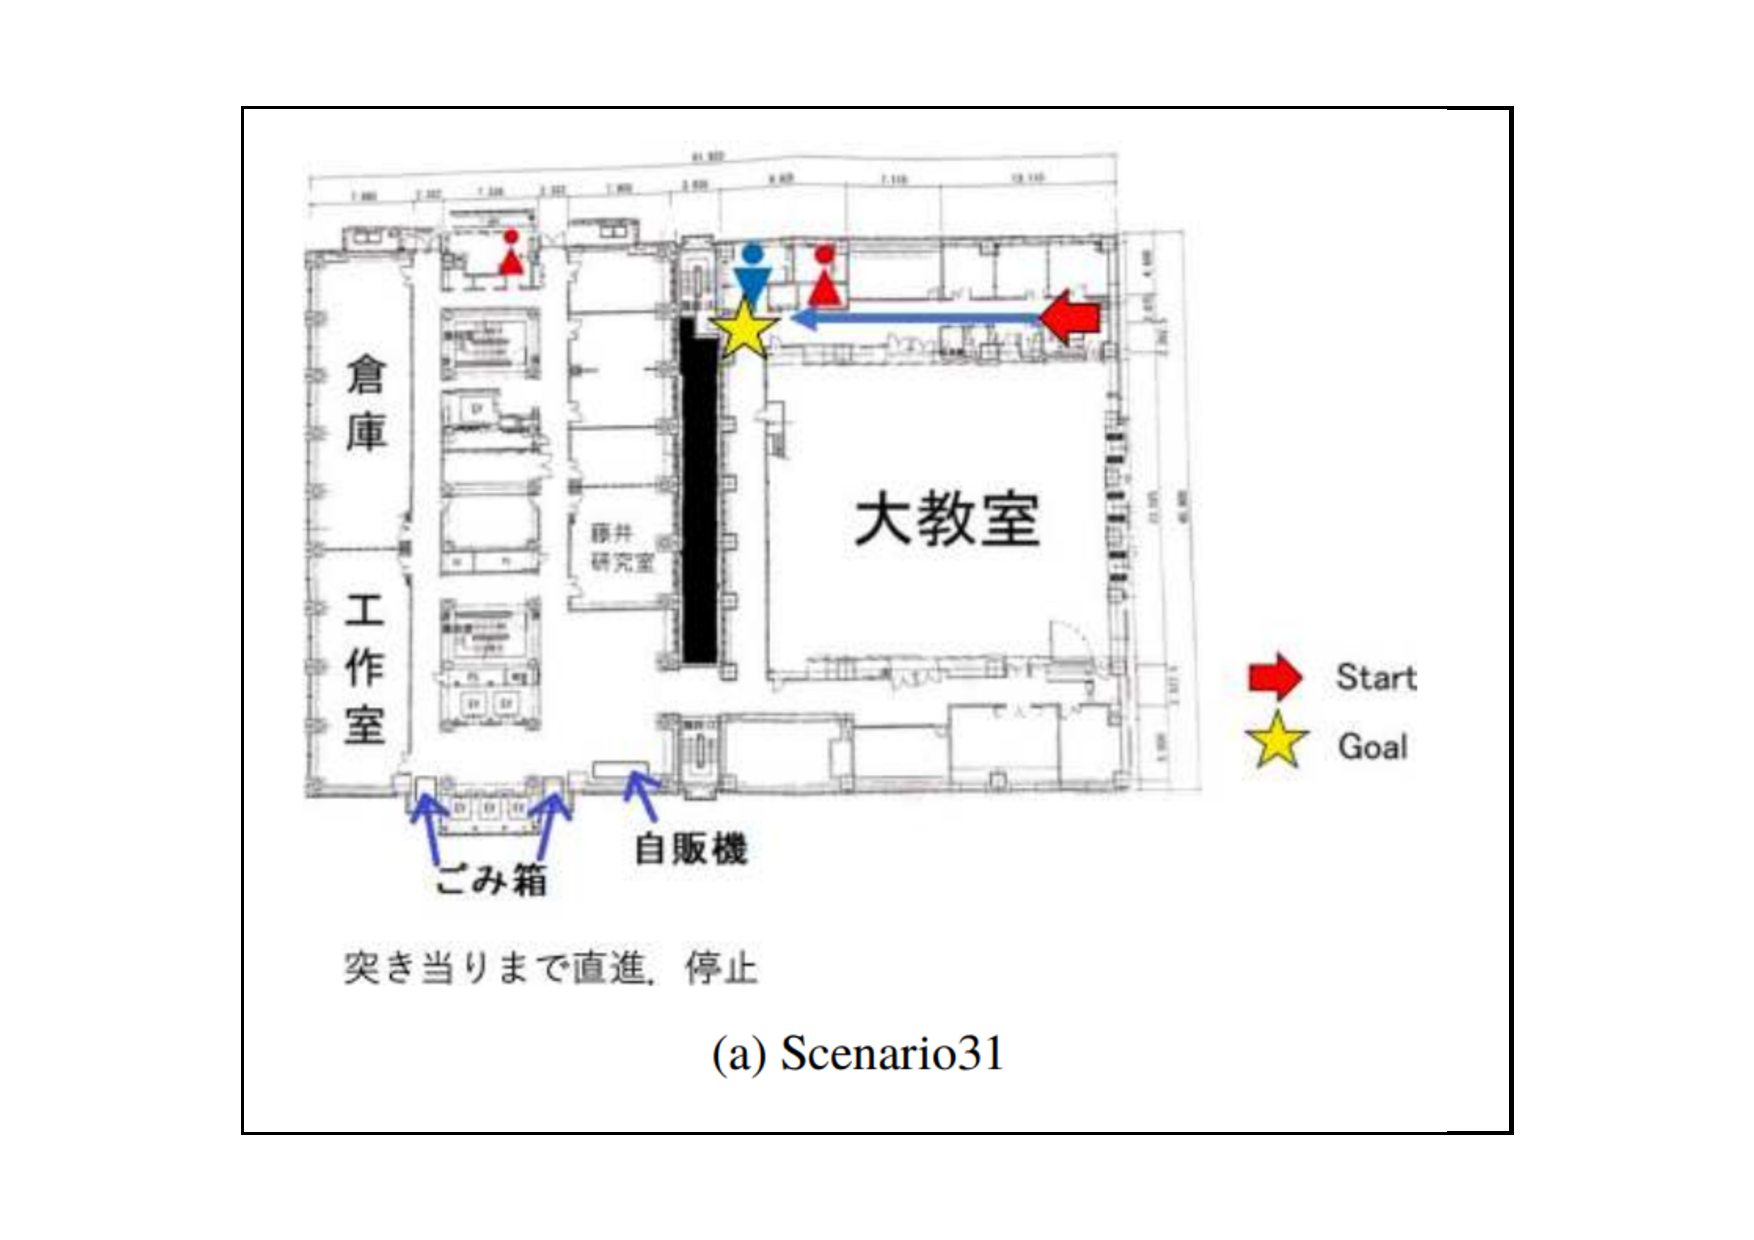
\includegraphics[keepaspectratio, width=80mm]{images/pdf/ishiguro/scenario/31.pdf}
        \subcaption{scenario31}
      \end{minipage} \\
      \begin{minipage}[t]{0.48\textwidth}
        \centering
        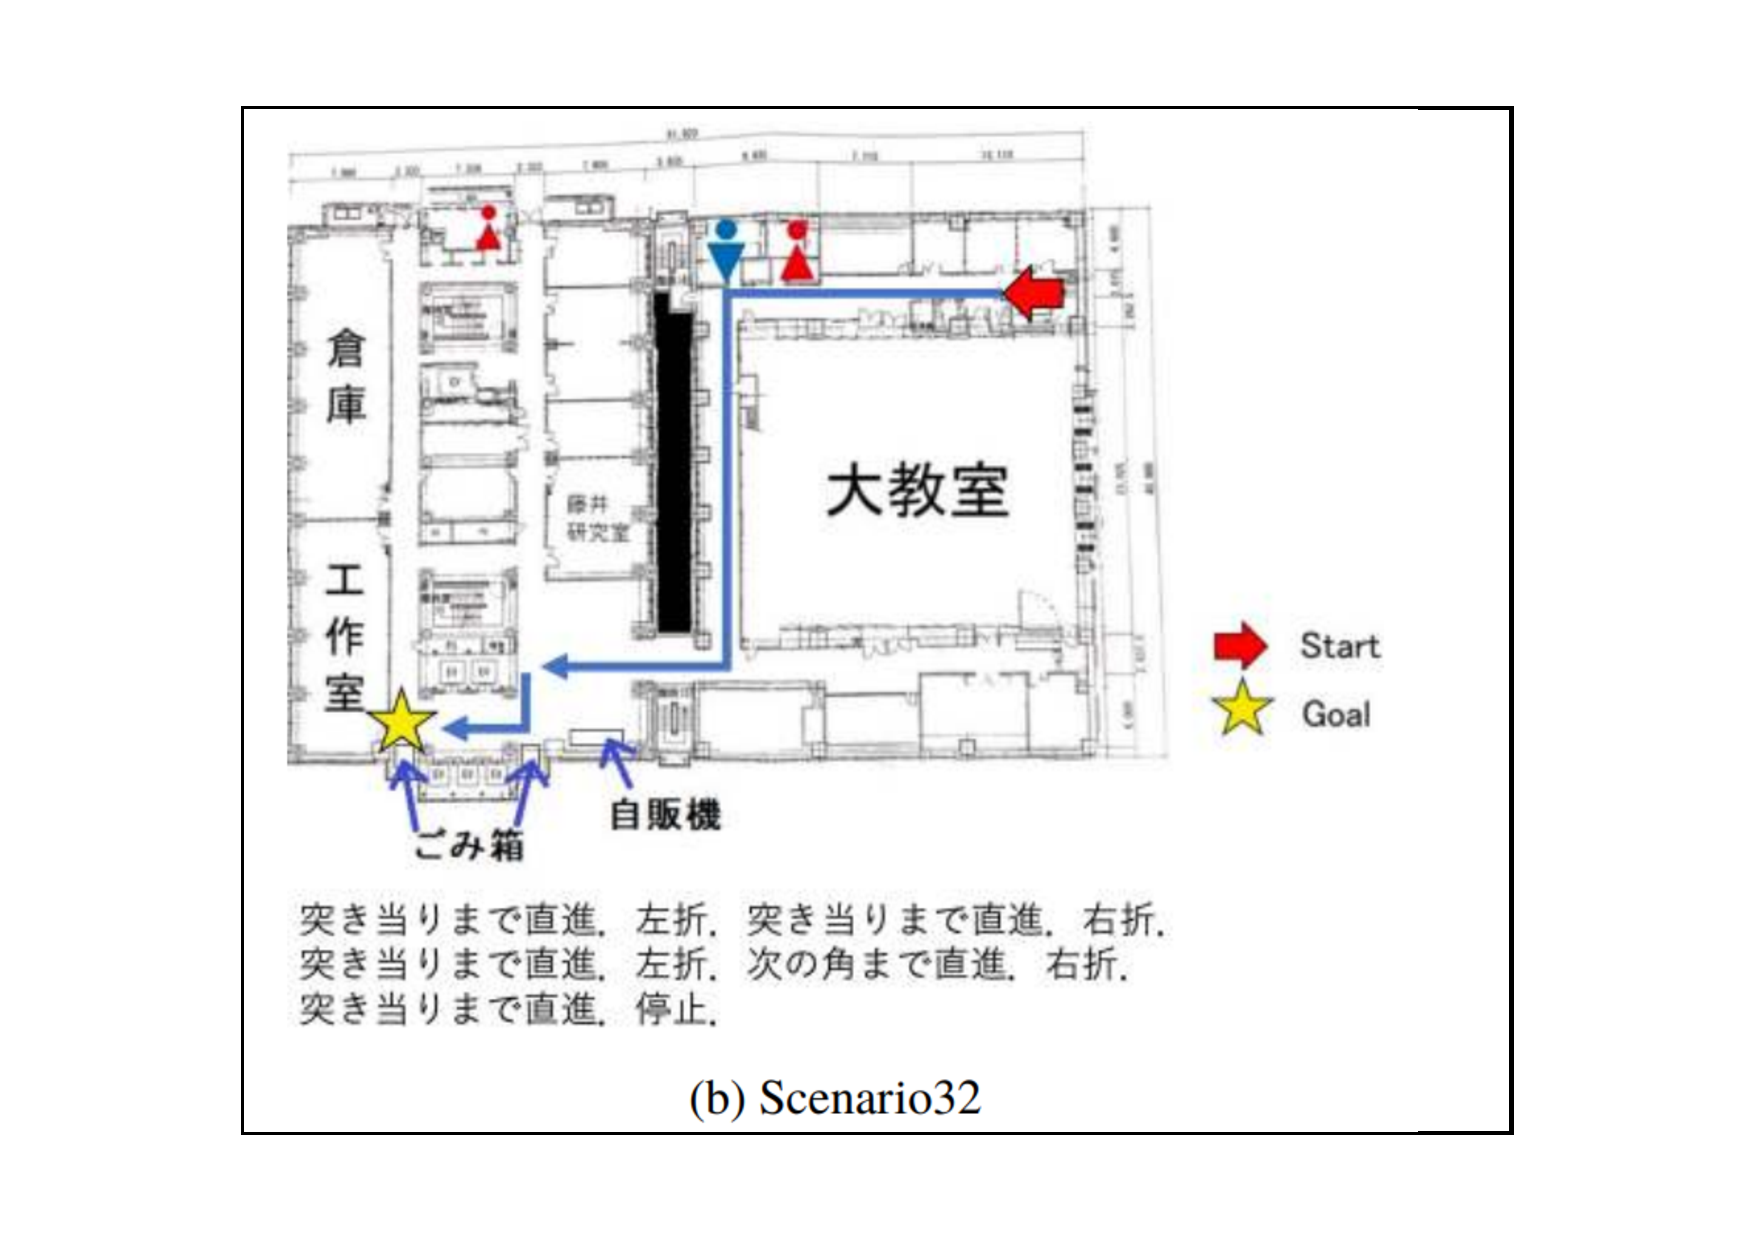
\includegraphics[keepaspectratio, width=80mm]{images/pdf/ishiguro/scenario/32.pdf}
        \subcaption{scenario32}
      \end{minipage} &
      \begin{minipage}[t]{0.48\textwidth}
        \centering
        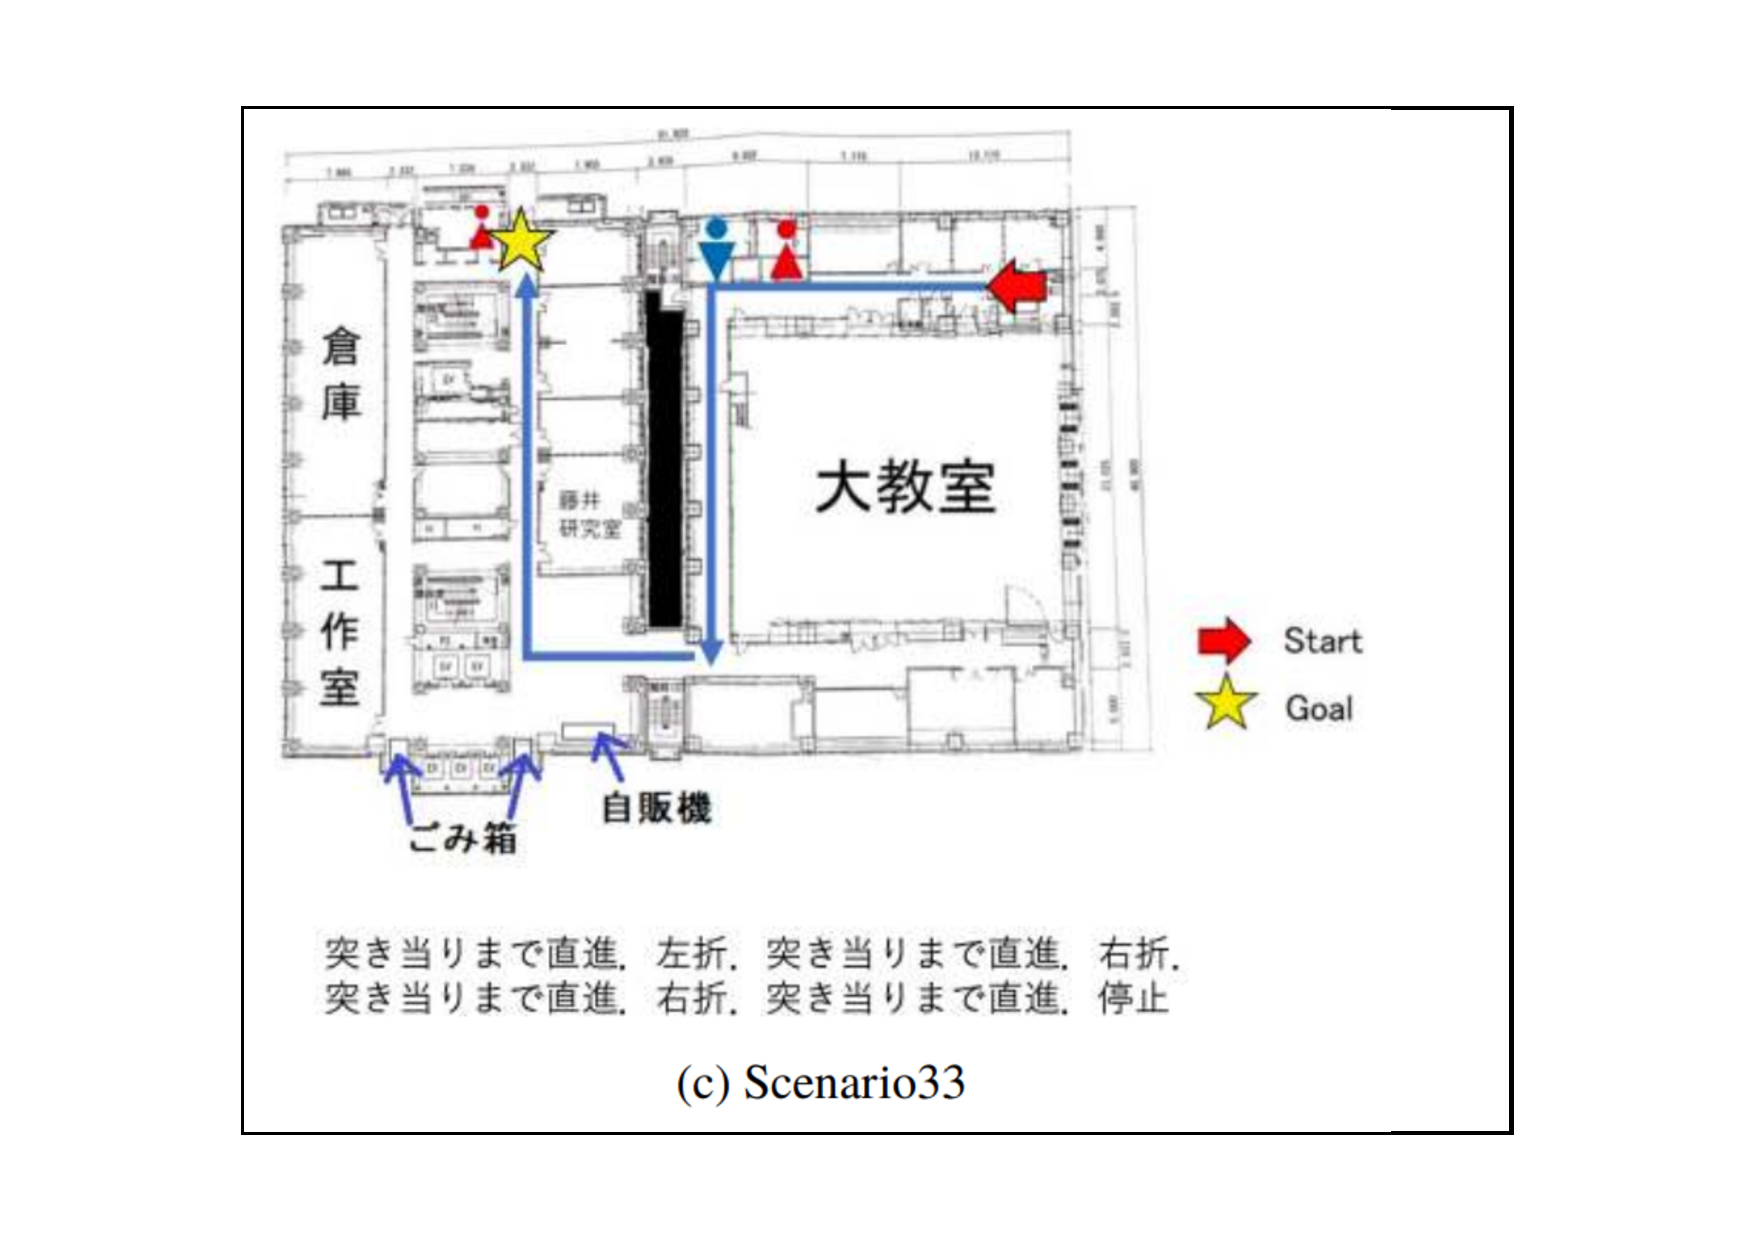
\includegraphics[keepaspectratio, width=80mm]{images/pdf/ishiguro/scenario/33.pdf}
        \subcaption{scenario33}
      \end{minipage}
  \end{tabular}
\caption{Scenarios 28 to 33}
\label{fig:scenario_28_33}
\end{figure*}

\begin{figure*}[htbp]
  \begin{tabular}{cc}
      \begin{minipage}[t]{0.48\textwidth}
        \centering
        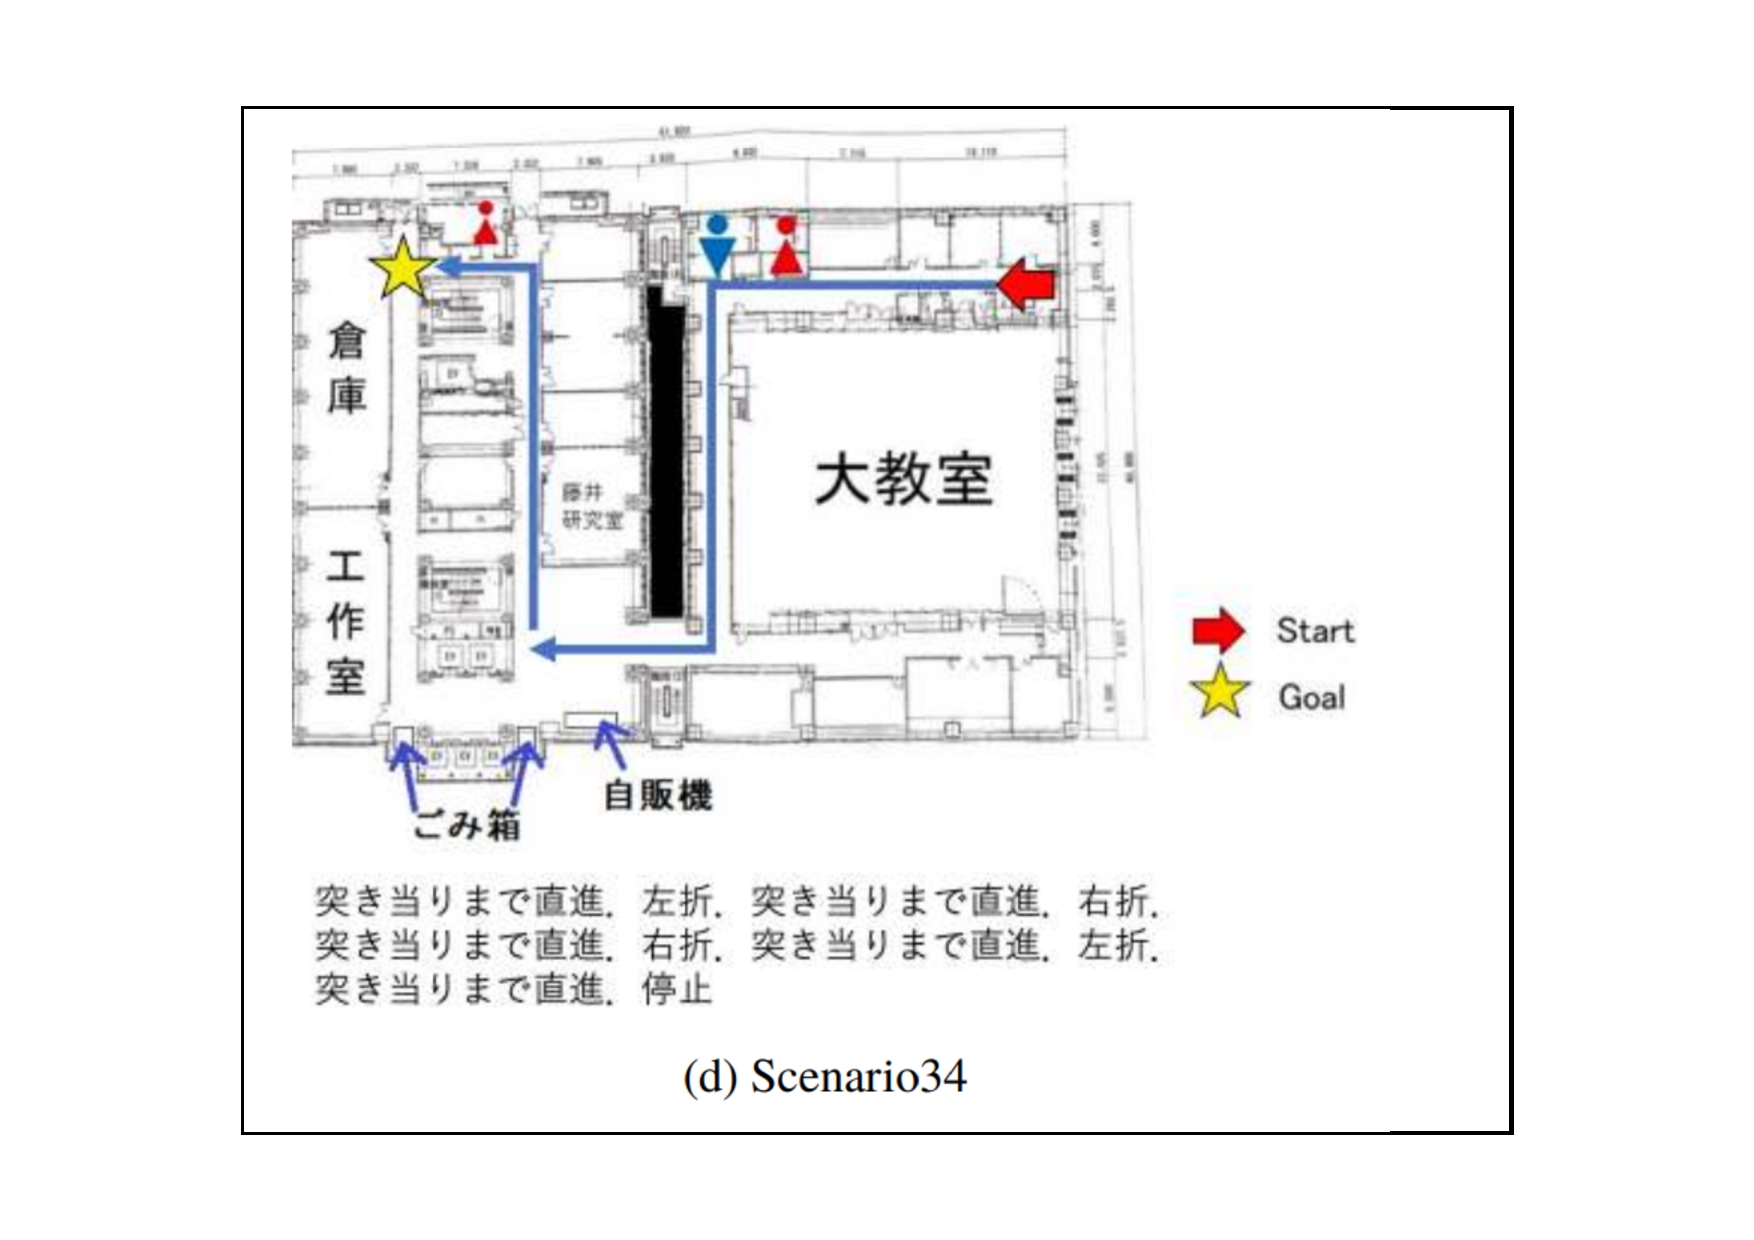
\includegraphics[keepaspectratio, width=80mm]{images/pdf/ishiguro/scenario/34.pdf}
        \subcaption{scenario34}
      \end{minipage} &
      \begin{minipage}[t]{0.48\textwidth}
        \centering
        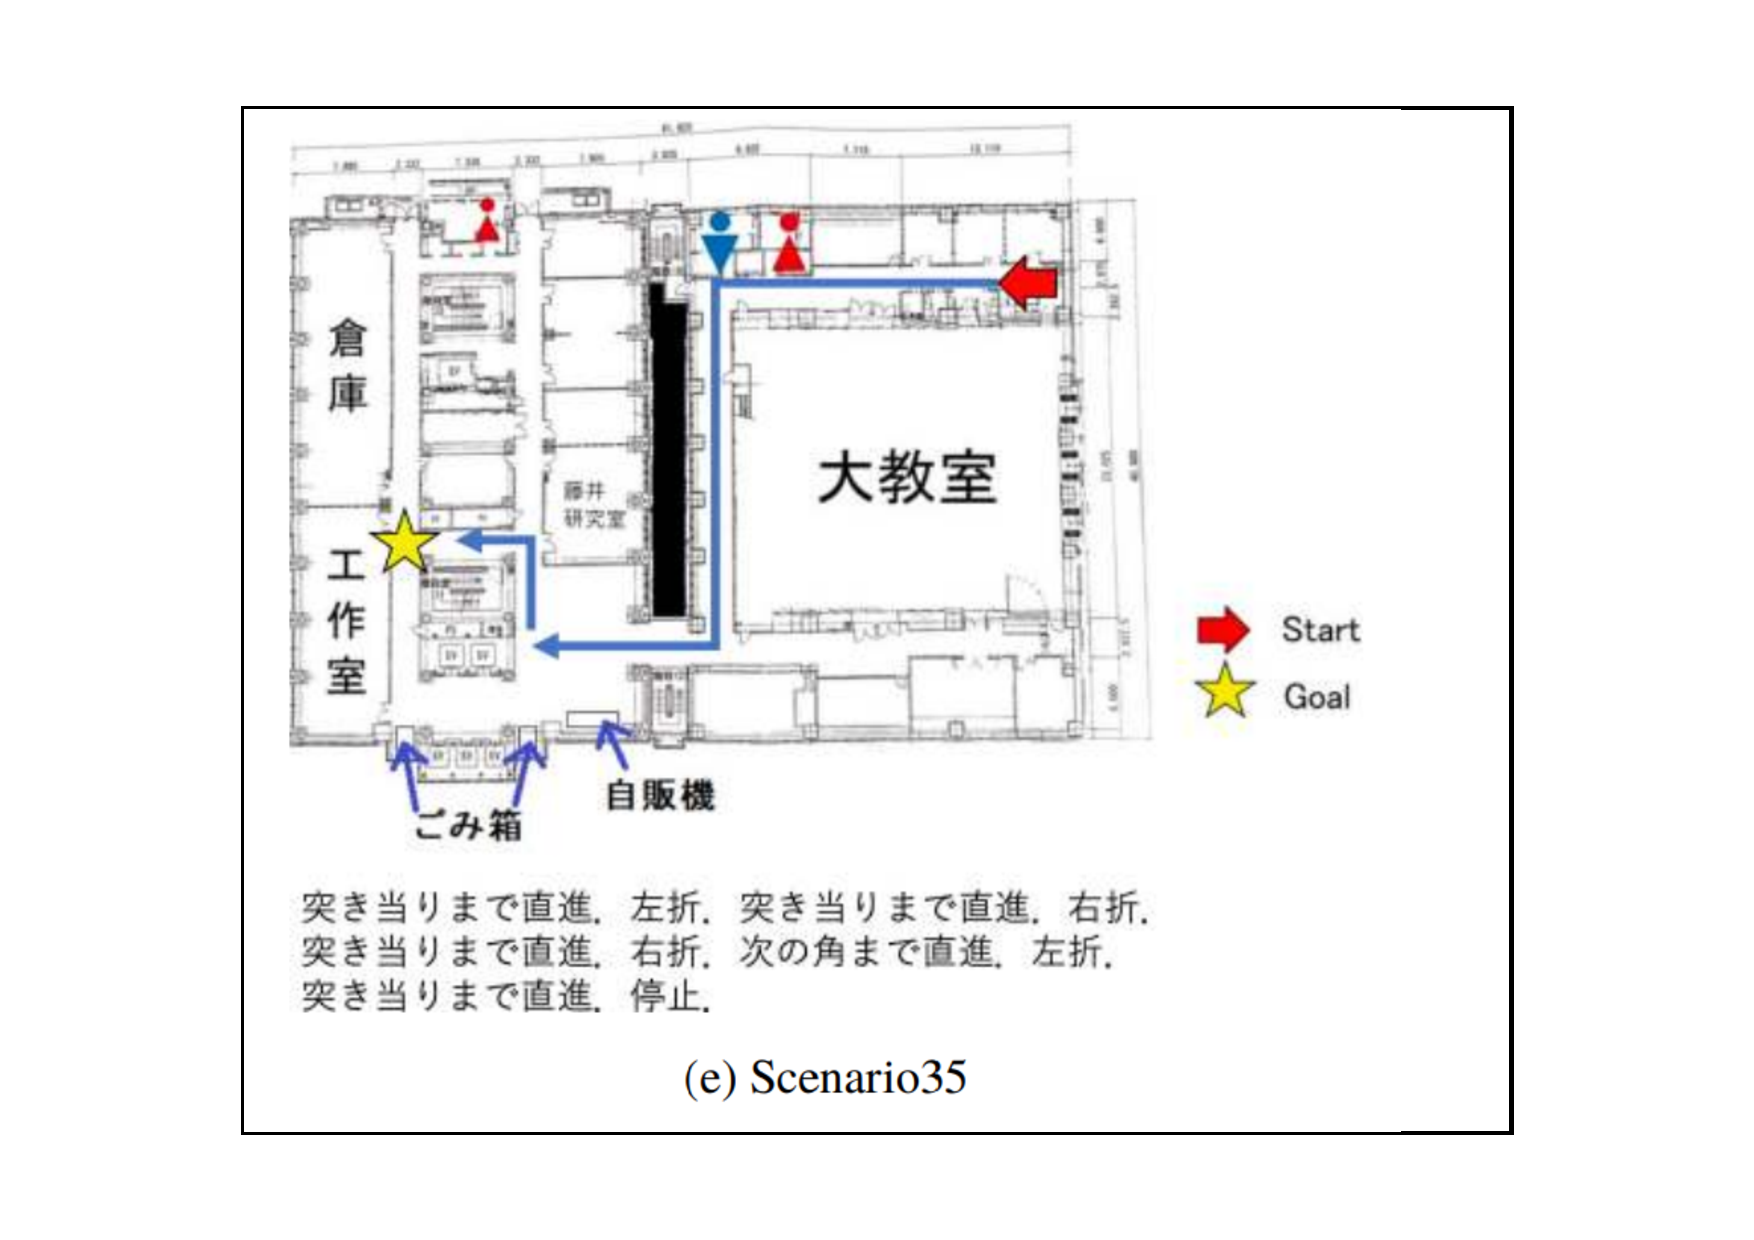
\includegraphics[keepaspectratio, width=80mm]{images/pdf/ishiguro/scenario/35.pdf}
        \subcaption{scenario35}
      \end{minipage} \\
      \begin{minipage}[t]{0.48\textwidth}
        \centering
        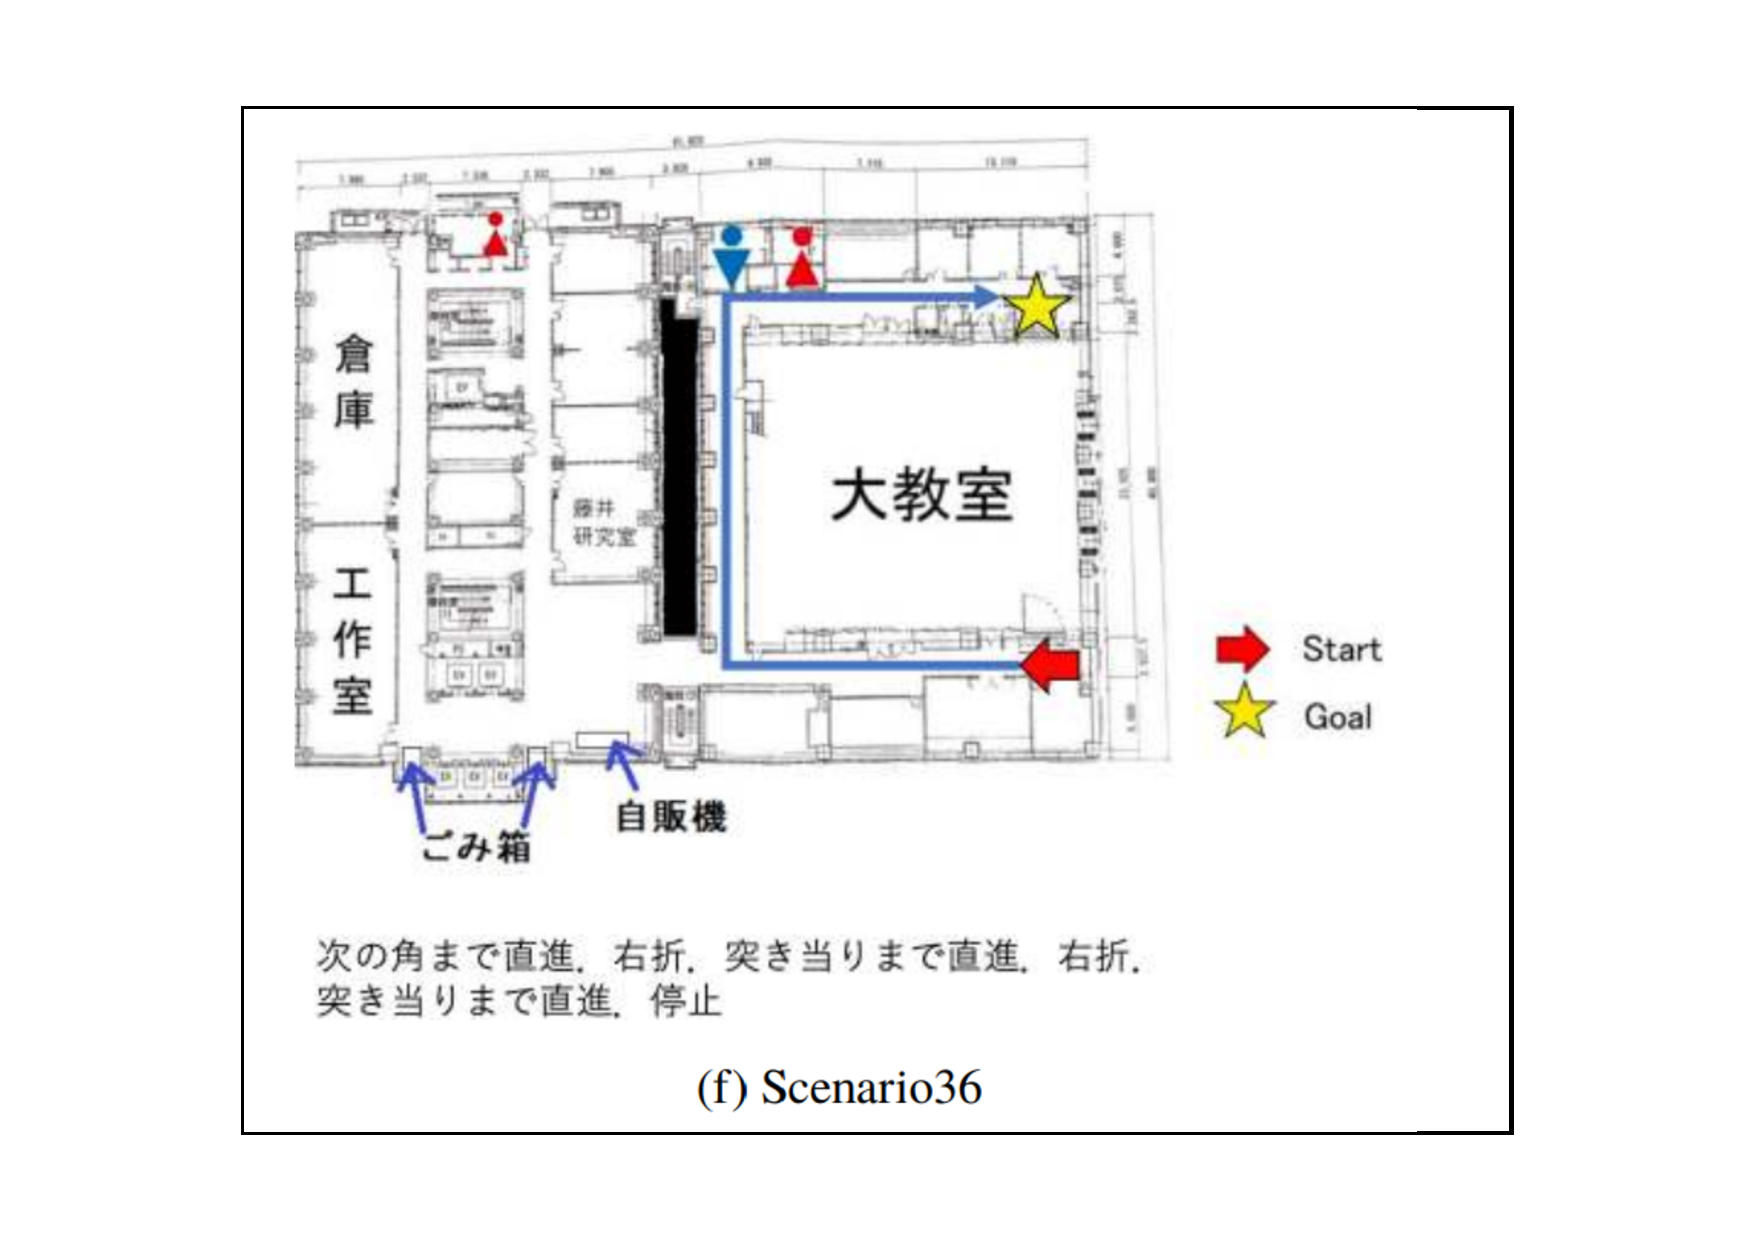
\includegraphics[keepaspectratio, width=80mm]{images/pdf/ishiguro/scenario/36.pdf}
        \subcaption{scenario36}
      \end{minipage} &
      \begin{minipage}[t]{0.48\textwidth}
        \centering
        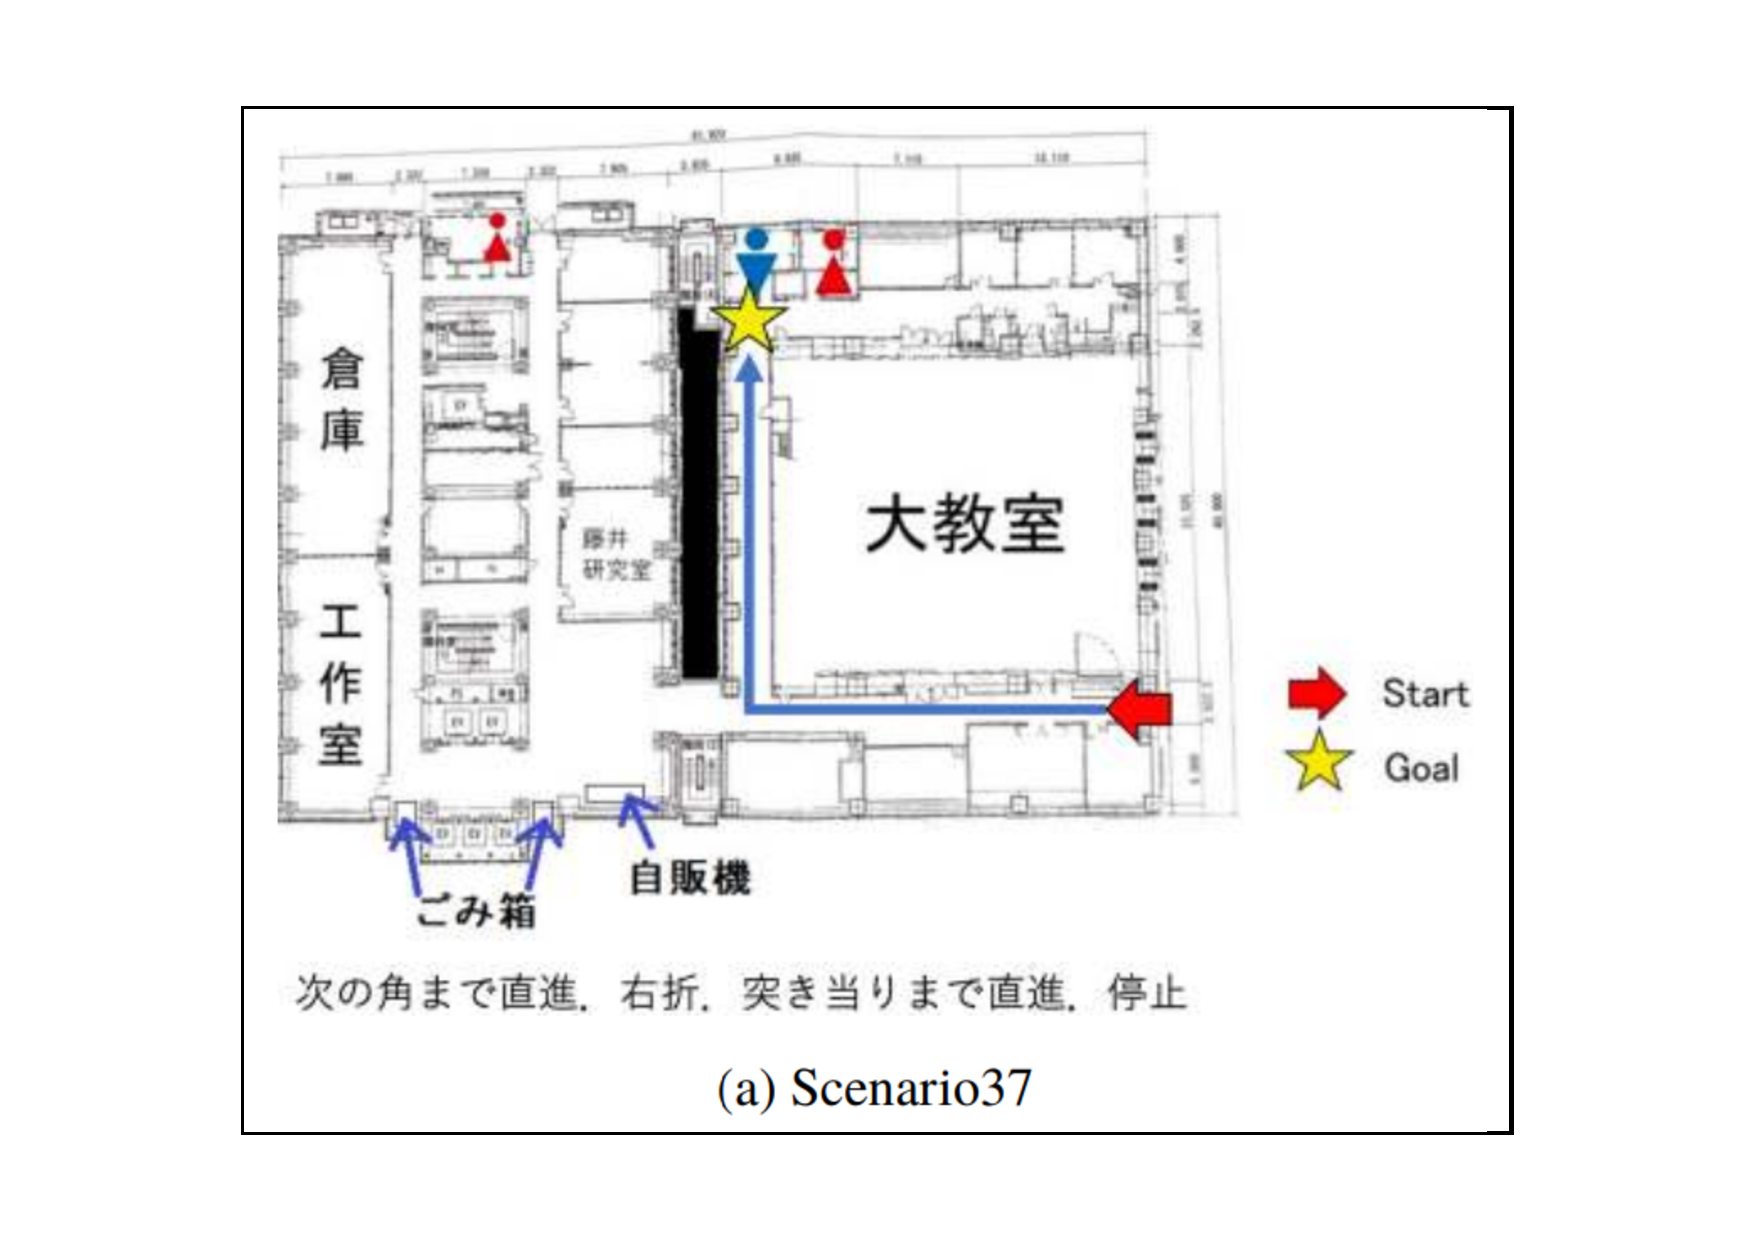
\includegraphics[keepaspectratio, width=80mm]{images/pdf/ishiguro/scenario/37.pdf}
        \subcaption{scenario37}
      \end{minipage} \\
      \begin{minipage}[t]{0.48\textwidth}
        \centering
        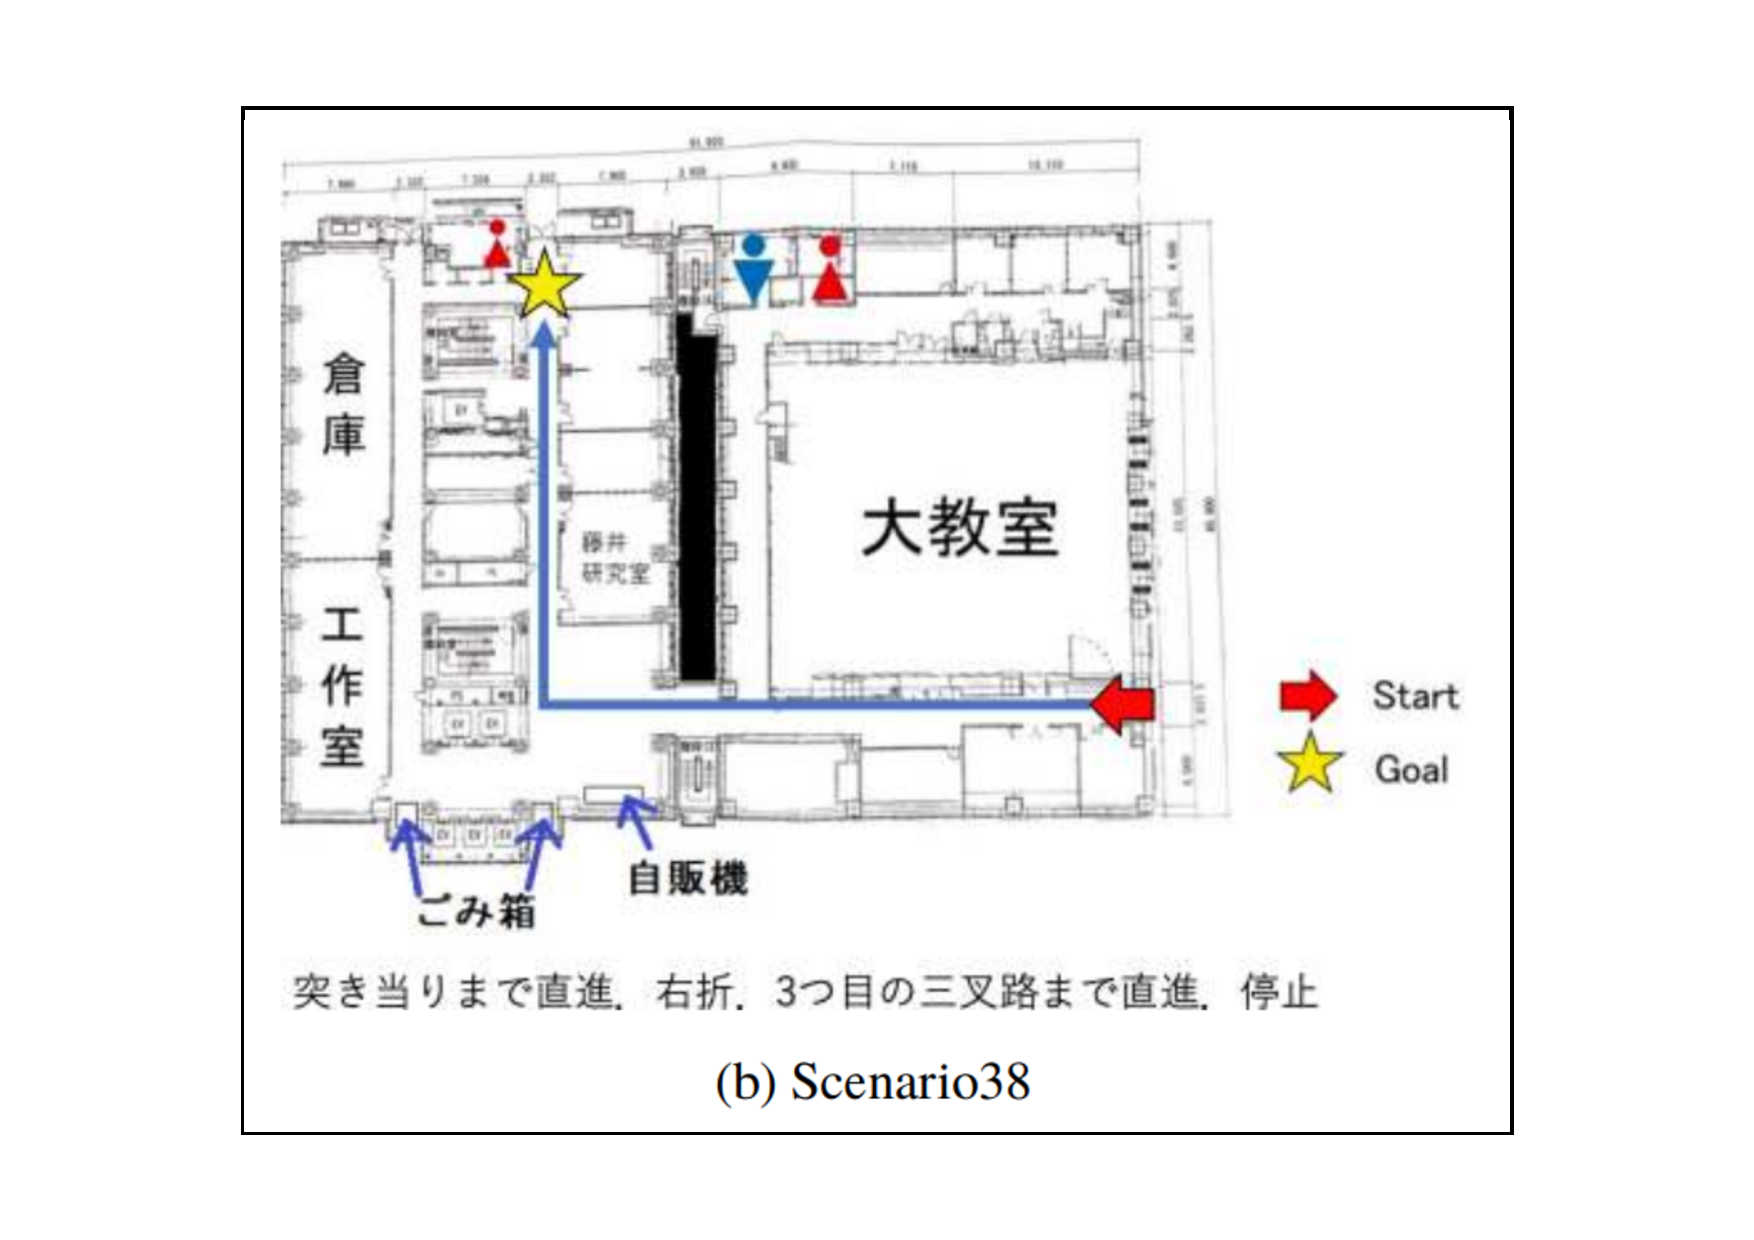
\includegraphics[keepaspectratio, width=80mm]{images/pdf/ishiguro/scenario/38.pdf}
        \subcaption{scenario38}
      \end{minipage} &
      \begin{minipage}[t]{0.48\textwidth}
        \centering
        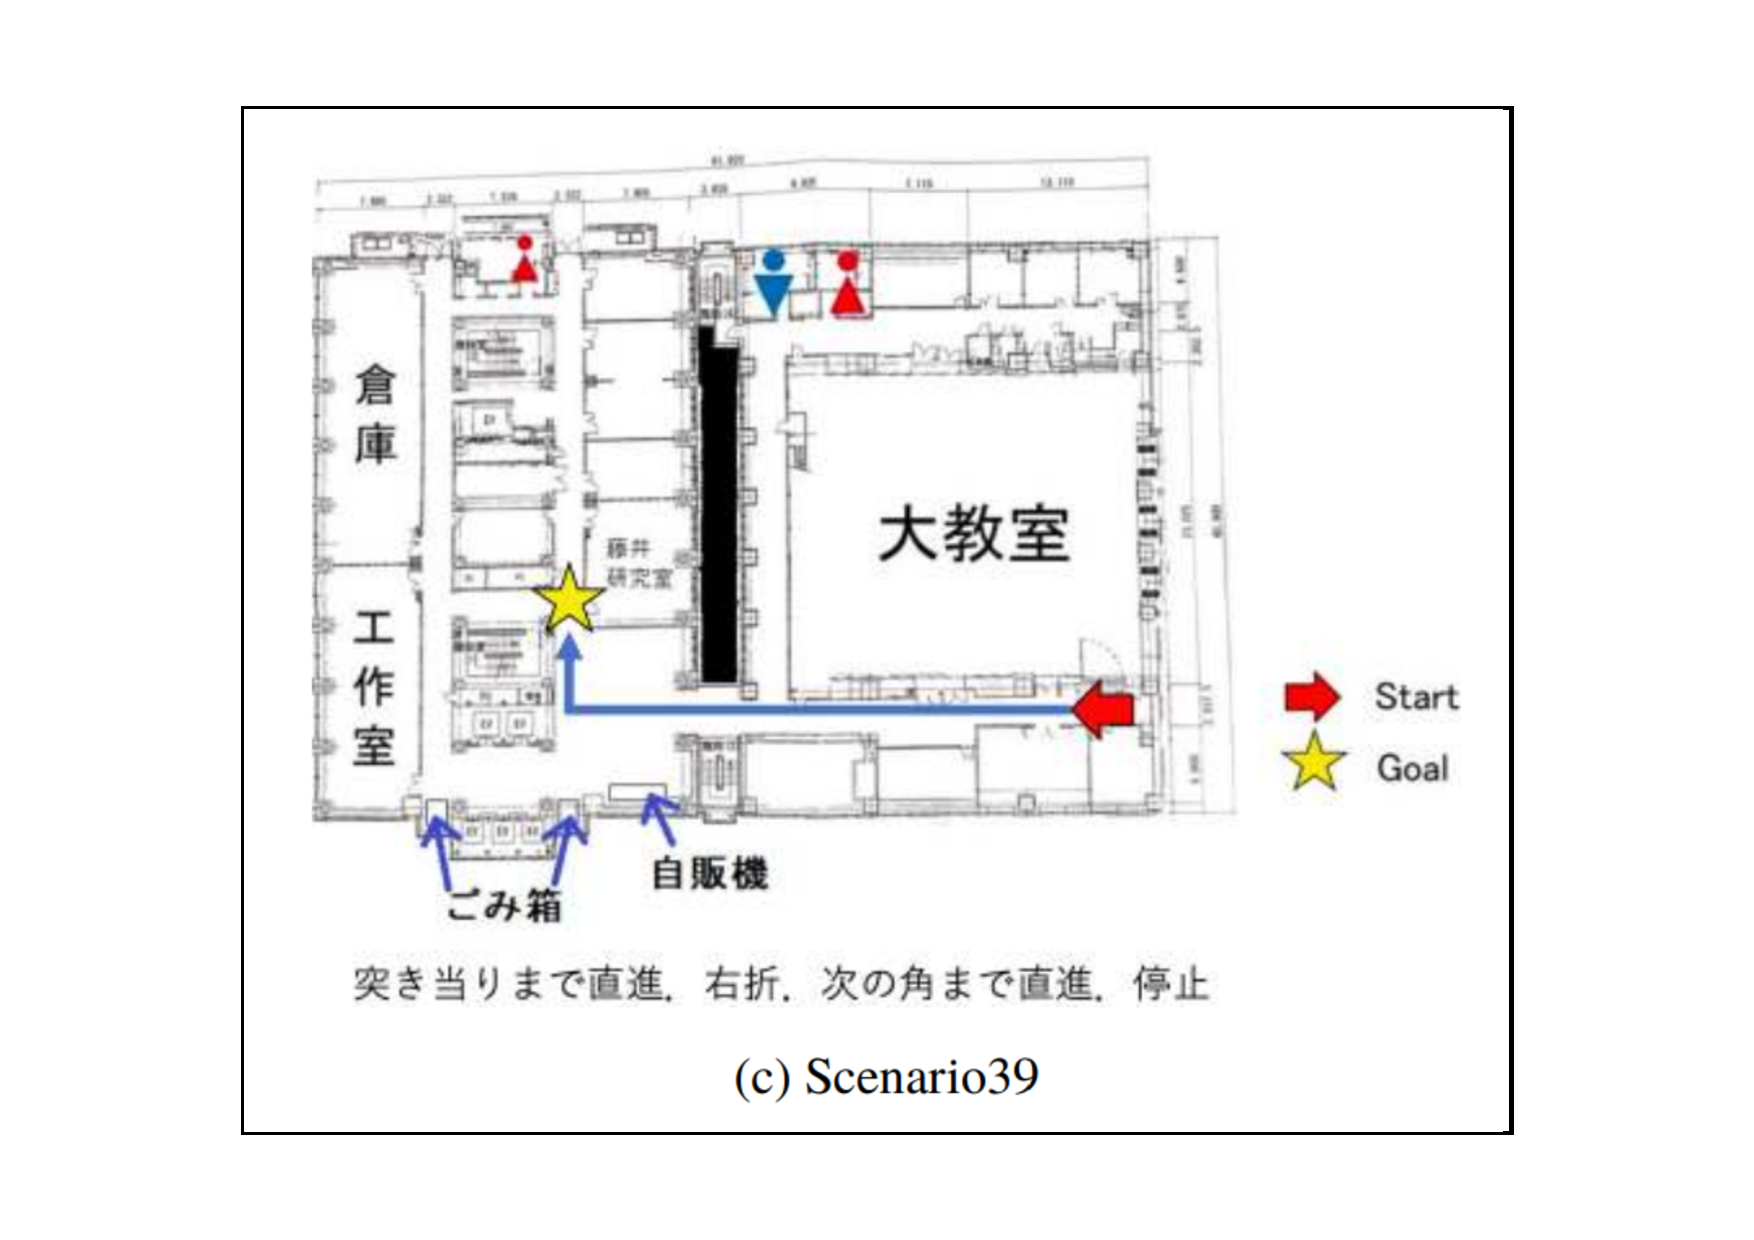
\includegraphics[keepaspectratio, width=80mm]{images/pdf/ishiguro/scenario/39.pdf}
        \subcaption{scenario39}
      \end{minipage}
  \end{tabular}
\caption{Scenarios 34 to 39}
\label{fig:scenario_34_39}
\end{figure*}

\begin{figure*}[htbp]
  \begin{tabular}{cc}
      \begin{minipage}[t]{0.48\textwidth}
        \centering
        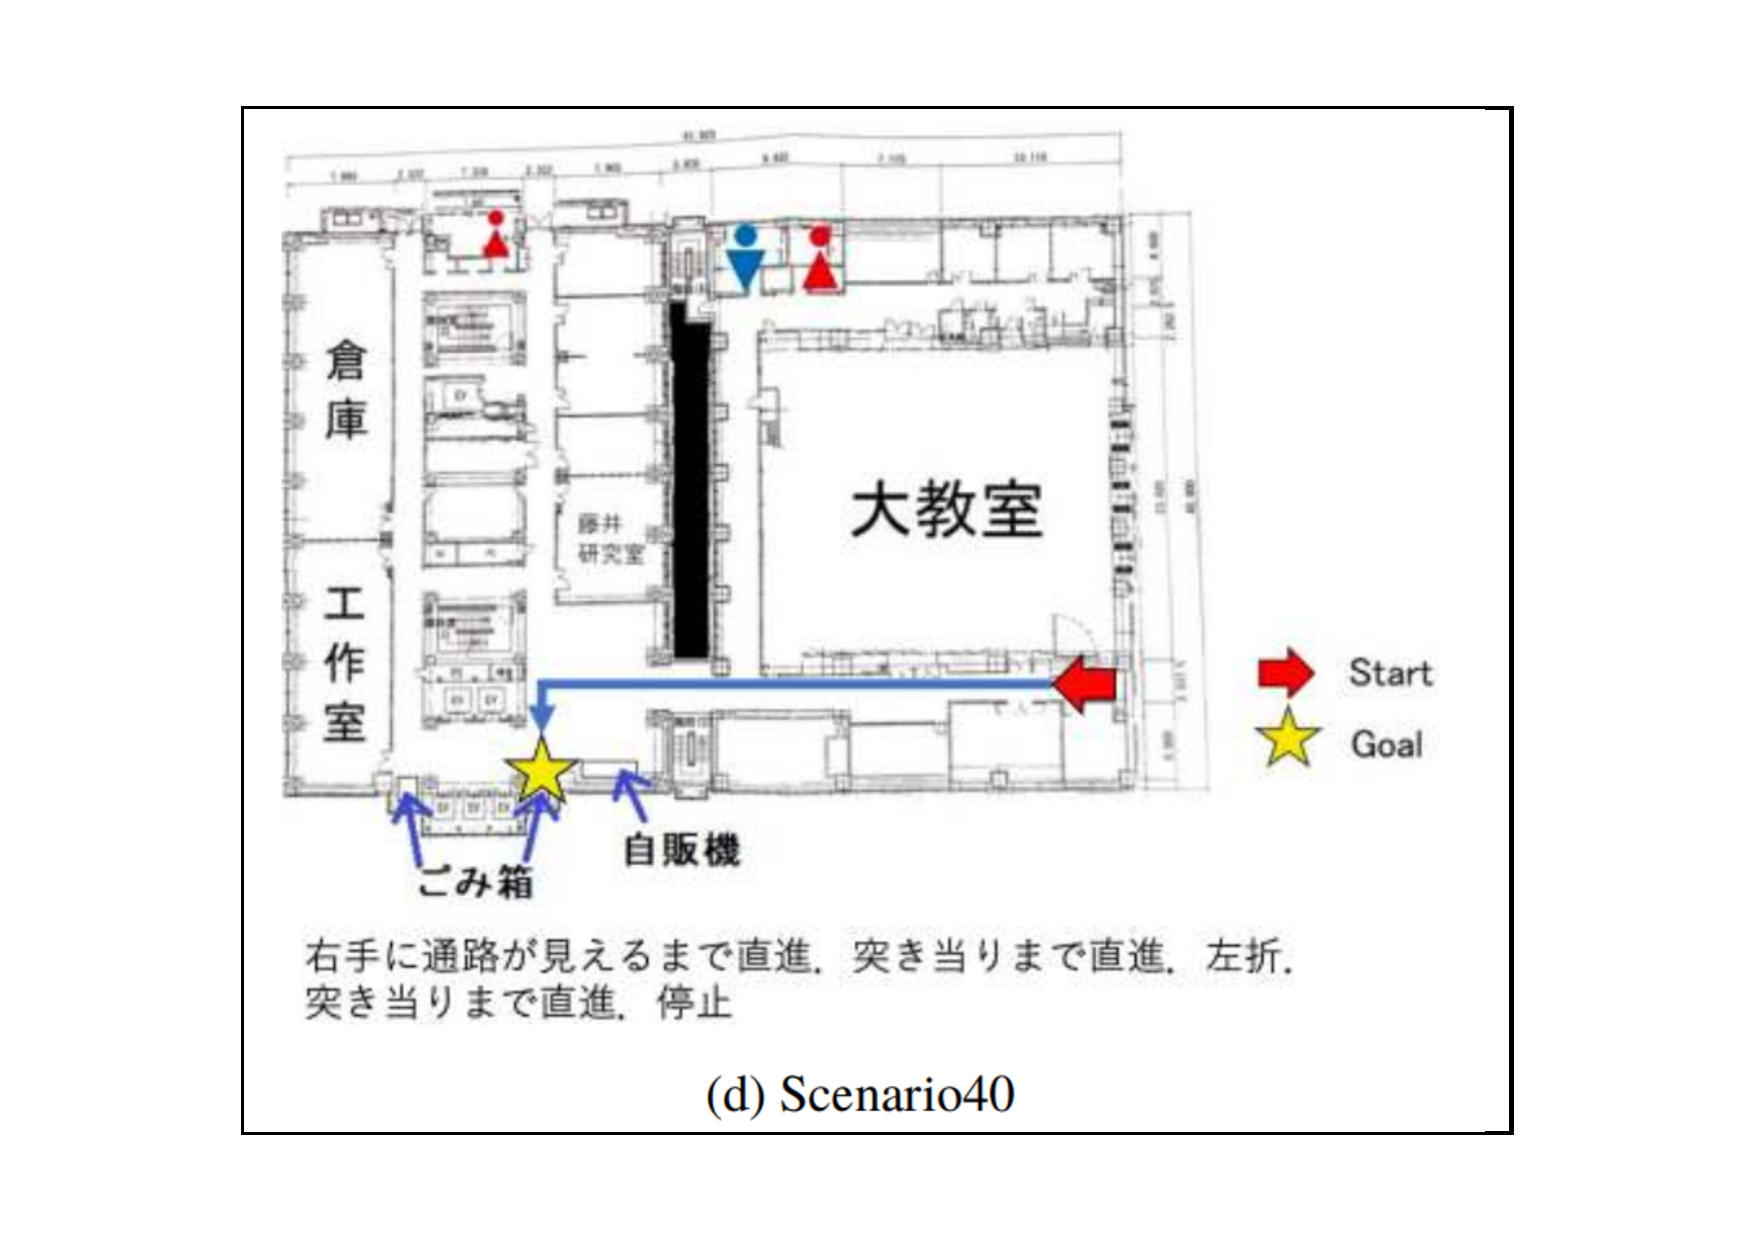
\includegraphics[keepaspectratio, width=80mm]{images/pdf/ishiguro/scenario/40.pdf}
        \subcaption{scenario40}
      \end{minipage} &
      \begin{minipage}[t]{0.48\textwidth}
        \centering
        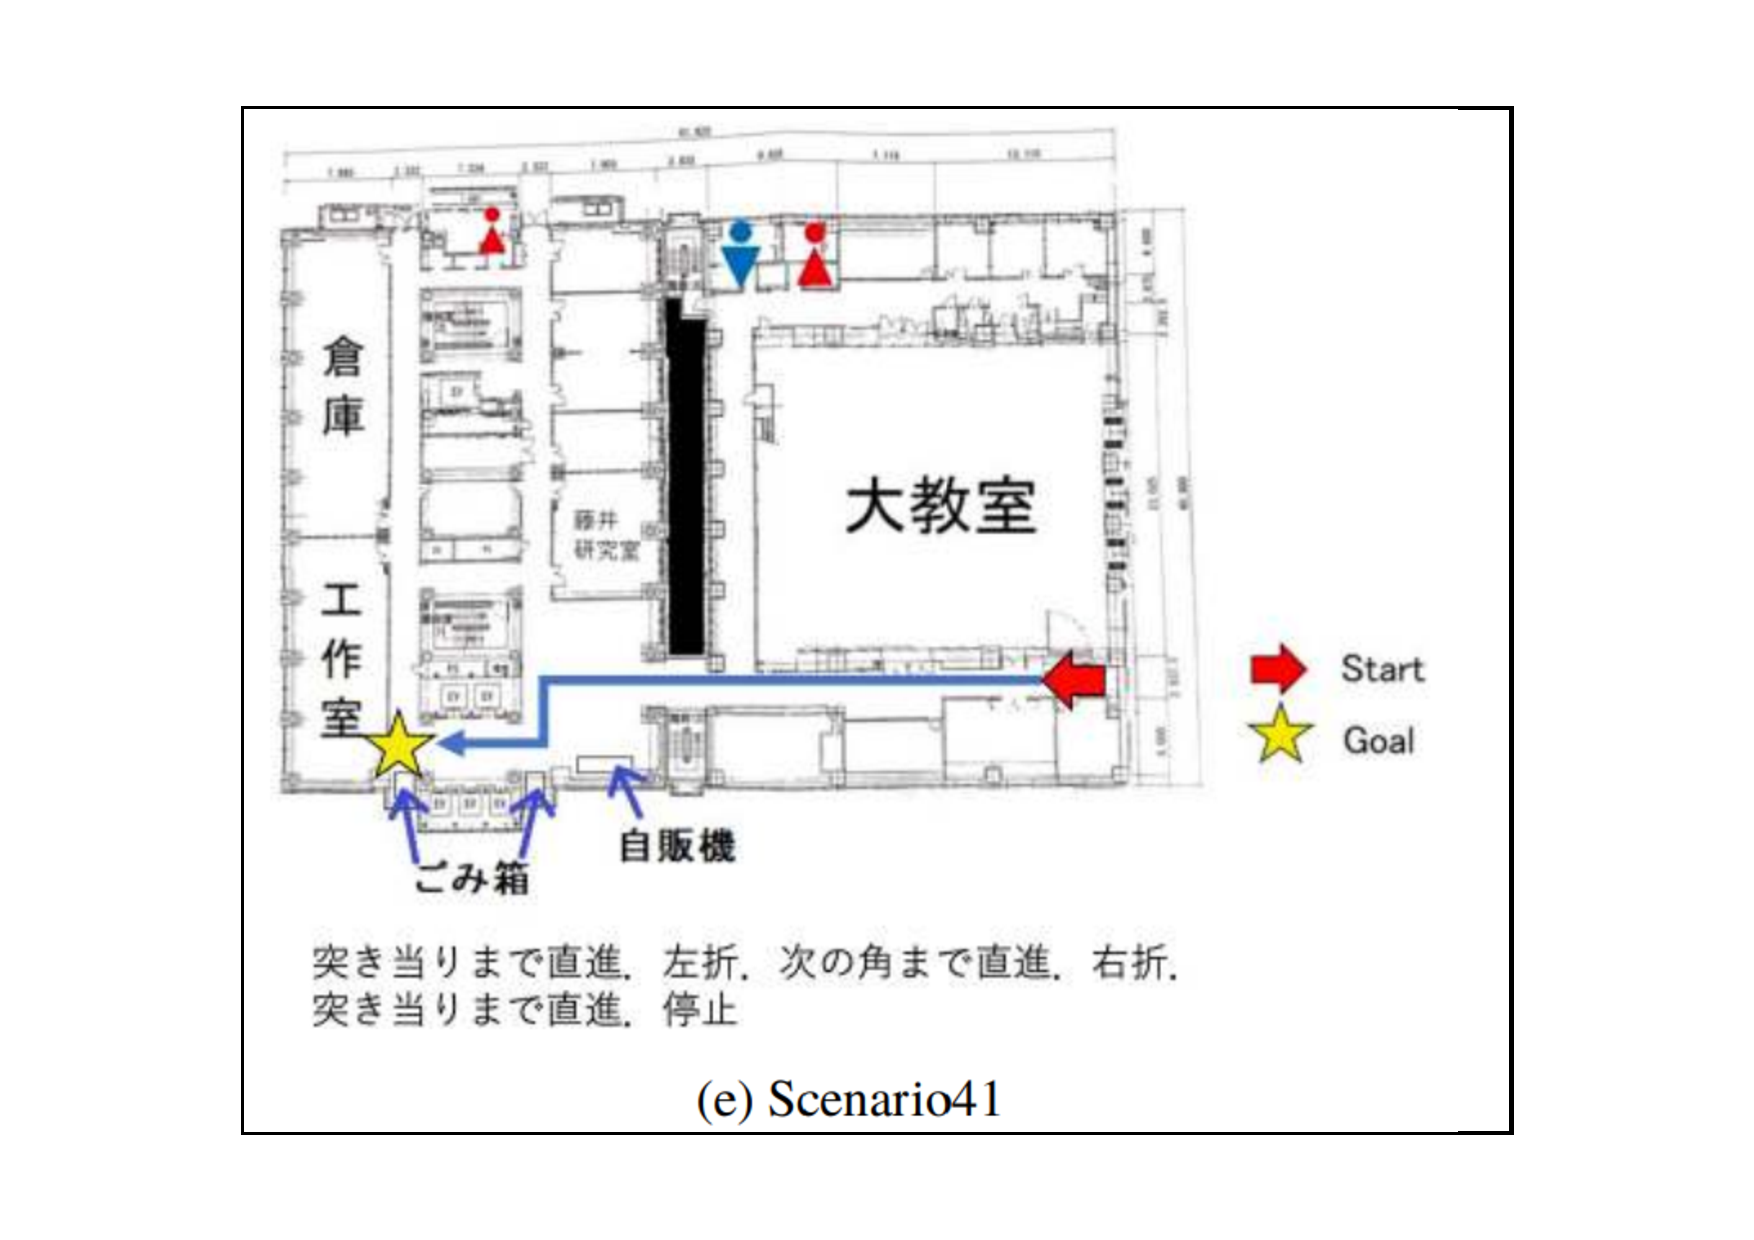
\includegraphics[keepaspectratio, width=80mm]{images/pdf/ishiguro/scenario/41.pdf}
        \subcaption{scenario41}
      \end{minipage} \\
      \begin{minipage}[t]{0.48\textwidth}
        \centering
        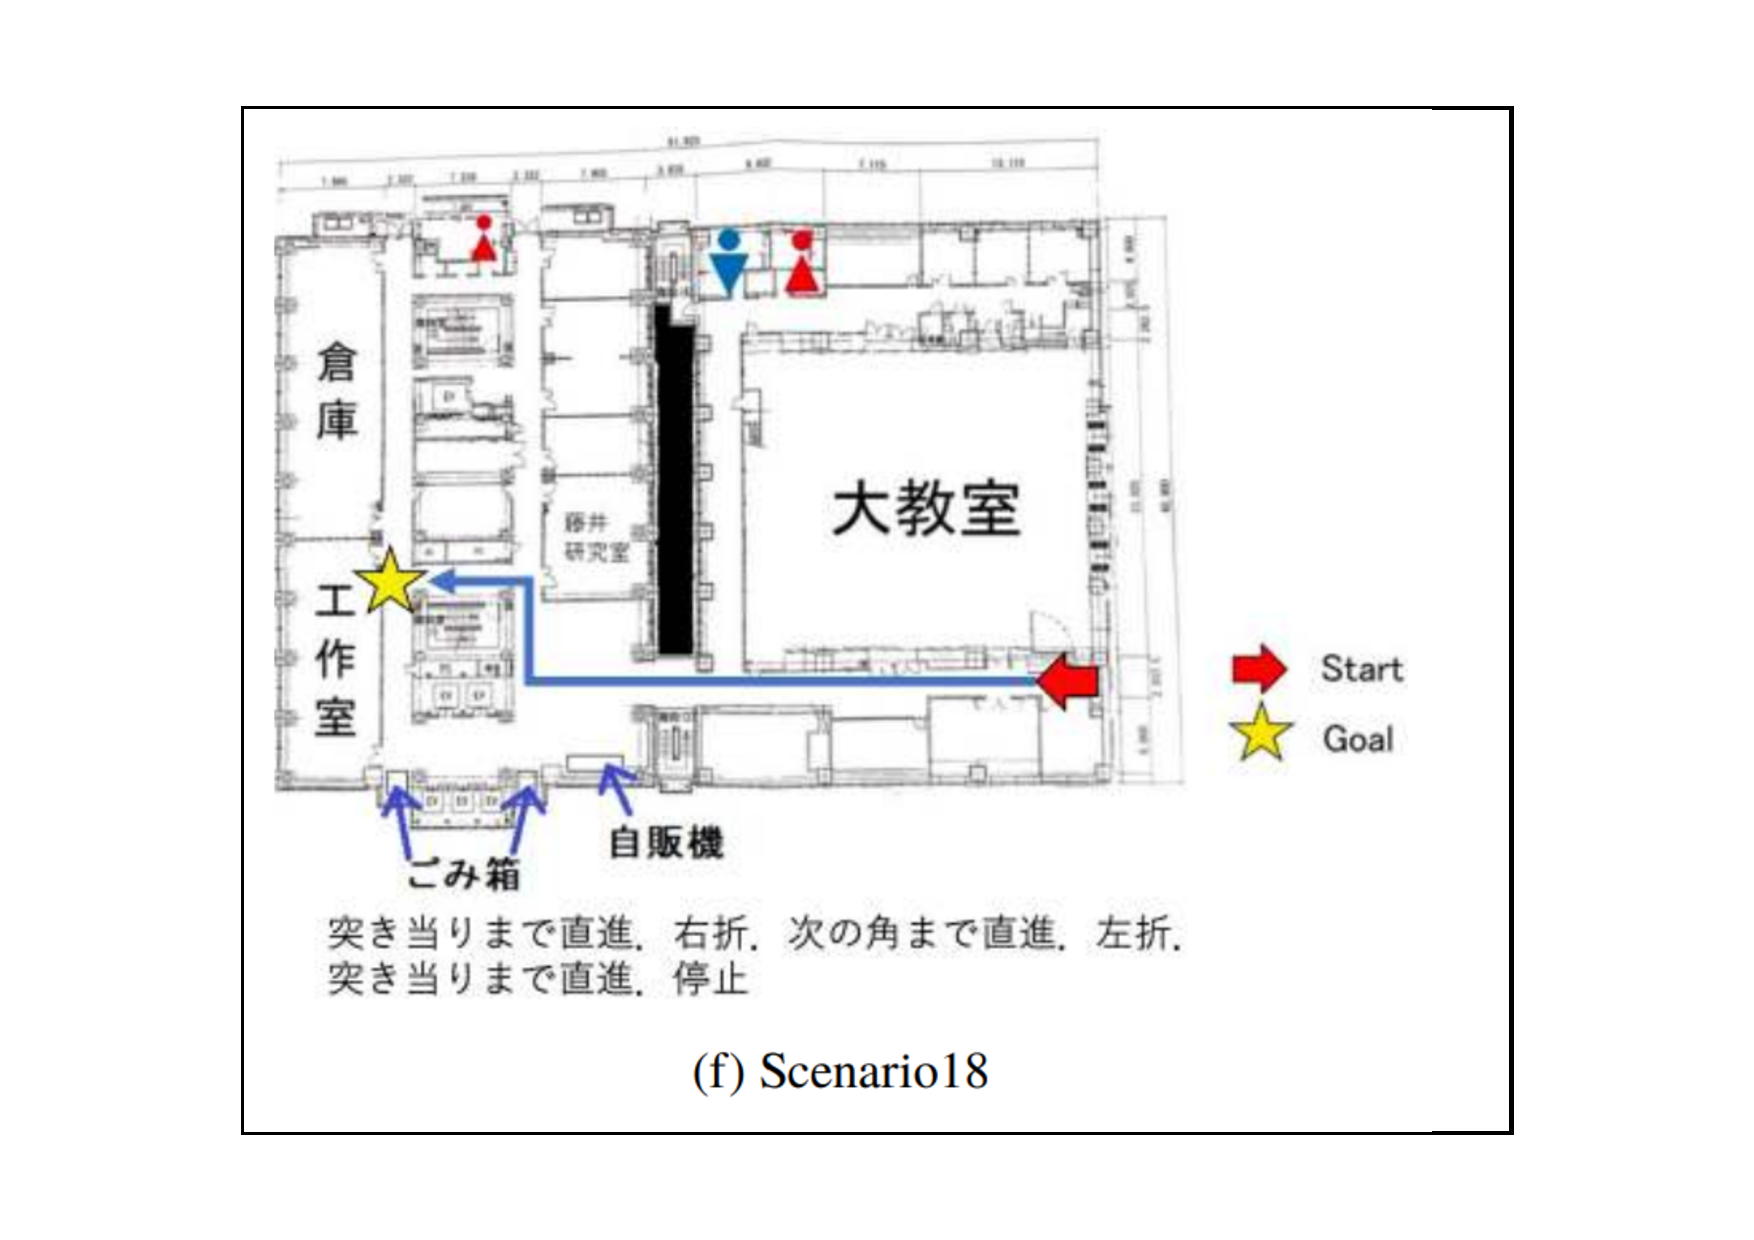
\includegraphics[keepaspectratio, width=80mm]{images/pdf/ishiguro/scenario/42.pdf}
        \subcaption{scenario42}
      \end{minipage} &
      \begin{minipage}[t]{0.48\textwidth}
        \centering
        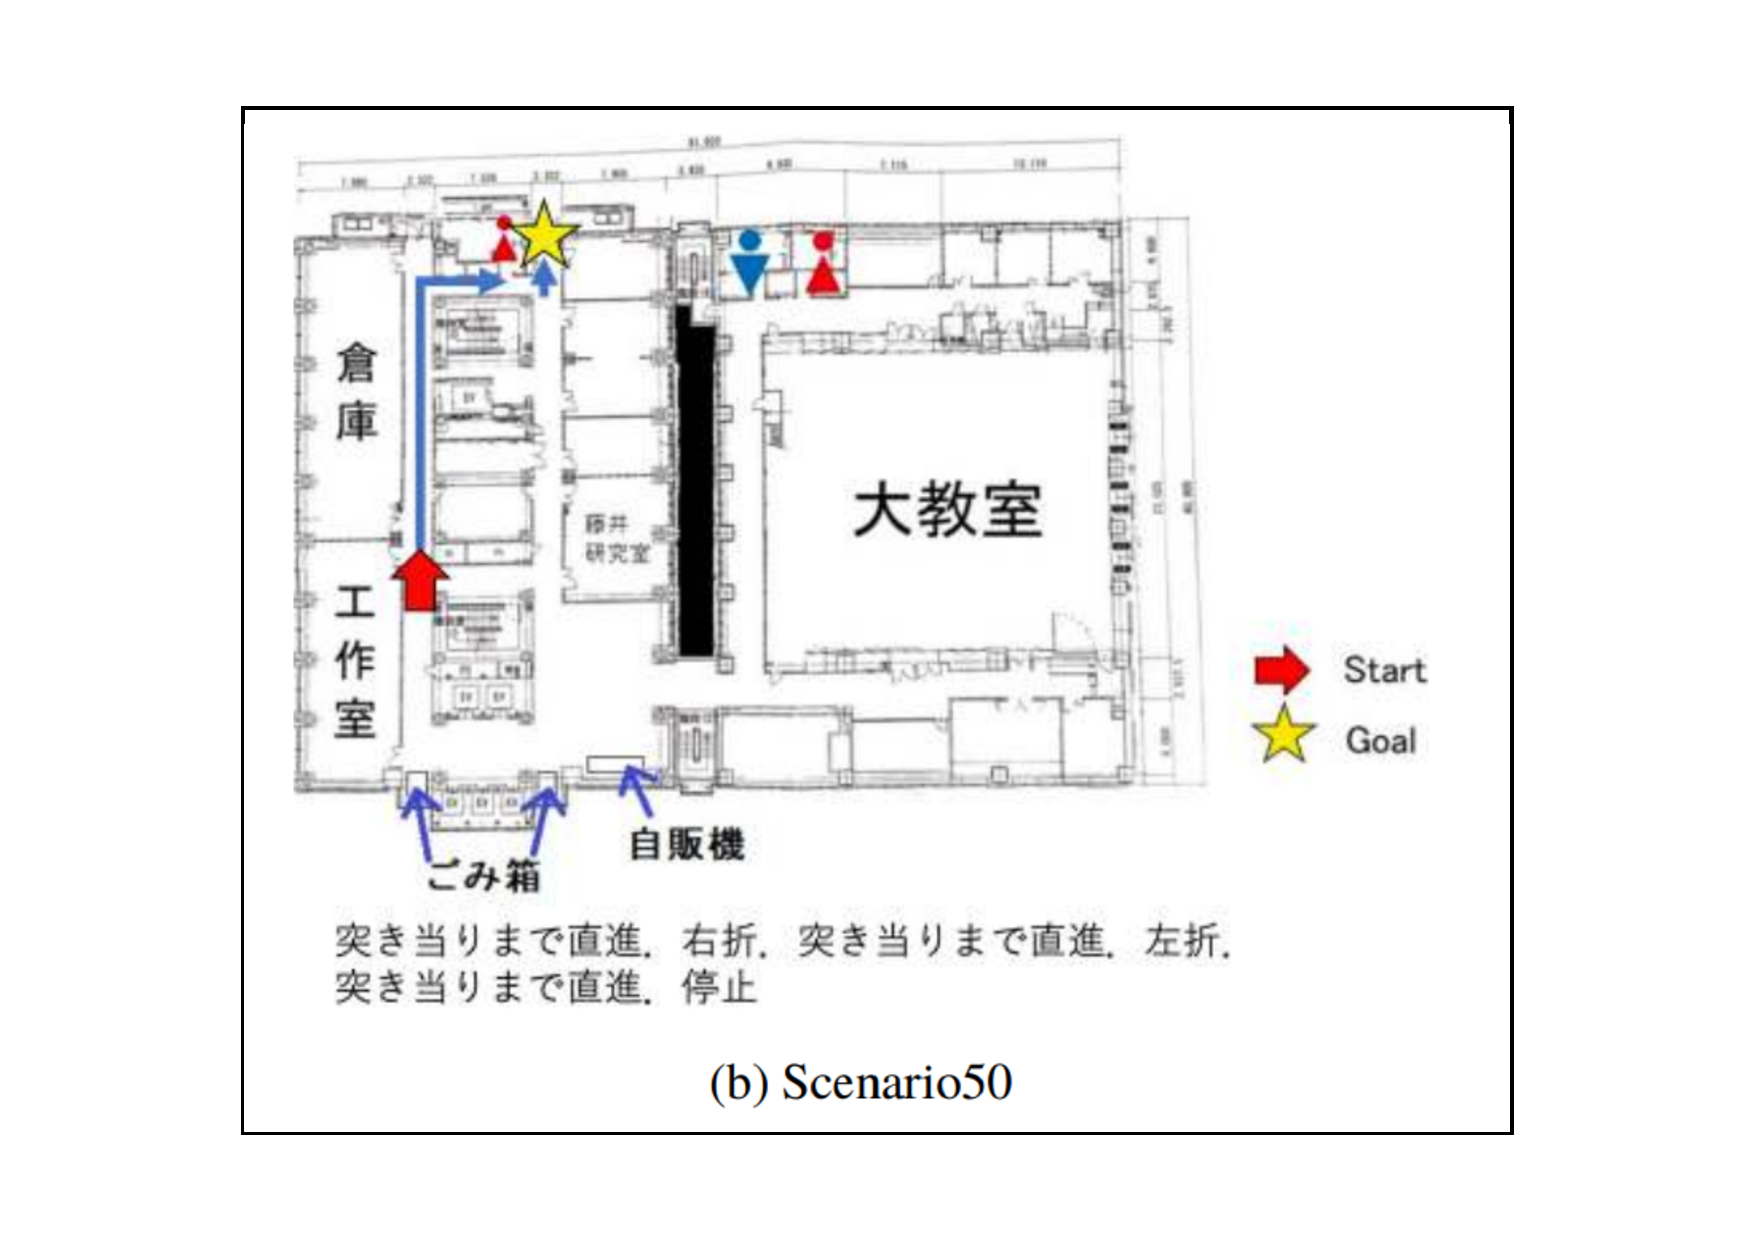
\includegraphics[keepaspectratio, width=80mm]{images/pdf/ishiguro/scenario/50.pdf}
        \subcaption{scenario50}
      \end{minipage}
  \end{tabular}
\caption{Scenarios 40 to 50}
\label{fig:scenario_40_50}
\end{figure*}

%
%!TEX root = ../thesis.tex
\chapter*{謝辞}
\addcontentsline{toc}{chapter}{謝辞}

本研究を進めるにあたり,幾度も研究相談や貴重なアドバイスをくださった林原靖男教授に,心より感謝申し上げます.
研究者として未熟な私でしたが,丁寧にご指導いただいたおかげで卒業論文という形にまとめることができました.

また,実験を手伝っていただいた佐藤君,塩田君,石原君には,多大なご協力をいただきました.
特に,夜遅くまで実験に付き合ってくださったことには感謝の念に堪えません.
本当にありがとうございました.

最後に,大学生活全般を支え,常に励ましてくれた両親に深く感謝します.
%


%

\end{document}
